\documentclass[journal,12pt,onecolumn,draftclsnofoot]{IEEEtran}

% --- CORE PACKAGES ---
\usepackage{cite}
\usepackage{amsmath,amssymb,amsfonts}
\usepackage{algorithmic}
\usepackage{algorithm}
\usepackage{graphicx}
\usepackage{textcomp}
\usepackage{xcolor}
\usepackage{geometry}
\usepackage{booktabs}
\usepackage{multirow}
\usepackage{bm}
\usepackage{longtable} 
\usepackage{fancyhdr}
\usepackage{lastpage}
\usepackage{subcaption}
\usepackage{hyperref}

% --- HYPERREF CONFIGURATION ---
\hypersetup{
    colorlinks=true,
    linkcolor=black,
    urlcolor=blue,
    citecolor=green,
    linktoc=all,
}

% --- PAGE GEOMETRY & SPACING ---
\linespread{1.5}
\geometry{a4paper, margin=1in}

% --- FOOTER CONFIGURATION ---
\pagestyle{fancy}
\fancyhf{} 
\renewcommand{\headrulewidth}{0pt} 
\fancyfoot[C]{\thepage\ of \pageref{LastPage}} 

\fancypagestyle{plain}{
    \fancyhf{}
    \renewcommand{\headrulewidth}{0pt}
    \fancyfoot[C]{\thepage\ of \pageref{LastPage}}
}

% --- SCIENTIFIC CHAPTER & NUMBERING SYSTEM ---
\makeatletter

% 1. Define chapter counter
\newcounter{chapter}

% 2. Numbering formats
\renewcommand{\thechapter}{\arabic{chapter}}
\renewcommand{\thesection}{\thechapter.\arabic{section}}
\renewcommand{\thesubsection}{\thesection.\arabic{subsection}}
\renewcommand{\thesubsubsection}{\thesubsection.\arabic{subsubsection}}

% 3. Link Counters to Chapters
\@addtoreset{section}{chapter}
\@addtoreset{figure}{chapter}
\@addtoreset{table}{chapter}
\@addtoreset{equation}{chapter}

\renewcommand{\thefigure}{\thechapter.\arabic{figure}}
\renewcommand{\thetable}{\thechapter.\arabic{table}}
\renewcommand{\theequation}{\thechapter.\arabic{equation}}

% 4. IEEEtran Indentation Display
\newcommand{\thechapterdis}{\thechapter.\quad} 
\renewcommand{\thesectiondis}{\thesection.\quad}
\renewcommand{\thesubsectiondis}{\thesubsection.\quad}
\renewcommand{\thesubsubsectiondis}{\thesubsubsection.\quad}

% 5. THE FIX: The Chapter command MUST alert the List of Figures
\newcommand{\my@chapter}[1]{%
    \cleardoublepage 
    \par\vspace*{4ex}%
    \refstepcounter{chapter}%
    % Force reset for safety
    \setcounter{section}{0}%
    \setcounter{figure}{0}%
    \setcounter{table}{0}%
    \setcounter{equation}{0}%
    % Add entry to Table of Contents
    \addcontentsline{toc}{chapter}{\protect\numberline{\thechapter}#1}%
    % THE CRITICAL MISSING LINK: Tell LOF and LOT to add space for the new chapter
    \addtocontents{lof}{\protect\addvspace{10\p@}}%
    \addtocontents{lot}{\protect\addvspace{10\p@}}%
    {\noindent\normalfont\Huge\bfseries Chapter \thechapter \par\vspace{2ex}\noindent\huge #1\par}%
    \@afterheading
    \vspace*{4ex}%
}

\newcommand{\my@schapter}[1]{% For \chapter*{...}
    \cleardoublepage
    \par\vspace*{4ex}%
    {\noindent\normalfont\Huge\bfseries #1\par}%
    \@afterheading
    \vspace*{4ex}%
}

\def\chapter{\@ifstar{\my@schapter}{\my@chapter}}

% 6. Section Styling
\renewcommand{\section}{\@startsection{section}{1}{\z@}%
    {3.5ex \@plus 1ex \@minus .2ex}%
    {2.3ex \@plus.2ex}%
    {\normalfont\Large\bfseries}}

\renewcommand{\subsection}{\@startsection{subsection}{2}{\z@}%
    {3ex \@plus 1ex \@minus .2ex}%
    {1.5ex \@plus.2ex}%
    {\normalfont\large\bfseries}}

% 7. TOC Formatting for Chapters
\newcommand*\l@chapter[2]{%
    \ifnum \c@tocdepth >\m@ne
    \addpenalty{-\@highpenalty}%
    \vskip 1.0em \@plus\p@
    \setlength\@tempdima{2.5em}% Increased for "Chapter X" width
    \begingroup
    \parindent \z@ \rightskip \@pnumwidth
    \parfillskip -\@pnumwidth
    \leavevmode \bfseries
    \advance\leftskip\@tempdima
    \hskip -\leftskip
    #1\nobreak\hfil \nobreak\hb@xt@\@pnumwidth{\hss #2}\par
    \penalty\@highpenalty
    \endgroup
    \fi}

\makeatother

\begin{document}

\begin{figure}[htbp]
    \centering
    \begin{subfigure}[t]{0.45\textwidth}
        \flushleft
        \IfFileExists{Alexandria_university.png}{%
            
\includegraphics[height=3cm]{Alexandria_university.png}%
        }{%
            \framebox[3cm]{\rule{0pt}{3cm} AU Logo}%
        }
    \end{subfigure}
    \hfill
    \begin{subfigure}[t]{0.45\textwidth}
        \flushright
        \IfFileExists{faculty_of_engineering.jpeg}{%
            
\includegraphics[height=3cm]{faculty_of_engineering.jpeg}%
        }{%
            \framebox[3cm]{\rule{0pt}{3cm} Faculty Logo}%
        }
    \end{subfigure}
    
    \vspace{0.5cm}
    \hrule height 0.4pt width \textwidth
\end{figure}

\begin{center}
Faculty of Engineering\\
    Department of Computer and Systems Engineering
\end{center}

\vspace{1cm} % Add some breathing room before the title

\begin{center}
    {\Large \textbf{Reference-Guided Few-Shot Segmentation with Foundation Models}} \\ 
    \vspace{0.5cm}
    {\large \textbf{PhD Research Proposal}}
\end{center}

\begin{center}
    In\\
    \vspace{0.5cm}
    {\large \textbf{Computer and Systems Engineering}}\\
\end{center}

\vspace{0.1cm}


\begin{center}
    Presented by\\
    \vspace{0.5cm}
    {\large \textbf{Omar Ahmed Fouad Hassan Wasfy}}\\
\end{center}

\vspace{0.1cm}

\begin{center}
    {\small \textbf{B.Sc. in Computer and Systems Engineering  \\
    Faculty of Engineering, Alexandria University, 2019}}
    
    \vspace{0.5cm}
    
    {\small \textbf{M.Sc. in Computer and Systems Engineering  \\
    Faculty of Engineering, Alexandria University, 2024}}
\end{center}

\vspace{1cm}

\begin{center}
    \textbf{Supervisors: Prof. Dr. Mohamed Ismail and Prof. Dr. Nagia Ghanem}
\end{center}

\vfill % Pushes the date to the bottom of the page

\begin{center}
   \textbf{2026}
\end{center}

\normalsize

\newpage

\begin{abstract}
Reference-guided few-shot segmentation with foundation models addresses open-set, class-agnostic dense prediction by leveraging a limited set of annotated support examples to segment unseen objects in query images. While vision foundation models such as the Segment Anything Model (SAM) provide strong geometric priors, they lack intrinsic mechanisms for semantic alignment across images, resulting in a semantic--geometric gap that limits their direct applicability to few-shot scenarios.  

This report presents a structured review of recent approaches that attempt to bridge this gap. A taxonomy is introduced to organize existing methods into prompt-based adaptation, probabilistic prompting, feature matching, consistency-based learning, graph-based reasoning, prototype-based modeling, personalized adaptation, and domain-specific adaptation. The report summarizes their core ideas, architectural components, and trade-offs, and discusses their behavior across commonly used benchmarks, including PASCAL-5i, COCO-20i, LVIS, and part-level datasets.  

In addition, the report documents the work completed so far during the PhD, including reproduction of selected methods and experimental results obtained from these implementations. These experiments provide practical insights into the behavior of different approaches, particularly with respect to prompt sensitivity, robustness in complex scenes, and handling of structural variations.  

Based on this analysis, the report identifies a set of research directions to be explored in the next phases of the PhD, focusing on improving robustness and generalization through more effective conditioning mechanisms and better handling of domain variability. The report therefore serves as both a consolidation of existing work and a foundation for the planned research.
\end{abstract}

\newpage
\tableofcontents
\newpage

% --- List of Figures ---
\cleardoublepage 
\phantomsection 
\addcontentsline{toc}{chapter}{List of Figures}
\listoffigures
\vspace{2em}

% --- List of Tables ---
\cleardoublepage
\phantomsection
\addcontentsline{toc}{chapter}{List of Tables}
\listoftables
\vspace{2em}

% --- List of Abbreviations ---
\cleardoublepage
\phantomsection
\addcontentsline{toc}{chapter}{List of Abbreviations}
\chapter*{List of Abbreviations}
\begin{IEEEdescription}[\IEEEsetlabelwidth{PASCAL-Part}]
    \item[BCE] Binary Cross-Entropy
    \item[CNN] Convolutional Neural Network
    \item[COCO-20i] Common Objects in Context (Few-Shot Split)
    \item[CV] Computer Vision
    \item[DAVIS] Densely Annotated VIdeo Segmentation
    \item[DOC] Cup Overlap Dice
    \item[DOD] Disc Overlap Dice
    \item[DSC] Dice Similarity Coefficient (Dice Score)
    \item[ELBO] Evidence Lower Bound
    \item[EMD] Earth Mover's Distance
    \item[FCN] Fully Convolutional Network
    \item[FPS] Frames Per Second
    \item[FSS] Few-Shot Segmentation
    \item[GFLOPs] Giga Floating Point Operations
    \item[KL] Kullback-Leibler (Divergence)
    \item[LVIS] Large Vocabulary Instance Segmentation
    \item[MAE] Masked Autoencoder
    \item[mIoU] Mean Intersection over Union
    \item[NLP] Natural Language Processing
    \item[PACO] Parts and Attributes of Common Objects
    \item[PASCAL-5i] PASCAL Visual Object Classes (Few-Shot Split)
    \item[PEFT] Parameter-Efficient Fine-Tuning
    \item[PMC] Point-Mask Clustering
    \item[PNA] Positive-Negative Alignment
    \item[SAM] Segment Anything Model
    \item[ViT] Vision Transformer
    \item[VRP] Visual Reference Prompt
\end{IEEEdescription}
\newpage

% ==========================================
% CHAPTER 1: INTRODUCTION AND PROBLEM FORMULATION
% ==========================================
\chapter{Introduction and Problem Formulation}

\section{Background and Motivation}
Semantic segmentation, the computational process of assigning a categorical class label to every individual pixel within an image, is a cornerstone of modern computer vision. Traditionally, achieving state-of-the-art performance in this domain relies on supervised learning paradigms that require massive, densely annotated datasets. Architectures such as Fully Convolutional Networks (FCNs) and the DeepLab series optimize millions of parameters to recognize a fixed, predefined set of categories. 

However, this closed-set paradigm exhibits catastrophic performance degradation when tasked with segmenting objects outside its original training distribution. The rigidity of standard semantic segmentation lacks the flexibility required for dynamic, real-world applications such as medical imaging analysis, autonomous navigation, and industrial robotics where novel object categories emerge continuously. Furthermore, the acquisition of exhaustive pixel-level annotations for every new category is prohibitively expensive, time-consuming, and prone to human error.

Few-shot segmentation (FSS) directly addresses this fundamental limitation. By drawing inspiration from human cognitive capabilities, FSS aims to adapt neural networks to unseen, novel classes using only a minimal support set (reference set) of annotated examples typically ranging from 1 to 5 images. The recent integration of vision foundation models, trained on unprecedented scales of unannotated or semi-annotated data, introduces powerful zero-shot generalization capabilities. Adapting these foundation models for few-shot tasks represents a massive paradigm shift in computer vision: moving away from training specialized architectures from scratch, toward engineering efficient, lightweight mechanisms to condition frozen, billion-parameter networks.

\section{Problem Statement}
Reference-guided few-shot segmentation specifically aims to produce an accurate pixel-level delineation of a target object in a query image given only a small support set (reference set) of annotated reference images. The core problem is structural and mathematical: how to map the semantic intent of the reference annotations into a latent format mathematically compatible with the foundation model's input prompt space. The primary objective is achieving precise semantic alignment across images characterized by severe appearance variability, without inducing catastrophic forgetting of the foundation model's heavily optimized, pre-trained geometric priors.



\section{Research Scope and Objectives}
This doctoral proposal report systematically evaluates the methodological progression of conditioning mechanisms for the Segment Anything Model (SAM) in few-shot scenarios, documents the foundational experimental work completed to date, and outlines the trajectory for future research. The primary objectives are to:
\begin{enumerate}
    \item Analyze state-of-the-art adaptation techniques, tracing the evolution from basic prompt engineering and feature aggregation to complex probabilistic spaces, prototype matching, and topological graph-based architectures.
    \item Dissect the mathematical formulations and architectural implementations of these models, specifically evaluating their feature extraction pipelines, cross-attention mechanisms, and custom loss functions.
    \item Compare empirical performance across standard FSS benchmarks (COCO-20i, PASCAL-5i), large-vocabulary benchmarks (FSS-1000, LVIS-92i), personalized datasets (PerSeg, DAVIS 2017), and medical domain tasks.
    \item Define the theoretical and practical limits of current approaches regarding computational complexity, inference latency, memory footprint, and multi-shot scaling capabilities.
    \item Replicate and empirically validate selected state-of-the-art architectures (e.g., VRP-SAM, Bridge-the-Points, PerSAM, DAPSAM) to establish highly reliable performance baselines.
    \item Formulate and test targeted architectural enhancements---such as weight-averaging model soups, temporal memory banks, and domain-adaptive residual scaling---to systematically mitigate identified failure modes.
    \item Propose novel research directions and a phased execution plan for the remainder of the doctoral studies, specifically targeting the multi-shot degradation problem and cross-domain robustness.
\end{enumerate}

\section{Contributions of the Study}
The primary contributions of this synthesis and the completed experimental work are:
\begin{itemize}
    \item The establishment of a formalized methodological taxonomy for SAM adaptation techniques, categorizing the current literature based on their foundational approach to the semantic-geometric gap.
    \item A detailed algorithmic deconstruction of foundational methodologies, highlighting their mathematical novelties, specifically regarding positive-negative alignment, variational inference, and domain adaptation.
    \item A critical synthesis of empirical results across distinct datasets, explicitly correlating mIoU performance with dataset complexity in 1-shot and 5-shot configurations.
    \item The identification of systemic failure modes related to scale variation, prompt sensitivity, and dense multi-instance clutter.
    \item The successful reproduction of diverse SAM-adaptation frameworks, establishing verified empirical baselines across standard, personalized, and clinical domains.
    \item The implementation and validation of targeted methodological enhancements---including Iterative Uniform Greedy Model Soups for VRP-SAM, temporal memory banks for zero-shot video segmentation, and optimized residual scaling for medical adaptation---yielding measurable quantitative improvements.
    \item The articulation of a comprehensive, phased PhD research plan designed to systematically resolve the identified multi-shot degradation and cross-domain scalability bottlenecks.
\end{itemize}


\section{Task Definition and Episodic Paradigm}
Reference-guided few-shot segmentation with foundation models is a conditional dense prediction task. It aims to produce an accurate pixel-level delineation of a target object in a query image (target image) using only a small set of annotated reference examples. Each reference example consists of an image paired with a segmentation mask specifying the object of interest. This reference set functions as an explicit task descriptor at inference time, enabling the model to segment the same object in previously unseen images without retraining or relying on predefined category labels.

Unlike conventional semantic segmentation, which assumes a fixed set of classes learned during training, this paradigm operates in an open-set and class-agnostic setting. The system must generalize to novel object categories and domains based solely on the visual information contained in the reference examples. This flexibility is essential for real-world scenarios where exhaustive annotation of all possible object categories is infeasible.

The task operates under the standard $N$-way $K$-shot episodic formulation. The support set (reference set)  $S = \{(I_{s,i}, M_{s,i})\}_{i=1}^K$ consists of $K$ reference images and their corresponding ground-truth binary masks for a specific target class $c$. The episodic training paradigm mimics the inference environment, assuming access to a massive training dataset $\mathcal{D}_{train}$ containing base classes $\mathcal{C}_{base}$. The model is subsequently evaluated on a disjoint testing dataset $\mathcal{D}_{test}$ containing strictly novel classes $\mathcal{C}_{novel}$, ensuring that $\mathcal{C}_{base} \cap \mathcal{C}_{novel} = \emptyset$.

\section{Mathematical Input and Output Representation}
The system receives two complementary components that define the task. First, the \textbf{Support Set (Reference Set)} provides the semantic and visual definition of the target. These high-resolution RGB images are normalized and resized to accommodate the foundation model's Vision Transformer backbone:
\begin{equation}
    I_s, I_q \in \mathbb{R}^{H \times W \times 3}
\end{equation}
The binary support masks denote the precise spatial location of the foreground target object:
\begin{equation}
    M_s \in \{0, 1\}^{H \times W}
\end{equation}
This support set (reference set) acts as an explicit spatial attention mechanism. It typically contains one to five examples, representing an object instance or a semantic concept, and can exhibit variability in viewpoint, scale, appearance, and background.

Second, the \textbf{Query Image (Target Image)} ($I_q$) is an unlabeled image where the model must identify the object defined by the support set (reference set). Query images (Target images) may contain multiple objects, complex scenes, and conditions differing from the references.

The final output is a predicted dense probability map:
\begin{equation}
    \hat{M}_q \in [0, 1]^{H \times W}
\end{equation}
An effective prediction precisely delineates object boundaries, corresponds strictly to the reference object, excludes visually similar distractors, and remains robust to contextual variations. This probability map is subsequently thresholded (standardized at $\tau = 0.5$) to yield the discrete binary mask.

\section{Standard Loss Formulations}
Because the target objects in few-shot tasks often occupy a very small percentage of the total image area, models face severe class imbalance. During the meta-training of the auxiliary conditioning modules, models typically optimize a combination of Binary Cross-Entropy (BCE) Loss and Dice Loss:
\begin{equation}
    \mathcal{L}_{BCE} = -\frac{1}{N} \sum_{i=1}^N \left[ y_i \log(\hat{y}_i) + (1 - y_i) \log(1 - \hat{y}_i) \right]
\end{equation}
\begin{equation}
    \mathcal{L}_{Dice} = 1 - \frac{2 \sum_{i=1}^N y_i \hat{y}_i}{\sum_{i=1}^N y_i + \sum_{i=1}^N \hat{y}_i}
\end{equation}
The total loss is a weighted sum:
\begin{equation}
    \mathcal{L}_{total} = \mathcal{L}_{BCE}(\hat{M}_q, M_q) + \lambda \mathcal{L}_{Dice}(\hat{M}_q, M_q)
\end{equation}
where $\lambda$ is a balancing hyperparameter ensuring that small structural details are captured while maintaining overall pixel-wise accuracy.

\section{Core Technical Challenges}
Adapting generic foundation models to the strict parameters of FSS introduces several critical computational and mathematical bottlenecks:
\begin{itemize}
    \item \textbf{Cross-Image Correspondence:} Establishing reliable associations between reference and query regions despite differences in viewpoint, pose, illumination, and background context.
    \item \textbf{Appearance Variability:} Handling significant intra-class variation, scale changes, deformation, and partial occlusion between reference and target instances.
    \item \textbf{Distractor Suppression:} Distinguishing the target object from visually similar objects and densely cluttered environments.
    \item \textbf{Prompt Sensitivity:} Ensuring stable performance when reference annotations are sparse, imperfect, or when suboptimal prompts are generated by automated systems.
    \item \textbf{Adaptation Without Overfitting:} Specializing the foundation model to the reference object while maintaining its broad zero-shot geometric priors.
    \item \textbf{Computational Efficiency:} Achieving adaptation at inference time without expensive retraining.
\end{itemize}

\section{Applications}
Reference-guided few-shot segmentation enables adaptive perception in scenarios where labeled data is scarce or object categories are dynamic. Key applications include:
\begin{itemize}
    \item \textbf{Video Object Segmentation:} Segmenting a specific object across frames using a few annotated references.
    \item \textbf{Medical Image Analysis:} Segmenting rare anatomical structures or pathological regions using limited annotated cases.
    \item \textbf{Robotics and Autonomous Manipulation:} Allowing robots to recognize and interact with previously unseen objects specified through demonstrations.
    \item \textbf{Autonomous Driving and Intelligent Transportation:} Segmenting unexpected road hazards or rare obstacles using a few reference examples.
    \item \textbf{Image Editing and Content Creation:} Extracting objects specified by example images for compositing and generative workflows.
    \item \textbf{Visual Search and Retrieval:} Locating instances of a queried object within large image collections.
    \item \textbf{Surveillance and Multi-Object Tracking:} Monitoring specific targets across scenes without predefined class labels.
    \item \textbf{Industrial Inspection and Quality Control:} Detecting defects or anomalies using minimal annotated samples.
    \item \textbf{Remote Sensing and Earth Observation:} Segmenting environmental features from satellite imagery using few references.
    \item \textbf{Augmented and Mixed Reality:} Identifying user-specified objects in real time for interactive overlays.
\end{itemize}

\newpage

\section{Report Structure}
The remainder of this proposal is organized as follows:

\begin{itemize}
    \item \textbf{Chapter 2: Theoretical Background, Related Work, and Recent Advances:} Covers the evolution of semantic segmentation, the architecture of vision foundation models (specifically SAM), establishes the methodological taxonomy, and provides a critical analysis of recent advances in the field.
    \item \textbf{Chapter 3: Benchmarking, Evaluation Metrics, and Comparative Results:} Details the benchmark datasets, defines the quantitative evaluation metrics (e.g., mIoU, Dice Score), and presents a comprehensive comparative study of state-of-the-art performance across standard, large-vocabulary, and medical domains.
    \item \textbf{Chapter 4: Technical Discussion:} Analyzes the critical trade-offs between representation quality, robustness, and computational efficiency, serving as a technical assessment of the current state of the field.
    \item \textbf{Chapter 5: Research Gaps and Bottlenecks:} Pinpoints specific failures and limitations in the current literature, notably the multi-shot degradation problem and the persistent semantic-geometric gap.
    \item \textbf{Chapter 6: Work Completed in the PhD So Far:} Documents the experimental reproductions, baseline comparisons, and targeted architectural enhancements successfully implemented during the initial phase of the research.
    \item \textbf{Chapter 7: Proposed PhD Research Directions:} Outlines the specific methodological approaches and technical innovations proposed to directly address the structural gaps identified in Chapter 5.
    \item \textbf{Chapter 8: Expected Contributions and Research Plan:} Details the anticipated academic and scholarly impact of the proposed research and provides a phased timeline for its execution.
    \item \textbf{Chapter 9: Conclusion:} Presents a final synthesis of the study's foundational insights and concludes the proposal.
\end{itemize}


\newpage

% ==========================================
% CHAPTER 2: THEORETICAL BACKGROUND, RELATED WORK, AND RECENT ADVANCES
% ==========================================
\chapter{Theoretical Background, Related Work, and Recent Advances}

\section{Evolution of Semantic Segmentation}
Early approaches to semantic segmentation relied heavily on Fully Convolutional Networks (FCNs), which replaced the dense, fully connected layers of classification networks with convolutional layers to output spatial maps. The introduction of residual connections via ResNet allowed for much deeper architectures, mitigating the vanishing gradient problem and vastly improving spatial feature extraction capabilities. Subsequent architectures like DeepLabv3 integrated Atrous Spatial Pyramid Pooling (ASPP) to capture multi-scale context. However, these models were strictly bounded by the closed-set nature of their training data (e.g., PASCAL VOC, MS COCO). They lacked the structural capacity to generalize to novel, out-of-distribution classes without extensive retraining or fine-tuning, severely limiting their real-world scalability.

\section{Few-Shot Segmentation via Metric Learning}
To overcome the limitations of closed-set classifiers, early Few-Shot Segmentation (FSS) approaches utilized metric learning and episodic training paradigms, heavily inspired by Prototypical Networks originally designed for few-shot image classification. These models, such as PANet \cite{wang2019panet} and PFENet \cite{tian2020pfenet}, functioned by projecting both support (reference) and query (target) images into a shared, highly optimized latent space. They subsequently computed pixel-wise cosine similarities between the query features and a generated "class prototype" extracted from the support mask. 

While highly effective on standard, moderately complex benchmarks, these early metric-learning models exhibited several critical flaws:
\begin{enumerate}
    \item They often overfitted to the base classes seen during the episodic training domains.
    \item The episodic training itself, required to simulate few-shot scenarios during the training phase, was computationally expensive and memory-intensive.
    \item They struggled with strict open-set generalization when encountering radically novel classes or extreme domain shifts (e.g., medical or satellite imagery).
\end{enumerate}

\section{Vision Foundation Models and Self-Supervision}
The landscape of computer vision shifted dramatically with the introduction of foundation models. These models leverage self-supervised or contrastive learning (e.g., Masked Autoencoders) over millions, or even billions, of unannotated images to produce highly robust, generalized feature embeddings. 

The Vision Transformer (ViT) revolutionized this space by discarding convolutions entirely. By treating image patches as linear sequences, ViTs allow multi-head self-attention mechanisms to capture long-range global context across the entire image, a feat previously inaccessible to localized CNN receptive fields.

Further advancements like DINOv2 \cite{oquab2023dinov2} demonstrated that self-supervised learning on curated, large-scale datasets could produce features with dense, part-level semantic understanding without any manual bounding-box or mask annotations. These models serve as universal feature extractors, forming the foundational backbone of modern perception systems and rendering training-from-scratch obsolete for most downstream tasks.

\section{Prompt Learning and Visual Conditioning}
Prompt learning, initially popularized in Large Language Models (LLMs) like GPT within Natural Language Processing (NLP), has transitioned successfully to computer vision. Visual prompting involves appending learnable parameters (tokens) to the input image patches or intermediate feature maps. This technique allows for task-specific adaptation while keeping the massive backbone weights (often comprising hundreds of millions of parameters) strictly frozen. This approach preserves the foundation model's generalized representation capacity and crucially minimizes the risk of overfitting during the few-shot adaptation phase, where training data is extremely scarce.

\section{Architecture of SAM}
The Segment Anything Model (SAM) is arguably the most prominent vision foundation model developed to date. It is designed to perform class-agnostic segmentation and consists of three highly optimized, distinct core components:

1. \textbf{Image Encoder:} A Masked Autoencoder (MAE) pre-trained Vision Transformer (typically ViT-H, containing 632 million parameters) that processes high-resolution inputs ($1024 \times 1024$) into a compact, highly expressive feature grid ($64 \times 64 \times 256$). This encoder is computationally heavy and represents the primary latency bottleneck of the model; however, it only needs to run once per image.
\\
2. \textbf{Prompt Encoder:} A lightweight module that embeds spatial prompts (points, bounding boxes, dense masks) and textual prompts into the 256-dimensional latent space.
\\
3. \textbf{Mask Decoder:} A highly efficient, lightweight two-way transformer block that iteratively updates image embeddings and prompt embeddings via bidirectional cross-attention, ultimately outputting multi-scale mask predictions.

\begin{figure}[htbp]
\centering
\IfFileExists{SAM.png}{%
    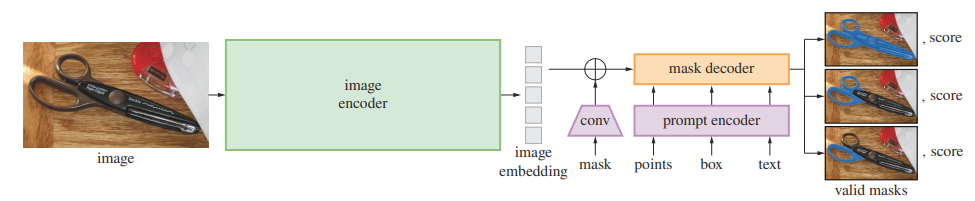
\includegraphics[width=1\linewidth]{SAM.png}%
}{%
    \framebox[\linewidth]{\rule{0pt}{200pt}\textbf{Missing Image: SAM.png}}%
}
\caption{Detailed architecture of the Segment Anything Model (SAM) highlighting the heavy Image Encoder, the flexible Prompt Encoder, and the lightweight, real-time Mask Decoder.}
\label{fig:SAM}
\end{figure}

\section{Prompting Mechanisms and Positional Encodings}
The prompt encoder handles different prompt types via distinct mathematical operations. It embeds discrete spatial prompts (points and bounding boxes) via continuous Fourier-based positional encodings, mapped to the exact coordinate space of the extracted image features:
\begin{equation}
    PE(x, y) = [\sin(2\pi \mathbf{B} [x,y]^T), \cos(2\pi \mathbf{B} [x,y]^T)]
\end{equation}
where $\mathbf{B}$ is a randomly initialized Gaussian matrix. 

Conversely, dense mask prompts are encoded using cascaded convolutional downsampling layers coupled with GELU activations. These encoded mask features are then summed element-wise directly with the ViT image embeddings prior to entering the two-way transformer decoder. 

\section{The Semantic-Geometric Gap}
SAM was trained using a highly rigorous data engine loop, resulting in the unprecedented SA-1B dataset containing over 11 million images and 1 billion high-quality masks. This training enforces extreme geometric robustness. While SAM exhibits unparalleled zero-shot generalization to unseen images and complex multi-object compositions, this generalization is strictly \textit{spatial and geometric}. 

The model identifies pristine boundaries and generates exceptional object proposals, but it \textit{does not} assign semantic or categorical labels to these regions. Consequently, SAM cannot inherently process a support image-mask pair to locate a semantically identical object in a different query image (target image). External conditioning mechanisms must be engineered to translate the semantic intent of the support set (reference set) into discrete points, boxes, or dense feature prompts that SAM's rigid decoder can natively process.

\section{Methodological Taxonomy}
To systematically analyze the state-of-the-art in adapting SAM for few-shot tasks, this report categorizes the current body of literature into a clear, progressive methodological taxonomy. These approaches differ fundamentally in how they bridge the semantic-geometric gap and interact with the frozen foundation architecture.

\begin{enumerate}
    \item \textbf{Prompt-Based Adaptation (VRP-SAM) (CVPR 2024) \cite{sun2024vrp} :} Methods that focus on learning a direct, deterministic mapping from the support image-mask pair to SAM's native prompt token space via meta-learned cross-attention layers.
    \item \textbf{Probabilistic Prompting (ProSAM) (ICCV 2025) \cite{wang2025prosam} :} Architectures that identify the brittleness of deterministic tokens and model prompt embeddings as multivariate distributions to increase boundary robustness and marginalize uncertainty.
    \item \textbf{Feature Matching Approaches (Matcher) (IJCV 2025 / ICLR 2024) \cite{liu2023matcher} :} Frameworks that establish direct, dense pixel-to-pixel or region-to-region correspondence matrices between support (reference) and query (target) images, treating the foundation model strictly as a zero-shot feature extractor rather than a tunable network.
    \item \textbf{Consistency-Based Methods (DC-SAM) (TPAMI 2025) \cite{qi2025dcsam} :} Models that enforce semantic alignment between initial visual prompts and the resulting output masks via real-time cyclic validation and attention-weight penalties.
    \item \textbf{Graph-Based Reasoning (Bridge-the-Points (GF-SAM) (NeurIPS 2024) \cite{zhang2024bridge} :} Approaches that propagate semantic information through structured topological graph representations, explicitly modeling negative background regions to filter out structural false positives.
    \item \textbf{Prototype-Based Modeling (FCP-SAM) (AAAI 2025) \cite{park2025fcpsam} :} Networks that abandon discrete spatial points entirely, instead aggregating dense support features into compact, holistic representations (prototypes) to guide query processing via iterative cross-attention mapping.
    \item \textbf{Personalized Adaptation (PerSAM) (ICLR 2024) \cite{zhang2024persam} :} Single-shot pipelines that implicitly optimize visual models to user-provided target features to handle precise object-level personalization without broad class generalities.
    \item \textbf{Domain Adaptation (DAPSAM) (MICCAI 2024) \cite{wei2024prompting} :} Specialized mechanisms for overriding the natural-image priors of SAM to adapt to distinct data distributions, such as low-contrast, fuzzy-boundary medical imaging domains. \footnote{\tiny DAPSAM focuses on single-source domain generalization (SSDG) rather than typical FSS; it is included here as it generates task-specific prompts and adapts the SAM foundation model to the medical domain.} 
\end{enumerate}

\section{VRP-SAM: Prompt-Based Adaptation \cite{sun2024vrp}}

\subsection{Motivation and Overview}
Directly applying SAM to few-shot semantic segmentation tasks is hindered by its strict reliance on manual geometric prompts (e.g., a human clicking on the object of interest). VRP-SAM (Visual Reference Prompt-SAM) directly addresses this by automating prompt generation. It aims to convert visual reference data (the support image and its binary mask) directly into compatible prompt embeddings, effectively eliminating the human-in-the-loop requirement and allowing SAM to function as an autonomous few-shot segmenter.

\begin{figure}[htbp]
    \centering
    \IfFileExists{VRP-SAM-1.png}{%
        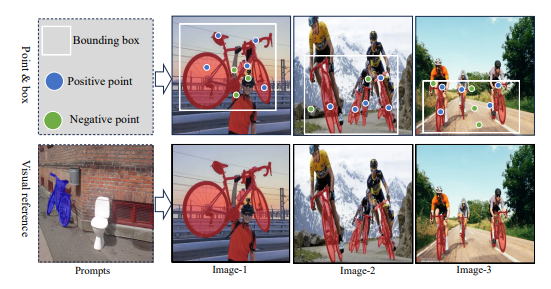
\includegraphics[width=1\linewidth]{VRP-SAM-1.png}%
    \caption{Comparison of SAM’s built-in Point and Box prompt modes with Visual Reference Prompt when handling numerous images. The prompts are all provided by users.}
    }
   
    \label{fig:VRP-SAM-1}
\end{figure}


\subsection{Architecture and Feature Augmentation}
VRP-SAM introduces a dedicated Visual Reference Prompt (VRP) encoder. It acts as a specialized intermediary, processing the support set and outputting tokens that mimic the mathematical behavior and dimensionality of SAM's native point prompts. 

However, relying solely on SAM's ViT encoder to extract features from the support image is problematic; SAM's features are highly geometric but semantically sparse. To prevent the frozen ViT from overlooking vital semantic details, the VRP encoder utilizes an auxiliary semantic-aware image encoder (typically a ResNet-50) to encode both the reference and target images into a shared, semantically rich latent space before prompt generation occurs.

\begin{figure}[htbp]
    \centering
    \IfFileExists{VRP-SAM-2.png}{%
        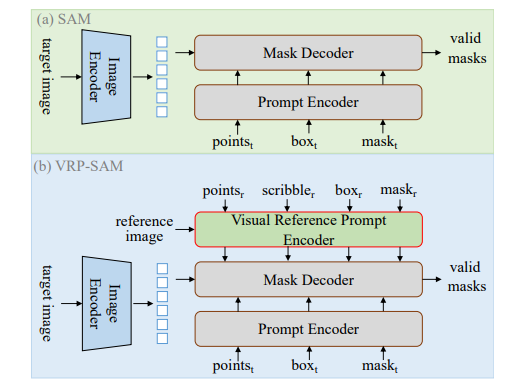
\includegraphics[width=1\linewidth]{VRP-SAM-2.png}%
        \caption{A Comparison between SAM and VRP-SAM. VRP-SAM introduces a visual reference prompt encoder, accepting annotated reference images with point, scribble, box, and mask formats, offering a distinct enhancement over SAM.}
    }
   
    \label{fig:VRP-SAM-2}
\end{figure}

\subsection{Mathematical Conditioning Mechanism}
The core adaptation logic in VRP-SAM relies on $N$ learnable query tokens, defined as $Q \in \mathbb{R}^{N \times C}$, where $C=256$ matches SAM's latent dimensionality. These queries are designed to aggregate the target's semantic information from the support image. They interact with the extracted reference features via a multi-head cross-attention mechanism. 

The attention operation is mathematically formulated as:
\begin{equation}
    P_{VRP} = \text{Softmax}\left(\frac{Q K_s^T}{\sqrt{d_k}}\right)V_s
\end{equation}
where $K_s$ and $V_s$ are the key and value projections generated from the foreground support features $F_s^{fg}$, and $d_k$ represents the scaling factor to prevent vanishing gradients during Softmax computation.

\begin{figure}[htbp]
    \centering
    \IfFileExists{VRP-SAM-3.png}{%
        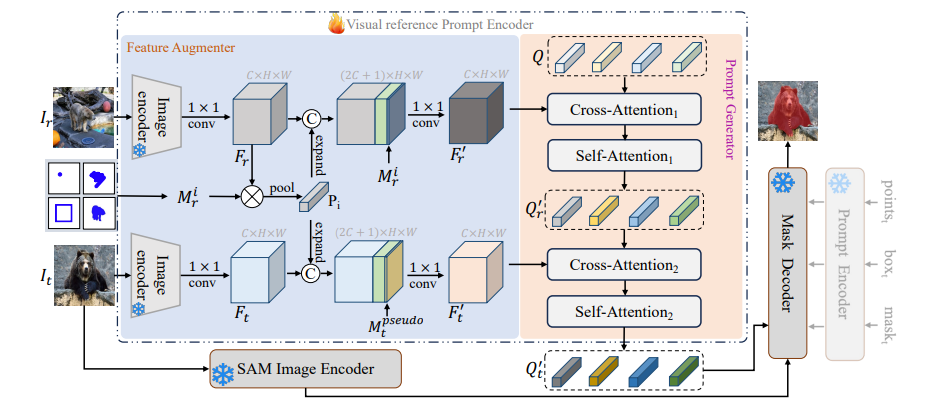
\includegraphics[width=1\linewidth]{VRP-SAM-3.png}%
        \caption{VRP-SAM framework. The approach enables SAM to perform visual reference segmentation by extends a VRP encoder. It takes various granularities of visual references as inputs and encodes these visual references into prompt embeddings. The VRP encoder consists of a feature augmenter and a prompt generator.}
    }
    
    \label{fig:VRP-SAM-3}
\end{figure}

\begin{algorithm}[H]
\caption{VRP-SAM Inference Pipeline}
\begin{algorithmic}[1]
\REQUIRE Support Image $I_s$, Support Mask $M_s$, Query Image $I_q$
\STATE Extract semantic features via auxiliary network: $F_s = \text{ResNet}(I_s)$, $F_q = \text{ResNet}(I_q)$
\STATE Apply binary mask $M_s$ to $F_s$ to explicitly isolate the target foreground: $F_s^{fg} = F_s \odot M_s$
\STATE Initialize $N$ learnable queries $Q$
\STATE Generate Visual Reference Prompt via Cross-Attention: $P_{VRP} = \text{CrossAttention}(Q, F_s^{fg}, F_s^{fg})$
\STATE Extract geometric query features via foundation model: $E_q = \text{SAM\_Encoder}(I_q)$
\STATE Predict High-Resolution Mask: $\hat{M}_q = \text{SAM\_Decoder}(E_q, P_{VRP})$
\RETURN $\hat{M}_q$
\end{algorithmic}
\end{algorithm}

\subsection{Strengths and Limitations}
\textbf{Strengths:} VRP-SAM establishes a highly computationally efficient baseline. Because the massive SAM backbone remains entirely frozen and the VRP encoder is relatively lightweight, it can process images at high FPS, making it suitable for real-time applications. It perfectly preserves SAM's native geometric boundary precision.\\
\textbf{Limitations:} The method is highly susceptible to prompt sensitivity. The deterministic, rigid nature of $P_{VRP}$ means that if the target object in the query image undergoes severe structural deformation (e.g., the articulation of a human body or the folding of a piece of clothing), the prompt embedding struggles to adapt to the new spatial reality, resulting in cascading decoder failures and fragmented mask outputs.

\newpage


\section{ProSAM: Probabilistic Prompting \cite{wang2025prosam}}

\subsection{Motivation}
Deterministic prompt generation, as utilized in VRP-SAM, is inherently brittle. SAM's mask decoder is highly non-linear; slight mathematical perturbations or variations in generated prompt tokens can cause the decoder to produce vastly different, often suboptimal, mask proposals. ProSAM fundamentally posits that modeling prompt uncertainty mathematically mitigates this instability. Unstable point prompts generated near the spatial boundaries of the target region are highly vulnerable to visual noise, whereas prompts generated near the object's center of mass yield much more robust segmentation.

\begin{figure}[htbp]
    \centering
    \IfFileExists{PRO-SAM-1.png}{%
        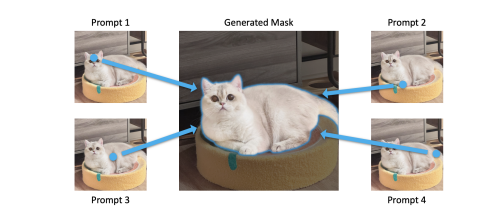
\includegraphics[width=1\linewidth]{PRO-SAM-1.png}%
        \caption{The same mask can be generated by SAM using various prompts in a region.}
    }
    
    \label{fig:PRO-SAM-1}
\end{figure}

\subsection{Variational Prompt Encoder and KL Divergence}
The core architectural innovation of ProSAM is the complete replacement of the deterministic encoder with a Variational Prompt Encoder. Utilizing principles from Variational Autoencoders (VAEs), it employs the reparameterization trick to model the prompt space as a continuous multivariate Gaussian distribution rather than a discrete point in latent space. 

Instead of a single discrete vector, the encoder predicts the mean vector $\mu$ and the covariance matrix $\Sigma$ of the target prompt embeddings. The model optimizes the Evidence Lower Bound (ELBO), explicitly minimizing the Kullback-Leibler (KL) divergence between the learned posterior distribution $q(Z|I_s, M_s)$ and a standard normal prior distribution $p(Z)$:
\begin{equation}
    \mathcal{L}_{KL} = D_{KL}(q(Z|I_s, M_s) || p(Z))
\end{equation}

\begin{figure}[htbp]
    \centering
    \IfFileExists{PRO-SAM-2.png}{%
        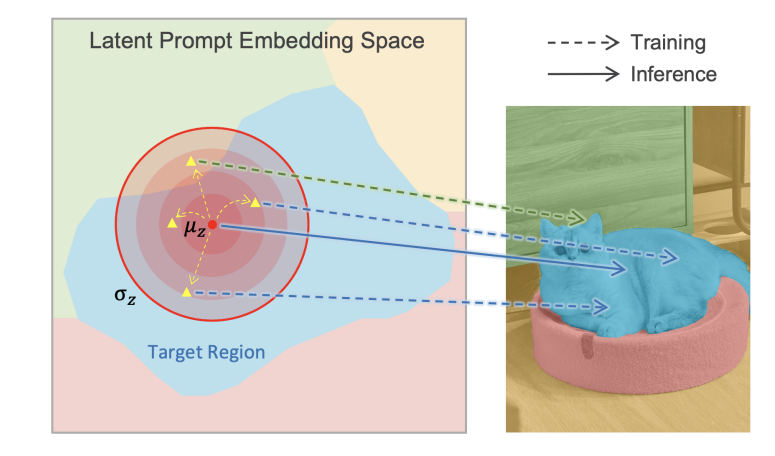
\includegraphics[width=0.75\linewidth]{PRO-SAM-2.png}%
         \caption{Intuitive illustration of the high-level idea behind the proposed variational prompt encoder. The dashed arrow shows the sampling and prompting procedure during training, while the solid arrow shows the prompting strategy during inference. Note that our generated prompts can be any type of prompt, while this illustration shows a positive point prompt as an example.}
    }
   
    \label{fig:PRO-SAM-2}
\end{figure}

\subsection{Probabilistic Conditioning and Laplacian Penalty}
During the mask generation phase at inference, ProSAM draws $K$ multiple prompt vector samples from the learned distribution $Z$. To optimally structure the latent space, it applies a geometric Laplacian penalty during meta-training. This penalty encourages the expected prompt embedding to reside in flatter, low-curvature regions of the loss landscape:
\begin{equation}
    \mathcal{L}_{Laplacian} = \lambda \sum_i \left| \nabla^2 \mathcal{L}_{CE}(\mu_i) \right|
\end{equation}
By strictly penalizing high-curvature regions, ProSAM structurally pushes the mean prompt $\mu$ toward the spatial center of the target region, safely away from ambiguous, noisy object boundaries.

\begin{figure}[htbp]
    \centering
    \IfFileExists{PRO-SAM-3.png}{%
        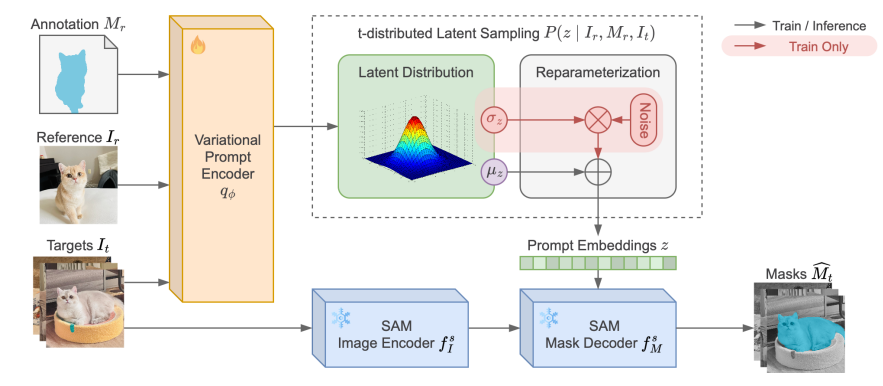
\includegraphics[width=1\linewidth]{PRO-SAM-3.png}%
         \caption{The overview of ProSAM, which segments the target images based on the visual references. Given a pre-trained SAM, a variational prompt encoder is trained to predict a multivariate prompt distribution with reparameterization trick. During the inference, the predicted mean prompt is employed to guide SAM in producing robust mask prediction for the target image.}
    }
  
    \label{fig:PRO-SAM-3}
\end{figure}

\begin{algorithm}[H]
\caption{ProSAM Probabilistic Inference Pipeline}
\begin{algorithmic}[1]
\REQUIRE Support $(I_s, M_s)$, Query $I_q$, Number of Monte Carlo Samples $K$
\STATE Predict distribution parameters: $\mu, \Sigma = \text{VariationalEncoder}(I_s, M_s)$
\STATE Extract high-resolution query features: $E_q = \text{SAM\_Encoder}(I_q)$
\FOR{$k = 1$ to $K$}
    \STATE Sample continuous prompt: $z_k = \mu + \epsilon_k \odot \Sigma^{1/2}, \quad \text{where } \epsilon_k \sim \mathcal{N}(0, I)$
    \STATE Predict candidate binary mask: $M_k = \text{SAM\_Decoder}(E_q, z_k)$
\ENDFOR
\STATE Marginalize geometric uncertainty by averaging candidates: $\hat{M}_q = \frac{1}{K} \sum_{k=1}^K M_k$
\RETURN Thresholded $\hat{M}_q$
\end{algorithmic}
\end{algorithm}

\subsection{Strengths and Limitations}
\textbf{Strengths:} ProSAM is exceptionally robust to boundary ambiguities and severe structural deformations. Marginalizing out prompt uncertainty yields stable predictions, making it particularly ideal for complex domains like medical imaging where tissue boundaries are inherently fuzzy.\\
\textbf{Limitations:} The necessity of sampling and processing multiple prompt candidates (requiring $K$ distinct, sequential passes through SAM's decoder network) substantially increases the overall computational overhead and inference latency, rendering it less suitable for high-speed video processing compared to deterministic methods.

\newpage


\section{Matcher: Feature Matching Approach \cite{liu2023matcher}}

\subsection{Motivation and Clarification}
Rather than compressing rich semantic information into SAM's extremely limited prompt dimensionality ($C=256$), Matcher \cite{liu2023matcher} leverages vision foundation models purely for dense feature extraction. \textbf{It is critical to clarify that Matcher is strictly an all-purpose feature matching framework, not a personalized segmentation model.} It strictly bypasses prompt engineering; it does not update foundation weights, nor does it train a task-specific meta-learner. It mathematically treats Few-Shot Segmentation purely as a dense coordinate-matching problem.

\begin{figure}[htbp]
    \centering
    \IfFileExists{MATCHER-1.png}{%
        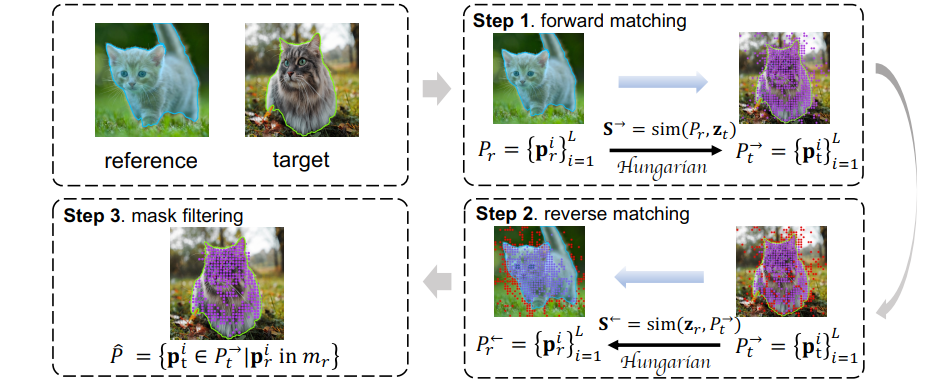
\includegraphics[width=1\linewidth]{MATCHER-1.png}%
        \caption{Illustration of the proposed bidirectional matching. Bidirectional matching consists of three steps: forward matching, reverse matching, and mask filtering. Purple points denote the matched points. Red points denote the outliers.}
    }
   
    \label{fig:MATCHER-1}
\end{figure}

\subsection{Dense Correlation and Bidirectional Matching}
Matcher utilizes a robust, self-supervised foundation model backbone (e.g., DINOv2 \cite{oquab2023dinov2}) to extract semantically meaningful, patch-level features. It constructs a dense correlation volume by computing the cosine similarity between every pixel in the query image $E_q \in \mathbb{R}^{H_q W_q \times C}$ and the foreground pixels in the support image $E_s^{fg} \in \mathbb{R}^{N_{fg} \times C}$:
\begin{equation}
    C_{i,j} = \frac{E_{q,i} \cdot E_{s,j}^{fg}}{||E_{q,i}|| ||E_{s,j}^{fg}||}
\end{equation}

To systematically eliminate matching outliers and visual hallucinations, Matcher employs a bidirectional matching strategy:
1. \textbf{Forward Matching:} Finds the coordinate with maximum similarity from the Reference domain to the Target domain.
2. \textbf{Reverse Matching:} Finds the coordinate with maximum similarity from the Target domain back to the Reference domain.

Only coordinates that are mutually agreed upon by both passes (cycle-consistent matches) are retained as valid, high-confidence spatial point prompts to be fed into SAM.

\subsection{Instance-Level Matching via Earth Mover's Distance}
Even with bidirectional filtering, SAM may output fragmented or false-positive masks when fed the selected point prompts. To suppress these, Matcher evaluates mask proposals using the Earth Mover's Distance (EMD). EMD computes the structural and spatial distance between the reference mask distribution $P$ and the query mask distribution $Q$:

\begin{equation}
    EMD(P, Q) = \frac{\min_{F=(f_{ij})} \sum_{i,j} f_{ij} d_{ij}}{\sum_{i,j} f_{ij}}
\end{equation}

By calculating the minimum cost to transform the query mask distribution into the support mask distribution, Matcher filters out highly divergent proposals, ensuring only structurally coherent masks are merged into the final output.

\begin{figure}[htbp]
    \centering
    \IfFileExists{MATCHER-2.png}{%
        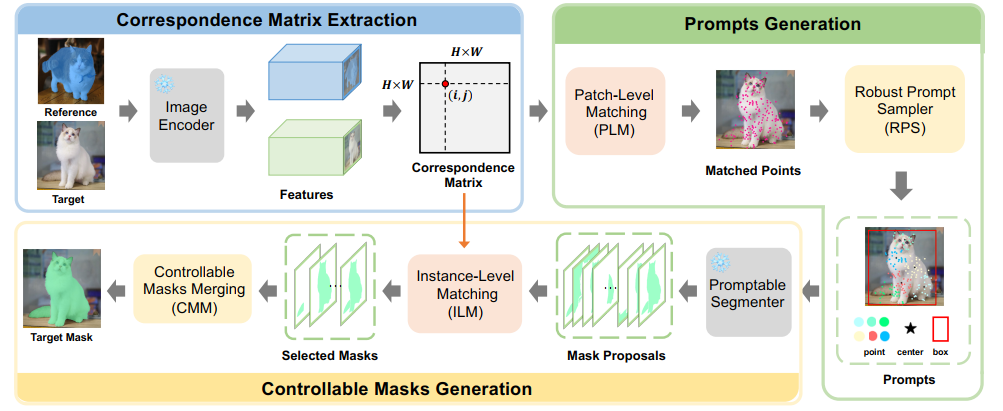
\includegraphics[width=1\linewidth]{MATCHER-2.png}%
        \caption{An overview of Matcher. The training-free framework addresses various segmentation tasks through three operations: Correspondence Matrix Extraction, Prompts Generation, and Controllable Masks Generation.}
    }
   
    \label{fig:MATCHER-2}
\end{figure}

\begin{algorithm}[H]
\caption{Matcher Feature Alignment Pipeline}
\begin{algorithmic}[1]
\REQUIRE Support $(I_s, M_s)$, Query $I_q$
\STATE Extract dense features: $E_s = \text{DINOv2}(I_s)$, $E_q = \text{DINOv2}(I_q)$
\STATE Extract foreground reference features: $E_s^{fg} = E_s \odot M_s$
\STATE Compute Correlation Matrix: $C_{sq} = E_s^{fg} \cdot E_q^T$
\STATE Filter matches via Bidirectional Check: $P_{coords} = \text{Bidirectional}(C_{sq})$
\STATE Feed verified coordinates as native points: $M_{candidates} = \text{SAM\_Decoder}(P_{coords})$
\STATE Evaluate candidates via $EMD(M_s, M_{candidate})$
\RETURN Merged true-positive masks $\hat{M}_q$
\end{algorithmic}
\end{algorithm}

\subsection{Strengths and Limitations}
\textbf{Strengths:} Matcher requires absolutely zero task-specific training or parameter updates, operating in a pure, elegant zero-shot paradigm. The methodology is highly interpretable.\\
\textbf{Limitations:} Matcher is highly prone to distractor suppression failures. If background elements in the query image share high feature similarity with the target object (e.g., segmenting a specific dog breed when multiple different dogs are in the background), the correlation volume inevitably generates false-positive spatial prompts that SAM will subsequently segment.

\newpage


\section{DC-SAM: Consistency-Based Adaptation \cite{qi2025dcsam}}

\subsection{Motivation}
In-context segmentation often suffers from semantic drift, where generated prompts fail to align precisely with the target class, drifting onto adjacent, visually similar objects during the decoding process. DC-SAM \cite{qi2025dcsam} addresses this by introducing cyclical validation to ensure rigorous semantic consistency between the initial reference intent and the final prediction.

\subsection{Dual-Consistency Mechanism and Cyclic Loss}
The architecture first fuses geometric features extracted by the frozen SAM encoder with semantic features obtained from a pre-trained auxiliary backbone. It implements a Cyclic Consistent Cross-Attention module. 

After generating an initial coarse mask $\hat{M}_{coarse}$, DC-SAM maps this segmentation output back into the prompt space, calculating the mathematical deviation $\Delta$ from the original reference intent:
\begin{equation}
    \mathcal{L}_{cyclic} = || P_{init} - \mathcal{F}_{reproject}(\hat{M}_{coarse}) ||_2^2
\end{equation}
Attention weights for cyclically inconsistent features are forced to negative infinity. This explicitly corrects semantic drift in real-time, heavily penalizing the network if the generated mask does not structurally match the initial visual prompt constraints.

\subsection{Positive and Negative Prompting}
DC-SAM fundamentally improves robustness by employing a dual-branch strategy. While most architectures solely extract discriminative positive prompts from the target foreground, DC-SAM explicitly utilizes the inverted background mask ($1 - M_s$) to generate explicit negative prompts. This dual representation pushes the latent embeddings of the target and background apart in the high-dimensional space, significantly enhancing discriminative power in cluttered scenes.

\begin{figure}[htbp]
    \centering
    \IfFileExists{DC-SAM-1.png}{%
        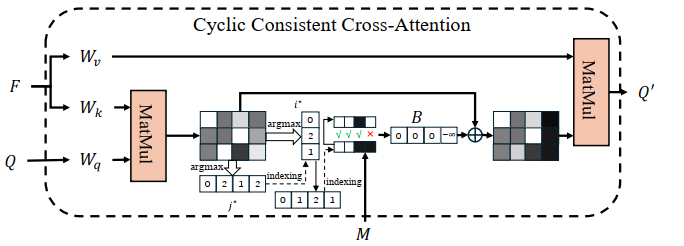
\includegraphics[width=1\linewidth]{DC-SAM-1.png}%
        \caption{Illustration of The proposed cyclic consistent cross-attention mechanism. This figure shows the version applied to query features with one head. The “Cyc” operation ultimately generates a bias to filter out features that are not cycle-consistent.}
    }
   
    \label{fig:DC-SAM-1}
\end{figure}

\begin{figure}[htbp]
    \centering
    \IfFileExists{DC-SAM-2.png}{%
        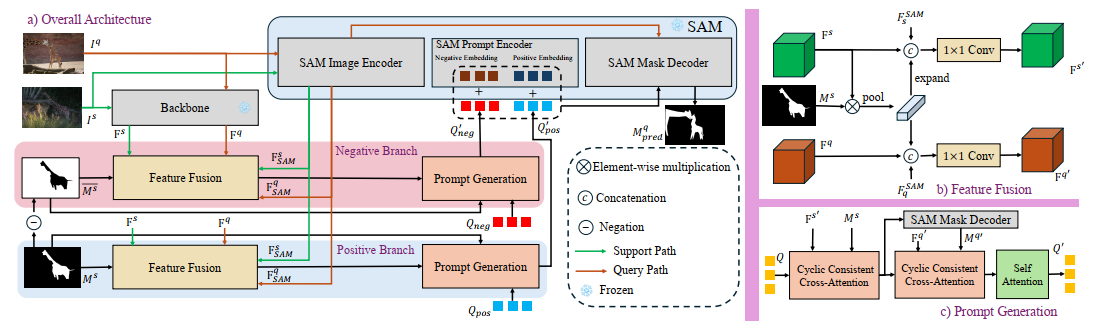
\includegraphics[width=1\linewidth]{DC-SAM-2.png}%
        \caption{Overview of the proposed DC-SAM framework. We use positive and negative branches to generate respective prompts, thereby refining the scope of the final generated mask. Additionally, we incorporate SAM features during the prompt generation process to better capture the characteristics of SAM, resulting in more accurate prompt boundaries. During the prompt generation process, we introduce cyclic consistent cross-attention to filter out non-cycle-consistent feature points, enhancing the precision of the prompts.}
    }
    
    \label{fig:DC-SAM-2}
\end{figure}

\begin{figure}[htbp]
    \centering
    \IfFileExists{DC-SAM-3.png}{%
        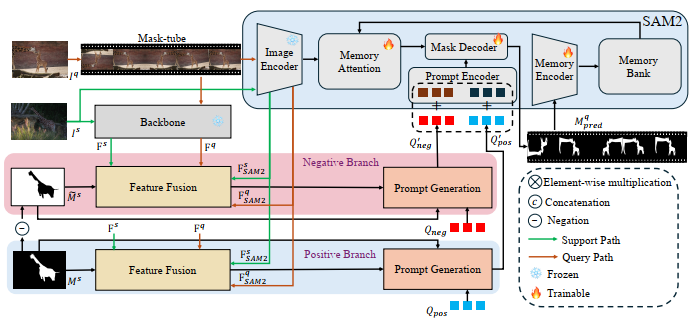
\includegraphics[width=1\linewidth]{DC-SAM-3.png}%
        \caption{Illustration of The proposed DC-SAM framework with SAM2 \cite{ravi2024sam2}. Unlike the image-level framework, we train the entire model for the video to acquire the image-to-video prompt ability. They apply different data augmentation techniques to the query image, and the augmented images compose a mask tube for training.}
    }
    
    \label{fig:DC-SAM-3}
\end{figure}

\begin{algorithm}[H]
\caption{DC-SAM Dual Consistency Loop}
\begin{algorithmic}[1]
\REQUIRE Support $(I_s, M_s)$, Query $I_q$
\STATE Extract Positive Prompts $P^+$ from $M_s$
\STATE Extract Negative Prompts $P^-$ from $(1 - M_s)$
\STATE Generate initial coarse prediction $\hat{M}_{coarse}$
\STATE Cyclic Check: Re-project $\hat{M}_{coarse}$ to prompt space $\hat{P}_{cyclic}$
\STATE Calculate consistency divergence: $\Delta = ||P^+ - \hat{P}_{cyclic}||_2$
\STATE Update Cross-Attention weights based on $\Delta$ (penalize high divergence)
\STATE Generate final mask $\hat{M}_q$ with updated attention constraints
\RETURN $\hat{M}_q$
\end{algorithmic}
\end{algorithm}

\subsection{Strengths and Limitations}
\textbf{Strengths:} DC-SAM exhibits exceptional distractor suppression capabilities. The explicit negative branching ensures strong generalization across both complex static images and continuous video domains (e.g., IC-VOS benchmark).\\
\textbf{Limitations:} The dual-branch architecture and recursive cyclic attention loops substantially increase the memory footprint and computational overhead, making it difficult to deploy on mobile or edge devices with restricted VRAM.

\newpage


\section{Bridge-the-Points: Graph-Based Reasoning  \cite{zhang2024bridge}}

\subsection{Motivation}
Dense clutter and multi-instance occlusion frequently confuse standard cross-attention mechanisms, which struggle to differentiate between adjacent, overlapping instances of the same object class. Bridge-the-Points \cite{zhang2024bridge} resolves this by mapping the spatial relationships within images as a topological graph, enabling advanced structural reasoning over semantic regions rather than relying on isolated pixel affinities.

\subsection{Graph-Based Prompt Generation and Adjacency}
The architecture utilizes a Positive-Negative Alignment (PNA) module to partition the pixel-wise correlation matrix into distinct foreground and background similarities, explicitly uncovering background context as negative references. Subsequently, a Point-Mask Clustering (PMC) module constructs a directed graph $\mathcal{G} = (\mathcal{V}, \mathcal{E})$. Vertices $\mathcal{V}$ represent selected points and their corresponding local masks, while edges $\mathcal{E}$ denote mask coverage over points. 

The adjacency matrix $A \in \mathbb{R}^{|\mathcal{V}| \times |\mathcal{V}|}$ defines the topological connections between spatial proposals. Vertices are clustered by identifying strongly connected components within the graph, effectively isolating the true target region from disconnected background noise.

\subsection{Structural Reasoning and Post-Gating}
To mitigate false positives, the method introduces strict post-gating strategies based on graph connectivity:
\begin{itemize}
    \item \textbf{Positive Gating:} Employs a mask growth algorithm evaluating pixel polarities to enforce spatial consistency.
    \item \textbf{Overshooting Gating:} Filters outlier points near object boundaries by measuring self-consistency between point features and the union mask of the connected component. If a predicted region lacks strong semantic edges connecting it back to the support nodes, the subgraph is severed and discarded entirely.
\end{itemize}

\subsection{Strengths and Limitations}
\textbf{Strengths:} A highly efficient, tuning-free pipeline that manages severe occlusion and complex background clutter through topological mathematics rather than brute-force feature matching. \\
\textbf{Limitations:} Constructing and traversing the directed graph scales poorly approaching $\mathcal{O}(|\mathcal{V}|^2)$ complexity with the number of generated candidate points. This introduces massive latency bottlenecks for high-resolution imagery where the candidate point subset exceeds thousands of nodes.

\begin{figure}[htbp]
    \centering
    \IfFileExists{BRIDGE-THE-POINTS-1.png}{%
        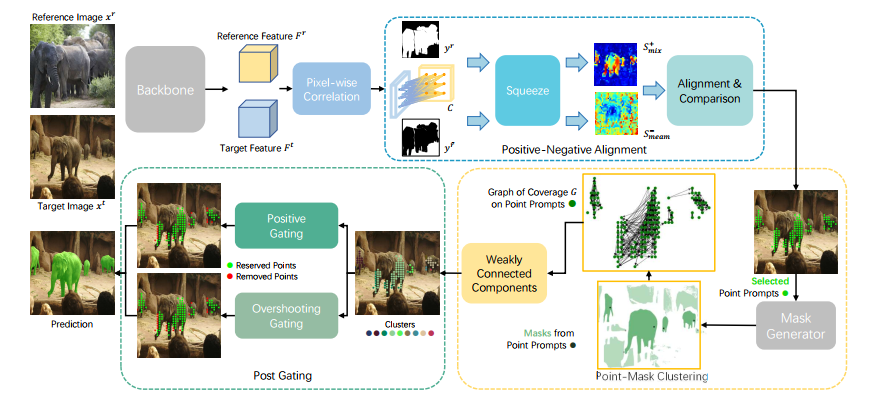
\includegraphics[width=1\linewidth]{BRIDGE-THE-POINTS-1.png}%
        \caption{Overview of The approach, where the Positive-Negative Alignment module recognizes the correlation between target features and reference features for point selection, the Point-Mask Clustering module efficiently clusters the points based on the coverage of corresponding masks, and Post-Gating filters out the false-positive masks for generating final prediction.}
    }
   
    \label{fig:BRIDE-THE-POINTS-1}
\end{figure}

\newpage


\section{FCP-SAM: Prototype-Based Modeling \cite{park2025fcpsam}}

\subsection{Motivation}
Discrete point and box prompts lack the capacity to convey complex, non-rigid object structures (e.g., fishing netting, smoke, complex biological forms like a spiderweb). FCP-SAM \cite{park2025fcpsam} abandons discrete geometric prompts, generating comprehensive, dense prototypes to guide the segmentation process via global feature modulation.

\begin{figure}[htbp]
    \centering
    \IfFileExists{FCP-SAM-1.png}{%
        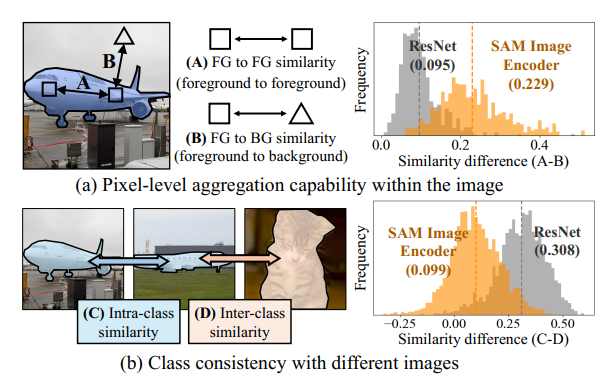
\includegraphics[width=1\linewidth]{FCP-SAM-1.png}%
        \caption{Comparison between ResNet and SAM Image Encoder features on 1000 PASCAL VOC images in test dataset, demonstrating their complementary strengths. (a) Similarity difference between FG-to-FG and FG-to-BG within the image. The higher similarity difference shown in SAM Image Encoder features reflects its superior pixel-level aggregation for prototype construction. (b) Difference between the FG-toFG similarity from the same class (intra-class) and different classes (inter-class). Compared to SAM features, ResNet features convey better class consistency across different images.}
    }
   
    \label{fig:FCP-SAM-1}
\end{figure}

\subsection{Foreground-Covering Prototype Generation}
FCP-SAM aggregates pixel-level features into dense, learnable tokens. It uniquely extracts SAM Image Encoder features for spatial granularity (taking advantage of SAM's high pixel-level similarity within instances) and couples them with auxiliary ResNet features to maintain rigid class consistency across vastly different query domains. 

Iterative cross-attention aggregates these disparate features into a comprehensive, unified prototype vector $p_c$:
\begin{equation}
    p_c = \frac{1}{\sum_{i,j} M_{s}(i,j)} \sum_{i,j} M_{s}(i,j) F_{s}(i,j)
\end{equation}
where $F_s$ represents the concatenated feature space.

\subsection{Prototype Matching and Attention Masks}
Instead of relying on rigid geometric pseudo-masks, FCP-SAM introduces a dynamic, attention-based pseudo-mask derived directly from the cross-attention weights. The final probability map is generated via prototype-to-prototype matching in the latent space, effectively avoiding the structural noise inherent in traditional prototype-to-pixel correlation techniques.

\begin{algorithm}[H]
\caption{FCP-SAM Prototype Matching}
\begin{algorithmic}[1]
\REQUIRE Support $(I_s, M_s)$, Query $I_q$
\STATE Extract geometric features: $G_s = \text{SAM\_Enc}(I_s)$, $G_q = \text{SAM\_Enc}(I_q)$
\STATE Extract semantic features: $S_s = \text{ResNet}(I_s)$, $S_q = \text{ResNet}(I_q)$
\STATE Generate Support Prototype $Proto_s$ via Iterative Cross-Attention
\STATE Predict query attention mask $\hat{A}_q$
\STATE Generate Query Prototype $Proto_q$ based on $\hat{A}_q$ and $S_q$
\STATE Calculate Cosine Similarity: $\mathcal{S}(Proto_s, Proto_q) = \frac{Proto_s \cdot Proto_q}{||Proto_s|| ||Proto_q||}$
\RETURN Final Mask $\hat{M}_q$ based on similarity score threshold
\end{algorithmic}
\end{algorithm}

\subsection{Strengths and Limitations}
\textbf{Strengths:} Exceptional global context modeling leading to excellent multi-shot scaling capability. Combining multi-shot prototypes mathematically via vector averaging is fundamentally more stable than combining discrete point coordinates.\\
\textbf{Limitations:} Reliance on a heavily parameterized auxiliary ResNet backbone for class consistency partially compromises the elegance, memory efficiency, and structural integrity of a pure, monolithic foundation model pipeline.

\begin{figure}[htbp]
    \centering
    \IfFileExists{FCP-SAM-2.png}{%
        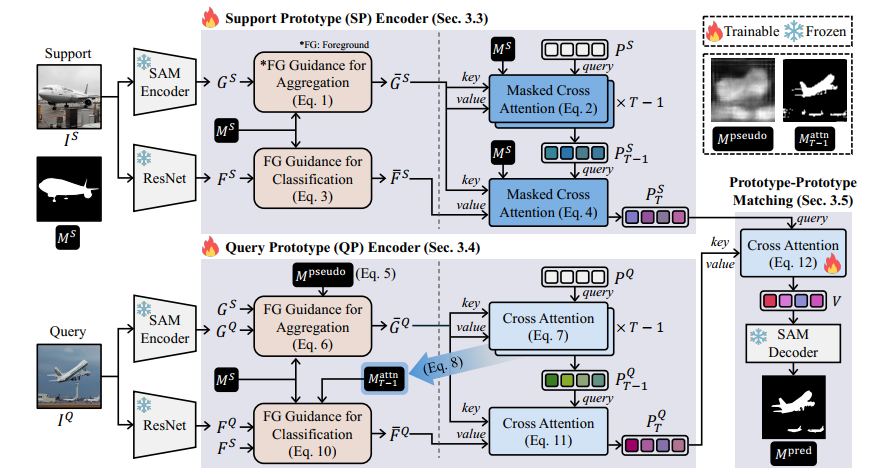
\includegraphics[width=1\linewidth]{FCP-SAM-2.png}%
        \caption{Overall pipeline of foreground-covering prototype generation and matching. Given SAM image encoder features, foreground regions are first highlighted using the support ground-truth mask and a pseudo mask for the query. The guided features are aggregated into learnable tokens via cross-attention. Since SAM features are not consistent across images, ResNet features are additionally used to provide class-consistent information. These ResNet features are guided by the support mask and an attention-based pseudo mask for the query to enhance foreground representation. The refined information is injected into the tokens to produce support and query prototypes. Finally, the query prototypes are matched with the support prototypes to form visual prompts, which are fed to the SAM decoder to predict the final query segmentation mask.}
    }
    
    \label{FCP-SAM-2.png}
\end{figure}

\newpage


\section{PerSAM: Personalized Few-Shot Segmentation \cite{zhang2024persam}}

\subsection{Motivation}
While foundational models like SAM demonstrate exceptional zero-shot capabilities, they fundamentally lack the ability to adapt to a user's specific, localized intent without continuous manual intervention. Personalizing SAM for a specific visual concept requires overcoming the model's generalized priors to focus exclusively on the specific visual characteristics of a user-provided target object. PerSAM (Personalize Segment Anything Model with One Shot) \cite{zhang2024persam} was developed to address this by introducing a training-free adaptation mechanism that guides SAM using only a single user-provided image and bounding box.

\subsection{Target-Guided Attention and Prompt Generation}
PerSAM operates by first extracting high-level semantic features from the user's reference image using SAM's pre-trained Vision Transformer backbone. It isolates the feature embedding of the target object utilizing the user-provided mask. 

When processing a new query image, PerSAM calculates the cosine similarity between every spatial feature vector in the query image and the reference target embedding. This dense correlation produces a target-guided spatial attention map. Instead of relying on random sampling or manual clicks, PerSAM autonomously selects the coordinates with the highest similarity scores as positive point prompts and the coordinates with the lowest similarity scores as negative point prompts. 

To refine the precise boundary delineation, the authors also proposed a fine-tuning variant (PerSAM-F). In this variant, the core foundation weights remain frozen, but a lightweight parameter-efficient fine-tuning (PEFT) mechanism is applied to the prompt encoder and mask decoder, optimizing them on the single available reference shot using a multi-scale regularization loss to preserve structural integrity.

\begin{figure}[htbp]
\centering
\IfFileExists{PerSAM-1.png}{%
    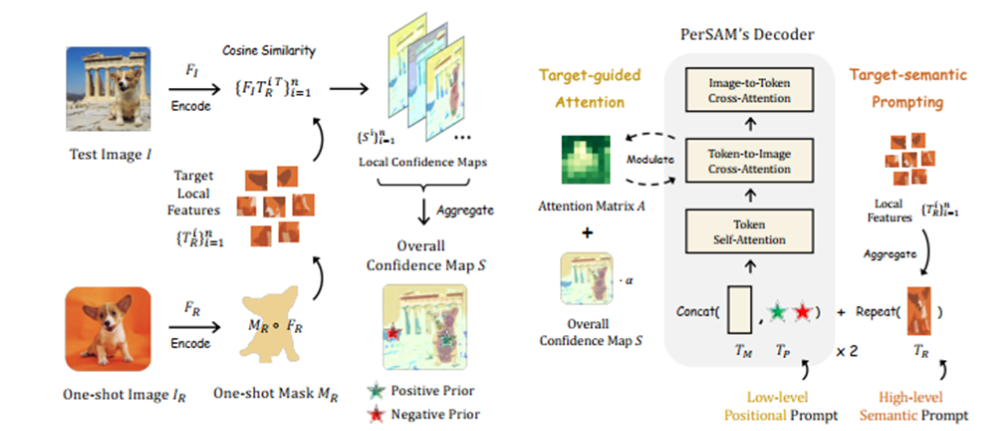
\includegraphics[width=1\linewidth]{PerSAM-1.png}%
    \caption{Positive-negative Location Prior.We calculate a location confidence map for the target object in new test image by the appearance of all local parts. Then, we select the location prior as the point prompt for PerSAM and Target-guided Attention (Left) \& Target-semantic Prompting (Right). To inject SAM with target semantics, we explicitly guide the cross-attention layers, and propose additional prompting with high-level cues.}
}

\label{fig:PerSAM-1}
\end{figure}


\begin{figure}[htbp]
\centering
\IfFileExists{PerSAM-2.png}{%
    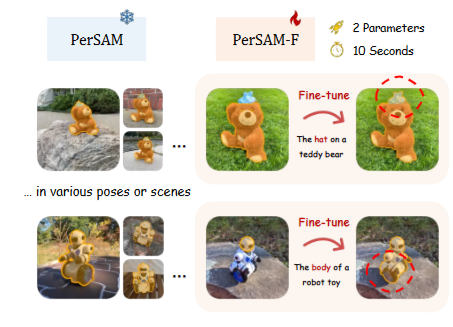
\includegraphics[width=0.5\linewidth]{PerSAM-2.png}%
    \caption{Personalized Segmentation Examples. PerSAM (Left) can segment personal
objects in any context with favorable performance, and PerSAM-F (right) further alleviates
the ambiguity issue by scale-aware fine-tuning.}
}

\label{fig:PerSAM-2}
\end{figure}

\begin{figure}[htbp]
\centering
\IfFileExists{PerSAM-3.png}{%
    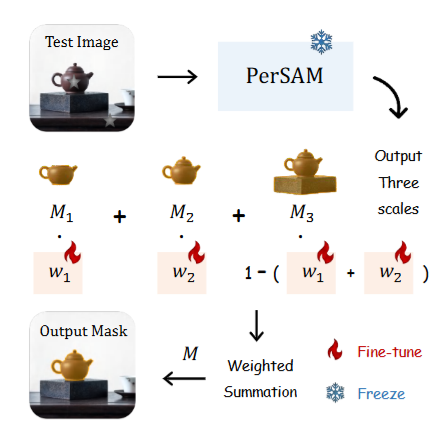
\includegraphics[width=0.5\linewidth]{PerSAM-3.png}%
    \caption{The Scale-aware Fine-tuning in
PerSAM-F. To alleviate the scale ambiguity,
PerSAM-F adopts two learnable weights for
adaptively aggregating three-scale masks.}
\label{fig:PerSAM-3}
\end{figure}
}



\subsection{Strengths and Limitations}
\textbf{Strengths:} The primary advantage of standard PerSAM is its complete lack of task-specific training, allowing for immediate, real-time personalization with minimal computational overhead. It demonstrates strong zero-shot transferability to video object segmentation tasks.\\
\textbf{Limitations:} The reliance on direct feature-level cosine similarity makes the training-free variant highly vulnerable to severe pose variations, extreme lighting changes, and intra-class variations where the query object's features diverge too far from the singular reference embedding.


\newpage


\section{DAPSAM: Domain Adaptation for Medical Segmentation \cite{wei2024prompting}}

\subsection{Motivation}
Applying generic visual foundation models to the medical domain presents a massive structural challenge. SAM is trained predominantly on natural images (SA-1B) characterized by sharp gradients, clear object boundaries, and high visual contrast. In stark contrast, medical imaging modalities (e.g., MRI, CT, ultrasound) frequently exhibit low contrast, ambiguous tissue boundaries, severe noise, and complex textural artifacts. Direct zero-shot application of SAM to medical datasets often results in catastrophic boundary failures and the oversegmentation of internal pathological structures. Domain-Adaptive Prototype SAM (DAPSAM) architectures \cite{wei2024prompting} directly address this fundamental domain gap. Crucially, DAPSAM tackles a challenge highly analogous to the core objectives of this doctoral research: Single-Source Domain Generalization (SDG). While our respective frameworks may diverge architecturally, the fundamental intersection between our work and DAPSAM lies predominantly in the specialized generation and adaptation of prompts specifically designed for the nuances of the medical domain.

\subsection{Domain-Adaptive Prompting Mechanisms}
DAPSAM frameworks operate by injecting domain-specific prior knowledge into the SAM architecture without fundamentally disrupting the frozen backbone's representational capacity. This is achieved through cross-domain feature alignment modules and specialized prompting mechanisms. 

Instead of relying solely on the raw geometric features extracted by SAM's generalized ViT, DAPSAM integrates a parallel medical-feature adaptation pathway that generates domain-adaptive prototypes. This pathway extracts domain-specific textures and pathological structures, projecting them into SAM's latent prompt space. By aligning the feature distributions between natural image priors and medical targets using contrastive or discrepancy-based loss functions, the model learns to generate prototypes that are specifically calibrated to detect fuzzy, low-contrast medical boundaries. Furthermore, DAPSAM architectures often incorporate uncertainty-aware bounding box generation to accommodate the inherent ambiguity of anatomical structures.

\begin{figure}[htbp]
\centering
\IfFileExists{DAPSAM.png}{%
    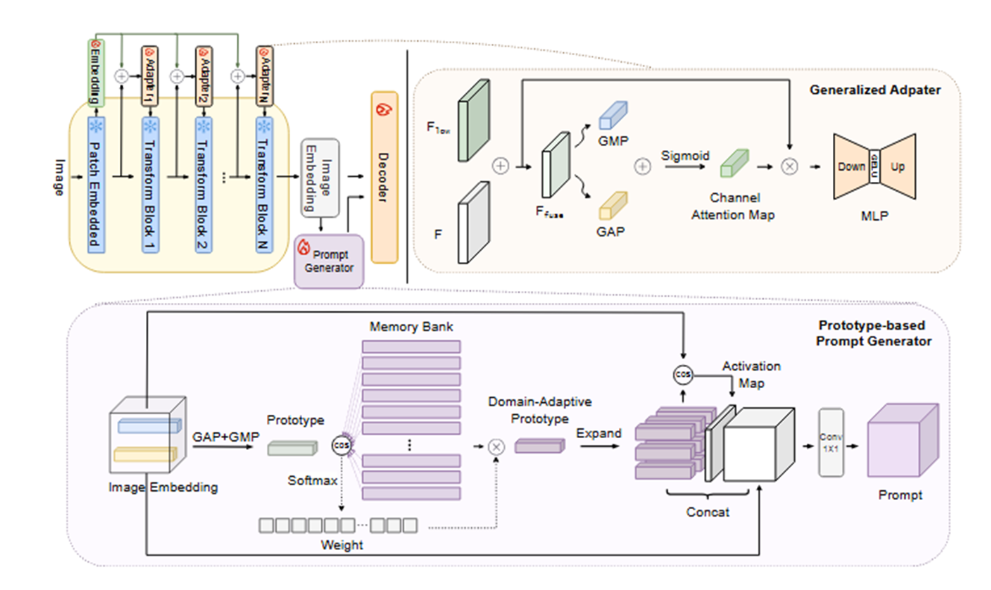
\includegraphics[width=1\linewidth]{DAPSAM.png}%
    \caption{The pipeline of the proposed DAPSAM. a generalization framework is designed to fine-tune SAM, with generalized adapters (top right) to obtain robust features and a prompt generation module (bottom) to generate instance-related source domain prototypes for target image segmentation.}
}

\label{fig:DAPSAM}
\end{figure}

\subsection{Strengths and Limitations}
\textbf{Strengths:} DAPSAM bridges the critical gap between natural image pre-training and clinical applicability, substantially outperforming vanilla SAM on challenging clinical benchmarks (such as tumor delineation or organ segmentation) without requiring the massive dataset sizes typically needed to train specialized medical networks from scratch.\\
\textbf{Limitations:} Developing robust cross-domain alignment requires access to representative, high-quality medical datasets during the meta-training phase. Additionally, the domain-adaptive modules introduce further computational latency, which can hinder deployment in highly constrained, real-time clinical diagnostic hardware.

% ==========================================
% CHAPTER 3: BENCHMARKING , EVALUATION METRICS and COMPARITIVE RESULTS
% ==========================================
\chapter{Benchmarking, Evaluation Metrics, and Comparative Results}

\section{Dataset Descriptions and Challenge Parameters}
To provide a highly rigorous, comprehensive evaluation of the foundation models' generalization limits, experiments are synthesized across distinct datasets. These datasets are strategically categorized into testing domains: standard baselines (assessing core object extraction and distractor suppression), large-vocabulary benchmarks (pushing the limits of open-set scalability), part-level semantics (evaluating high-resolution intra-object reasoning), personalized segmentation, and medical domain generalization.

\subsection{Standard Baselines}
\begin{itemize}
    \item \textbf{PASCAL-$5^i$ \cite{shaban2017one}:} Derived from the PASCAL VOC 2012 \cite{everingham2010pascal} and Semantic Boundaries Dataset (SBD). It contains 20 object categories divided evenly across 4 cross-validation folds. 
    \textbf{Visual Characteristics:} Images typically feature centered, single-dominant foreground objects with moderate occlusion and relatively low background clutter. 
    \textbf{Evaluation Role:} Serves as the standard baseline entry-point, primarily measuring basic foreground extraction precision and rudimentary semantic alignment.
    
    \item \textbf{MS COCO-$20^i$ \cite{nguyen2019feature}:} Derived from the MS COCO dataset \cite{lin2014microsoft}, this benchmark introduces a massive step up in structural complexity. It encompasses 80 diverse categories split into 4 testing folds. 
    \textbf{Visual Characteristics:} Presents highly challenging scenes filled with dense multi-instance clutter, severe scale variation, and heavy subject occlusion. 
    \textbf{Evaluation Role:} Serves as the primary ``Distractor Challenge,'' rigorously testing a model's capacity to suppress visually similar background elements and maintain accurate correspondence under chaotic contextual interference.
\end{itemize}

\subsection{Large-Vocabulary Benchmarks}
\begin{itemize}
    \item \textbf{FSS-1000 \cite{li2020fss}:} Designed explicitly to benchmark the limits of few-shot learning systems, containing 10,000 images spanning exactly 1,000 distinct, fine-grained categories.
    \textbf{Visual Characteristics:} Focuses on rare or unconventional objects (e.g., obscure items, specific logos, specialized merchandise) presented against relatively clean backgrounds.
    \textbf{Evaluation Role:} Evaluates extreme open-set generalization on entities entirely absent from standard foundation model pre-training distributions.
    
    \item \textbf{LVIS-$92^i$ \cite{gupta2019lvis}:} Derived from the Large Vocabulary Instance Segmentation benchmark, representing the upper bound of modern semantic complexity with a severe long-tailed distribution exceeding 1,200 unique categories.
    \textbf{Visual Characteristics:} Contains extremely rare entities embedded inside highly complex and varied spatial layouts.
    \textbf{Evaluation Role:} Acts as the ultimate scalability test, evaluating structural robustness against extreme data imbalance and the model's ability to avoid defaulting to common geometric priors.
\end{itemize}

\subsection{Part-Level Semantics}
\begin{itemize}
    \item \textbf{PASCAL-Part \cite{chen2014detect}:} A high-resolution, fine-grained extension of the foundational PASCAL VOC dataset. It shifts the task definition from bounding entire objects to identifying specific anatomical or structural parts.
    \textbf{Visual Characteristics:} Target regions frequently possess minimal visual contrast against adjacent sub-parts (e.g., separating a dog's leg from its torso).
    \textbf{Evaluation Role:} Validates the network's capacity for high-resolution, intra-object geometric localization.
    
    \item \textbf{PACO-Part \cite{ramanathan2023paco}:} The Parts and Attributes of Common Objects dataset provides unparalleled semantic depth, spanning 75 distinct object categories subdivided into over 200 diverse part categories.
    \textbf{Visual Characteristics:} Features highly complex contextual interactions and ambiguous object-part compositions.
    \textbf{Evaluation Role:} Serves as a rigorous evaluation of fine-grained structural reasoning, ensuring models establish true semantic correspondences rather than relying on coarse visual proxies.
\end{itemize}

\subsection{Personalized and Video Segmentation}
\begin{itemize}
    \item \textbf{PerSeg \cite{zhang2024persam}:} A specialized dataset constructed explicitly to evaluate one-shot personalized object segmentation.
    \textbf{Visual Characteristics:} Contains diverse images of specific user-designated personal objects (e.g., a specific pet dog, a personal backpack, a unique toy) captured across radically different contexts, backgrounds, and poses.
    \textbf{Evaluation Role:} Shifts the evaluation paradigm from generic category-level recognition (e.g., finding "any dog") to strict instance-level fidelity (e.g., finding "this exact dog"), testing the model's ability to resist semantic drift.
    
    \item \textbf{DAVIS 2017 \cite{pont2017the}:} The Densely Annotated VIdeo Segmentation benchmark. 
    \textbf{Visual Characteristics:} Contains high-quality, full-HD video sequences featuring complex object deformations, heavy occlusions, motion blur, and chaotic background distractors.
    \textbf{Evaluation Role:} Used to evaluate the zero-shot temporal transfer capabilities of personalized models (e.g., PerSAM), testing whether a single static reference frame can guide segmentation across a continuous, dynamic video sequence without temporal retraining.
\end{itemize}

\subsection{Medical Domain Generalization}
\begin{itemize}
    \item \textbf{Multi-Center Prostate MRI \& Fundus Benchmarks \cite{wei2024prompting}:} Representative medical imaging datasets used to evaluate single-source domain generalization (SDG). The Prostate dataset includes multi-center MRI scans for prostate segmentation. The RIGA+ Fundus dataset includes retinal images from multiple centers (BinRushed, Magrabia) for Optic Disc and Cup segmentation.
    \textbf{Visual Characteristics:} Characterized by severe domain shifts caused by different scanner vendors, inherent low-contrast tissue boundaries, and heavy noise typical of clinical environments.
    \textbf{Evaluation Role:} Rigorously tests the model's capacity to override natural-image geometric priors and adapt to ambiguous, low-contrast clinical structures without catastrophic failure.
\end{itemize}

\section{Evaluation Protocol}
Models are rigorously evaluated using the mean Intersection over Union (mIoU) metric for static images, calculated over cross-validation folds:
\begin{equation}
    mIoU = \frac{1}{C} \sum_{c=1}^C \frac{TP_c}{TP_c + FP_c + FN_c}
\end{equation}
where $C$ is the number of classes, and $TP, FP, FN$ denote true positives, false positives, and false negatives, respectively. 

For medical segmentation tasks, the Dice Similarity Coefficient (DSC), also referred to as the Dice Score, is utilized to measure the spatial overlap between the predicted segmentation $X$ and the ground truth $Y$:
\begin{equation}
    DSC = \frac{2 |X \cap Y|}{|X| + |Y|}
\end{equation}
The Dice score is particularly effective for evaluating medical structures, where true negative background pixels heavily outnumber foreground target pixels. Optic Disc Overlap Dice (DOD) and Optic Cup Overlap Dice (DOC) are specific applications of this metric.

For video object segmentation (VOS) tasks, such as those evaluated on the DAVIS 2017 benchmark, performance is quantified using **Region Similarity ($\mathcal{J}$)** and **Boundary Accuracy ($\mathcal{F}$)**.

The Region Similarity ($\mathcal{J}$), mathematically equivalent to the Intersection over Union (IoU), measures the spatial overlap between the predicted segmentation mask $M$ and the ground-truth mask $G$:
\begin{equation}
    \mathcal{J} = \frac{|M \cap G|}{|M \cup G|}
\end{equation}

The Boundary Accuracy ($\mathcal{F}$) evaluates the structural integrity of the segmented object's contours. It is defined as the harmonic mean of the contour precision ($P_c$) and contour recall ($R_c$):
\begin{equation}
    \mathcal{F} = \frac{2 \cdot P_c \cdot R_c}{P_c + R_c}
\end{equation}

To compute $P_c$ and $R_c$, let $\mathcal{S}_M$ and $\mathcal{S}_G$ represent the sets of boundary points for the predicted mask and ground truth, respectively. Given a spatial distance threshold $\epsilon$, the metrics are formulated as follows:
\begin{itemize}
    \item \textbf{Contour Precision ($P_c$):} The proportion of points in the predicted boundary that lie within a distance $\epsilon$ of the ground-truth boundary:
    \begin{equation}
        P_c = \frac{|\{p \in \mathcal{S}_M \mid d(p, \mathcal{S}_G) < \epsilon\}|}{|\mathcal{S}_M|}
    \end{equation}
    
    \item \textbf{Contour Recall ($R_c$):} The proportion of points in the ground-truth boundary that lie within a distance $\epsilon$ of the predicted boundary:
    \begin{equation}
        R_c = \frac{|\{p \in \mathcal{S}_G \mid d(p, \mathcal{S}_M) < \epsilon\}|}{|\mathcal{S}_G|}
    \end{equation}
\end{itemize}
where $d(p, \mathcal{S})$ denotes the minimum Euclidean distance from point $p$ to the nearest point in set $\mathcal{S}$. In standard evaluation protocols, $\epsilon$ is typically set to $0.0075$ times the image diagonal. The final performance is reported as the global mean $\mathcal{J}\&\mathcal{F}$.

\section{Standard and Large-Vocabulary Few-Shot Segmentation}

\noindent\textbf{Evaluation Protocol.}
To comprehensively assess the effectiveness of recent reference-guided few-shot segmentation methods, we evaluate performance across both standard and large-vocabulary benchmarks that exhibit complementary characteristics. The selected datasets include PASCAL-$5^i$, COCO-$20^i$, FSS-1000, and LVIS-$92^i$, which collectively cover a wide spectrum of scene complexity, object diversity, and distractor density. Performance is measured using mean Intersection-over-Union (mIoU), the standard metric for few-shot segmentation, under both 1-shot and 5-shot settings. This multi-dataset evaluation protocol enables a rigorous analysis of each method’s ability to generalize from limited reference examples while maintaining robustness to clutter, semantic diversity, and long-tail category distributions. 

The quantitative results extracted from the evaluated methodologies are presented in Table \ref{tab:results_overall}. 

\begin{table}[htbp]
\centering
\caption{Overall Quantitative Results (mIoU \%) on Standard and Large-Vocabulary Datasets}
\label{tab:results_overall}
\resizebox{\linewidth}{!}{
\begin{tabular}{l l c c c c c c c c}
\toprule
\textbf{Method} & \textbf{Backbone} & \multicolumn{2}{c}{\textbf{PASCAL-5i}} & \multicolumn{2}{c}{\textbf{COCO-20i}} & \multicolumn{2}{c}{\textbf{FSS-1000}} & \multicolumn{2}{c}{\textbf{LVIS-92i}} \\
\cmidrule(lr){3-4} \cmidrule(lr){5-6} \cmidrule(lr){7-8} \cmidrule(lr){9-10}
& & \textbf{1-s} & \textbf{5-s} & \textbf{1-s} & \textbf{5-s} & \textbf{1-s} & \textbf{5-s} & \textbf{1-s} & \textbf{5-s} \\
\midrule
VRP-SAM \cite{sun2024vrp} & ResNet-50 & 71.9 & 72.9 & 53.9 & -- & -- & -- & -- & -- \\
VRP-SAM \cite{sun2024vrp} & DINOv2 & -- & -- & 60.4 & -- & -- & -- & -- & -- \\
ProSAM \cite{wang2025prosam} & ResNet-50 & 72.04 & -- & 54.63 & -- & -- & -- & -- & -- \\
ProSAM \cite{wang2025prosam} & DINOv2 & -- & -- & 59.16 & -- & -- & -- & -- & -- \\
Matcher \cite{liu2023matcher} & DINOv2 & -- & -- & 52.7 & 60.7 & 87.0 & 89.6 & 33.0 & 40.0 \\
DC-SAM \cite{qi2025dcsam} & ResNet-50 & 73.0 & -- & 55.5 & -- & -- & -- & -- & -- \\
DC-SAM \cite{qi2025dcsam} & DINOv2 & -- & -- & 62.0 & -- & -- & -- & -- & -- \\
DC-SAM (SAM2) \cite{qi2025dcsam},\cite{ravi2024sam2} & ResNet-50 & 74.0 & -- & 56.4 & -- & -- & -- & -- & -- \\
Bridge-the-Points \cite{zhang2024bridge} & DINOv2 & 72.1 & 82.6 & 58.7 & 66.8 & 88.0 & 88.9 & 35.2 & 44.2 \\
FCP-SAM \cite{park2025fcpsam} & ResNet-50 & 73.2 & 74.0 & 52.5 & 58.0 & -- & -- & -- & -- \\
\bottomrule
\multicolumn{10}{l}{\small \textit{*Note: Missing values indicate the metric was not explicitly reported in the primary study.}}
\end{tabular}}
\end{table}

\noindent\textbf{Overall Analysis and Takeaway.}
The cross-benchmark evaluation reveals that each dataset emphasizes a distinct aspect of reference-guided few-shot segmentation. PASCAL-$5^i$ primarily measures precise foreground extraction in scenes with a dominant object and limited distractors, leading to relatively small performance gaps between methods. COCO-$20^i$ introduces dense clutter and multiple co-occurring objects, thereby evaluating the ability to suppress distractors and maintain accurate correspondence under complex context. LVIS-$92^i$ constitutes the most challenging large-vocabulary setting, characterized by rare categories and long-tail distributions, testing scalability to extreme semantic diversity. FSS-1000, in contrast, assesses generalization across a large number of categories with comparatively clean scenes, emphasizing category-level transfer rather than distractor robustness.

The quantitative results reflect these evaluation objectives. Methods based on consistency enforcement achieve the strongest performance on COCO-$20^i$ in the 1-shot regime, while graph-based reasoning demonstrates superior scalability on LVIS-$92^i$ and clear benefits in multi-shot settings, where relational modeling across support examples becomes increasingly important. On PASCAL-$5^i$, several approaches achieve comparable performance, indicating that simpler scenes reduce sensitivity to methodological differences.

A consistent trend across methods reporting multiple backbones is the superiority of DINOv2 over ResNet-50. Substantial gains are observed when replacing convolutional features with self-supervised transformer representations. As explicitly detailed in Table~\ref{tab:backbone_comp}, improvements include jumping from 53.9\% to 60.4\% for VRP-SAM, 54.63\% to 59.16\% for ProSAM, and 55.5\% to 62.0\% for DC-SAM on the highly cluttered COCO-$20^i$ dataset. This pattern highlights the critical role of representation quality, suggesting that foundation-model encoders provide vastly more transferable semantic features for reference-guided segmentation tasks.

\begin{table}[htbp]
\centering
\caption{Impact of Backbone Choice on COCO-$20^i$ (1-Shot mIoU \%)}
\label{tab:backbone_comp}
\begin{tabular}{l c c c}
\toprule
\textbf{Method} & \textbf{ResNet-50} & \textbf{DINOv2} & \textbf{Absolute Gain} \\
\midrule
VRP-SAM \cite{sun2024vrp} & 53.90 & 60.40 & +6.50 \\
ProSAM \cite{wang2025prosam} & 54.63 & 59.16 & +4.53 \\
DC-SAM \cite{qi2025dcsam} & 55.50 & 62.00 & +6.50 \\
\bottomrule
\end{tabular}
\end{table}

Collectively, these findings demonstrate that current methods exhibit dataset-dependent strengths and lack uniform robustness across varying levels of clutter, vocabulary size, and scene complexity. This inconsistency exposes a fundamental limitation of existing approaches and underscores the necessity for segmentation frameworks that integrate strong foundation-model representations with adaptive reasoning mechanisms capable of maintaining stable performance across both standard and large-vocabulary scenarios.

\section{One-shot Object Part Segmentation}
One-shot object part segmentation requires identifying and delineating semantic parts of an object (e.g., wheel, head, wing) from a single annotated reference example. Compared to whole-object segmentation, this task demands substantially finer-grained understanding, as the model must capture subtle intra-object boundaries, handle strong visual similarity between adjacent parts, and generalize part semantics across varying object poses and appearances.

PASCAL-Part and PACO-Part constitute challenging benchmarks for this setting, each emphasizing different aspects of fine-grained reasoning. PASCAL-Part focuses on structured part decomposition of common object categories, testing the ability to localize well-defined components under moderate variation. PACO-Part, in contrast, introduces greater diversity in object-part compositions and more complex contextual interactions, thereby evaluating robustness to higher semantic granularity and ambiguity.

The quantitative results in Table~\ref{tab:part_seg} indicate that both evaluated methods achieve substantially lower mIoU compared to whole-object segmentation benchmarks, confirming the increased difficulty of part-level reasoning. Bridge-the-Points achieves the best performance on both datasets, attaining 44.5\% on PASCAL-Part and 36.3\% on PACO-Part, outperforming Matcher by margins of 1.6 and 1.6 percentage points, respectively. This consistent improvement suggests that modeling structural relationships between regions is particularly beneficial for capturing fine-grained part correspondences, where simple feature matching may struggle to disambiguate visually similar components.

Overall, the relatively low absolute performance across methods highlights one-shot part segmentation as an open challenge for reference-guided segmentation frameworks, underscoring the need for approaches capable of integrating precise localization with robust semantic reasoning at the intra-object level.

\begin{table}[htbp]
\centering
\caption{Results (mIoU \%) on One-Shot Part Segmentation Datasets}
\label{tab:part_seg}
\begin{tabular}{l c c}
\toprule
\textbf{Method} & \textbf{PASCAL-Part (1-shot)} & \textbf{PACO-Part (1-shot)} \\
\midrule
Matcher \cite{liu2023matcher} & 42.9 & 34.7 \\
Bridge-the-Points \cite{zhang2024bridge} & 44.5 & 36.3 \\
\bottomrule
\end{tabular}
\end{table}

\section{Personalized and Domain-Adaptive Segmentation}

While standard benchmarks evaluate generalization across generic categories, personalized and medical applications demand extreme specialization from a single reference image, presenting unique structural challenges for foundation models.

\noindent\textbf{Personalized Segmentation (PerSAM):}
Evaluating PerSAM on the PerSeg dataset highlights the power of target-guided attention combined with parameter-efficient fine-tuning. As shown in Table \ref{tab:persam_results}, the training-free variant of PerSAM achieves strong baseline personalization with an mIoU of 89.3\%. Furthermore, the fine-tuned variant (PerSAM-F)—which optimizes merely 2 scale-aware parameters within 10 seconds—achieves a remarkable mIoU of 95.3\% on the PerSeg benchmark, bypassing the need for heavy structural retraining.

To test temporal robustness, PerSAM was additionally evaluated on the \textbf{DAVIS 2017} video object segmentation benchmark using a strictly zero-shot, frame-by-frame approach. Guided by only the first annotated frame, PerSAM-F maintains high fidelity across dynamic sequences, achieving highly competitive Region Similarity and Boundary Accuracy ($\mathcal{J}\&\mathcal{F}$) metrics (76.1\%). This proves that precise spatial personalization can successfully override temporal motion blur and deformation artifacts without complex temporal cross-attention layers.

\begin{table}[htbp]
\centering
\caption{Quantitative Results on Personalized and Video Segmentation}
\label{tab:persam_results}
\begin{tabular}{l l c c}
\toprule
\textbf{Method} & \textbf{Adaptation Type} & \textbf{PerSeg (mIoU \%)} & \textbf{DAVIS 2017 ($\mathcal{J}\&\mathcal{F}$ \%)} \\
\midrule
PerSAM \cite{zhang2024persam} & Training-Free & 89.3 & 66.9 \\
PerSAM-F \cite{zhang2024persam} & PEFT (2 parameters) & 95.3 & 76.1 \\
\bottomrule
\end{tabular}
\end{table}

\noindent\textbf{Medical Domain Generalization (DAPSAM):}
In the clinical domain, the zero-shot application of generic foundation models routinely fails due to the semantic-geometric gap between natural images and medical scans. Evaluations of DAPSAM on multi-center Prostate MRI and Optic Cup/Disc Fundus datasets demonstrate that standard cross-attention adapters are insufficient for handling severe domain shifts. 

As detailed in Table \ref{tab:dapsam_results}, standard SAM suffers from catastrophic boundary failure on low-contrast medical targets. By employing a learnable memory bank to construct domain-adaptive prototypes, DAPSAM significantly outperforms vanilla SAM, achieving a state-of-the-art Dice Similarity Coefficient (DSC) of 88.6\% for Prostate segmentation. The explicit alignment of low-level and intermediate features allows DAPSAM to parse fuzzy, clinical boundaries that cause standard decoders to fail, establishing a robust framework for prompt-driven medical segmentation.

\begin{table}[htbp]
\centering
\caption{Domain Generalization Results on Medical Datasets (Dice Score \%)}
\label{tab:dapsam_results}
\resizebox{\linewidth}{!}{ % Optional: ensures the table fits the page width
\begin{tabular}{l l c c c} % Updated to 5 columns
\toprule
\textbf{Method} & \textbf{Adaptation Mechanism} & \textbf{Prostate MRI} & \textbf{RIGA+ (DOD)} & \textbf{RIGA+ (DOC)} \\
\midrule
DAPSAM \cite{wei2024prompting} & Domain-Adaptive Prototypes & 81.31 & 96.30 & 88.15 \\
\bottomrule
\end{tabular}
}
\end{table}


% ==========================================
% CHAPTER 4: TECHNICAL DISCUSSION
% ==========================================
\chapter{Technical Discussion}

\section{The Necessity of Explicit Semantic Alignment}
The empirical results across standard, large-vocabulary, and part-level benchmarks consistently demonstrate that SAM's native geometric prompting mechanisms are insufficient for reliable reference-guided segmentation without additional semantic alignment. While point, box, or mask prompts provide coarse localization cues, they lack the capacity to encode category-level semantics or disambiguate visually similar regions. This limitation becomes particularly evident on COCO-$20^i$ and LVIS-$92^i$, where dense distractors and long-tail categories require precise semantic correspondence rather than geometric proximity. Methods incorporating explicit alignment mechanisms such as prototype aggregation, graph-based relational reasoning, or cyclic consistency enforcement consistently outperform simple prompt-based approaches under these challenging conditions.

The necessity of semantic alignment is further reinforced by results on one-shot part segmentation datasets, where fine-grained intra-object boundaries must be distinguished despite minimal visual contrast between adjacent parts. The relatively low performance across methods on PASCAL-Part and PACO-Part indicates that geometric cues alone cannot capture subtle semantic distinctions within objects. Effective segmentation therefore requires mechanisms that explicitly map support features to query representations at the semantic level, preventing the model from defaulting to visually salient but irrelevant regions.

\section{Methodological Insights on Negative Prompting}
A consistent source of performance improvement across evaluated methods is the incorporation of explicit negative prompting, which leverages background regions as informative counterexamples. By treating non-target regions in the support image as negative references, models can better resolve ambiguities between the target object and visually similar distractors. This strategy proves particularly effective on cluttered datasets such as COCO-$20^i$ and LVIS-$92^i$, where background objects often share textures, colors, or shapes with the target category.

Negative prompting also contributes to stability in multi-shot scenarios by preventing overfitting to dominant foreground patterns in the support set. Without explicit suppression of background features, models may incorrectly segment salient but irrelevant regions, especially when support examples are limited. These findings indicate that modeling both positive correspondences and negative constraints is essential for robust reference-guided segmentation.

\section{Impact of Representation Quality and Backbone Choice}
Across multiple evaluated methods, replacing convolutional backbones with self-supervised transformer encoders consistently yields substantial performance gains, particularly on challenging large-vocabulary benchmarks. The observed improvements when adopting DINOv2 instead of ResNet-50 highlight the importance of representation quality in establishing reliable cross-image correspondences. Transformer-based encoders provide stronger global context modeling and semantically aligned features, enabling improved generalization to unseen categories and complex scenes. These results suggest that the performance ceiling of reference-guided segmentation is strongly influenced by the underlying visual representation rather than architectural design alone.

\section{Dataset-Dependent Performance Behavior}
The evaluation reveals pronounced dataset-dependent strengths among methods, indicating that performance rankings vary across benchmarks with different characteristics. Lightweight prompt-based approaches remain competitive on PASCAL-$5^i$, where scenes contain dominant foreground objects and limited distractors. In contrast, methods incorporating relational reasoning or consistency enforcement demonstrate clear advantages on COCO-$20^i$ and LVIS-$92^i$, which emphasize cluttered environments and large vocabulary sizes. One-shot part segmentation datasets introduce an additional challenge by requiring fine-grained intra-object reasoning, resulting in substantially lower absolute performance across all methods. These observations highlight the importance of multi-benchmark evaluation for assessing generalization capability.

\section{Trade-Offs Between Robustness and Computational Efficiency}
The results indicate a fundamental trade-off between segmentation robustness and computational efficiency. Methods achieving strong performance on challenging datasets often employ multi-stage reasoning, graph construction, or cyclic refinement, which increases latency, memory consumption, and computational cost. Graph-based approaches demonstrate superior cross-domain accuracy but suffer from scalability limitations due to quadratic complexity in graph construction. Conversely, efficient single-pass prompt generators offer favorable deployment characteristics but struggle in complex scenes. This trade-off suggests the need for adaptive frameworks that dynamically adjust computational effort according to scene complexity.

\section{Limitations of Current SAM-Based Adaptation Strategies}
Despite significant progress, existing approaches rely heavily on auxiliary adaptation mechanisms to compensate for the limited semantic awareness of promptable foundation models. These mechanisms increase architectural complexity and reduce real-time feasibility. Furthermore, most methods assume accurate support annotations and do not address noisy or ambiguous reference masks, limiting applicability in practical scenarios. The consistently lower performance on part segmentation tasks further indicates that current approaches struggle with fine-grained semantic reasoning.

\section{Implications for Future Research}
The findings suggest that future reference-guided segmentation frameworks should integrate semantically aligned representations from foundation-model encoders, adaptive reasoning mechanisms for handling complex scenes, and efficient inference strategies for deployment. Developing architectures that balance these aspects while maintaining strong generalization across diverse benchmarks remains an open challenge. Addressing this challenge is essential for advancing few-shot segmentation with foundation models toward real-world applications.

\section{Complexity Trade-Offs}

\begin{itemize}
    \item \textbf{Real-Time Efficiency:} Lightweight, single-pass methods (VRP-SAM) are fast but prone to fragmentation in complex scenes.
    
    \item \textbf{Intermediate Complexity:} Cross-image feature alignment (Matcher) introduces additional cost due to dense support-query interactions.
    
    \item \textbf{Probabilistic Prompting:} Modeling prompt uncertainty (ProSAM) improves robustness in ambiguous regions, at the cost of iterative sampling and increased inference time.
    
    \item \textbf{High Robustness, Higher Cost:} Multi-stage reasoning (DC-SAM, FCP-SAM) improves robustness at the expense of increased memory and latency.
    
    \item \textbf{Graph Bottleneck:} Structural graph-based methods (Bridge-the-Points) scale poorly with worst case $\mathcal{O}(|\mathcal{V}|^2)$ complexity.
    
    \item \textbf{Personalized Adaptation Efficiency:} PerSAM operates in a training-free manner with low overhead, relying on feature similarity and prompt selection. While efficient, its performance degrades under strong appearance shifts due to lack of iterative refinement or uncertainty modeling.
    
    \item \textbf{Domain Adaptation Overhead:} DAPSAM introduces additional domain-alignment modules and prototype learning mechanisms to bridge distribution gaps. This improves robustness in specialized domains (e.g., medical imaging) but increases computational cost, memory usage, and inference latency compared to standard SAM-based pipelines.
\end{itemize}


% ==========================================
% CHAPTER 5: RESEARCH GAPS AND BOTTLENECKS
% ==========================================
\chapter{Research Gaps and Bottlenecks}

\section{Open Challenges: The Multi-Shot Degradation Problem}
Despite the intuitive expectation that increasing the number of support examples should improve performance, the experimental evidence reveals that multi-shot settings do not consistently outperform one-shot configurations. This phenomenon, referred to as the \textit{multi-shot degradation problem}, arises when models fail to effectively aggregate information from structurally diverse support images. When the target object appears under significantly different poses, scales, or articulation states across support examples, naive aggregation strategies such as feature averaging can dilute discriminative semantic cues, leading to degraded segmentation accuracy.

This limitation is particularly pronounced in large-vocabulary and fine-grained tasks, where intra-class variability is high. Existing approaches lack principled mechanisms for weighting or reconciling contradictory support evidence, resulting in unstable performance gains in 5-shot scenarios. Furthermore, computational overhead increases substantially with additional support examples, exacerbating latency issues. Techniques relying on probabilistic sampling (e.g., ProSAM) or graph construction and clustering (e.g., Bridge-the-Points) introduce significant processing bottlenecks, limiting applicability in real-time or high-frame-rate environments such as video segmentation and robotics.

\section{Scalability and Efficiency Constraints}
Another major research gap lies in the scalability of current methods to real-world deployment conditions. Many high-performing approaches rely on multi-stage reasoning, auxiliary modules, or iterative refinement, which significantly increase memory consumption and inference latency. While these strategies improve robustness on challenging datasets, they hinder deployment in resource-constrained settings. Achieving a balance between segmentation accuracy and computational efficiency remains an open challenge, particularly for applications requiring real-time processing.

\section{Representation and Alignment Limitations}
Although transformer-based encoders such as DINOv2 improve performance through stronger semantic representations, current frameworks still rely heavily on external alignment mechanisms to compensate for the lack of inherent semantic correspondence between support and query images. Developing models capable of intrinsic semantic alignment without complex auxiliary modules represents a critical direction for advancing reference-guided segmentation.

% ==========================================
% CHAPTER 6: WORK COMPLETED IN THE PHD SO FAR
% ==========================================

\chapter{Work Completed in the PhD So Far}

\section{Summary of Completed Work}
To establish a highly reliable empirical baseline for future algorithmic modifications, substantial effort has been dedicated to thoroughly replicating state-of-the-art architectures and introducing targeted methodological enhancements. The primary objectives of this phase were to validate published claims, identify systemic failure modes, and test architectural modifications designed to improve robustness and generalization. 

This chapter presents the detailed quantitative outcomes of these foundational experiments across standard (COCO-$20^i$, PASCAL-$5^i$), personalized (PerSeg), video (DAVIS 2017), and medical domain generalization benchmarks. Specifically, the completed work encompasses the reproduction and enhancement of four distinct methodologies:

\begin{itemize}
    \item \textbf{VRP-SAM (Prompt-Based Adaptation):} Baseline capabilities were rigorously verified on the COCO and PASCAL datasets. Subsequently, the architecture was enhanced via an Iterative Uniform Greedy Model Soup technique, which dynamically averages weights across fine-tuning checkpoints to smooth the loss landscape and improve mask accuracy without adding inference latency.
    \item \textbf{ Bridge-the-Points (GF-SAM) (Graph-Based Reasoning):} The graph-based relational reasoning framework was replicated on standard datasets. The reproduction confirmed strong 5-shot scaling on PASCAL but identified critical performance sensitivities and point-mask clustering brittleness when subjected to dense multi-instance clutter in COCO.
    \item \textbf{PerSAM (Personalized Adaptation):} Personalized segmentation capabilities were replicated on the PerSeg and DAVIS 2017 datasets. The framework was then extensively enhanced via dual-stream feature fusion integrating a DinoV2 backbone, as well as the implementation of temporal memory banks for video stability. Finally, it was evaluated against a novel SAM3 \cite{carion2025sam3} text-prompted pipeline to rigorously probe the structural limitations of the PerSeg benchmark.
    \item \textbf{DAPSAM (Medical Domain Adaptation):} Single-Source Domain Generalization (SDG) was validated on complex medical imaging tasks (Prostate MRI and RIGA+ Fundus). The domain-adaptive blocks were successfully enhanced via residual scaling, dropout regularization, and MLP ratio optimization to arrest the boundary degradations observed during the initial reproduction phase.
\end{itemize}


\newpage


% --- VRP-SAM Section ---
\section{VRP-SAM: Prompt-Based Adaptation \cite{sun2024vrp}}

\subsection{Baseline Reproduction on COCO and PASCAL Datasets}
Initial replication efforts targeted the Prompt-Based Adaptation framework, VRP-SAM. As detailed in Table \ref{tab:vrp_sam_reprod}, the implemented reproduction on the highly complex COCO dataset successfully aligned with the primary literature across multiple label types (point, scribble, box, mask) and diverse image encoders (VGG-16 and ResNet-50).

\begin{table}[htbp]
\centering
\caption{VRP-SAM Experiments Reproduction on COCO Dataset (mIoU \%)}
\label{tab:vrp_sam_reprod}
\resizebox{\linewidth}{!}{
\begin{tabular}{l l c c c c c c c c}
\toprule
\multirow{2}{*}{\textbf{Encoder}} & \multirow{2}{*}{\textbf{Label Type}} & \multicolumn{2}{c}{\textbf{Fold-0}} & \multicolumn{2}{c}{\textbf{Fold-1}} & \multicolumn{2}{c}{\textbf{Fold-2}} & \multicolumn{2}{c}{\textbf{Fold-3}} \\
\cmidrule(lr){3-4} \cmidrule(lr){5-6} \cmidrule(lr){7-8} \cmidrule(lr){9-10}
& & \textbf{Paper} & \textbf{Reprod.} & \textbf{Paper} & \textbf{Reprod.} & \textbf{Paper} & \textbf{Reprod.} & \textbf{Paper} & \textbf{Reprod.} \\
\midrule
VGG-16 & Point    & 24.6 & 27.56 & -- & -- & -- & -- & -- & -- \\
       & Scribble & 32.7 & 38.57 & -- & -- & -- & -- & -- & -- \\
       & Box      & 36.5 & 36.11 & -- & -- & -- & -- & -- & -- \\
       & Mask     & 43.6 & 40.98 & 51.7 & 51.52 & -- & -- & -- & -- \\
\midrule
ResNet-50 & Point    & 32.0 & 29.11 & -- & -- & -- & -- & -- & -- \\
          & Scribble & 40.2 & 44.22 & -- & -- & -- & -- & -- & -- \\
          & Box      & 44.5 & 39.71 & -- & -- & -- & -- & -- & -- \\
          & Mask     & 48.1 & 43.57 & 55.8 & 54.05 & 60.0 & 53.44 & -- & -- \\
\bottomrule
\end{tabular}}
\end{table}

The baseline architecture was subsequently verified against the standard PASCAL-$5^i$ benchmark using the ResNet-50 backbone under mask conditioning (1-shot). As shown in Table \ref{tab:vrp_sam_pascal}, the reproduction closely mirrored the aggregate capabilities of the published model, confirming the structural integrity of the localized implementation.

\begin{table}[htbp]
\centering
\caption{VRP-SAM Reproduction on PASCAL-$5^i$ (ResNet-50, 1-Shot, Mask)}
\label{tab:vrp_sam_pascal}
\begin{tabular}{l c c c}
\toprule
\textbf{Split} & \textbf{Paper mIoU (\%)} & \textbf{Reproduced mIoU (\%)} & \textbf{$\Delta$} \\
\midrule
Fold 0 & 73.9 & 73.69 & -0.21 \\
Fold 1 & 78.3 & 76.60 & -1.70 \\
Fold 2 & 70.6 & 68.01 & -2.59 \\
Fold 3 & 65.0 & 63.38 & -1.62 \\
\midrule
\textbf{Mean} & \textbf{72.0} & \textbf{70.42} & \textbf{$-1.53$} \\
\bottomrule
\end{tabular}
\end{table}

\subsection{Model Soup Optimization \cite{wasfy2023enhancing},\cite{wortsman2022modelsoups} }
Following the successful reproductions, an iterative greedy "Model Soup" weight-averaging technique was applied to the VRP-SAM ResNet-50 backbone. Model soups aim to improve generalization by averaging the weights of multiple fine-tuned models without incurring additional inference latency. The standard Greedy Model Soup evaluates and incorporates potential ingredients sequentially based on validation accuracy (Algorithm \ref{alg:greedy_soup}). To further enhance this process, an Iterative Uniform Greedy Soup \cite{wasfy2023enhancing} was deployed (Algorithm \ref{alg:iterative_greedy_soup}). 


\begin{figure}[htbp]
\centering
\IfFileExists{model_soup.png}{%
    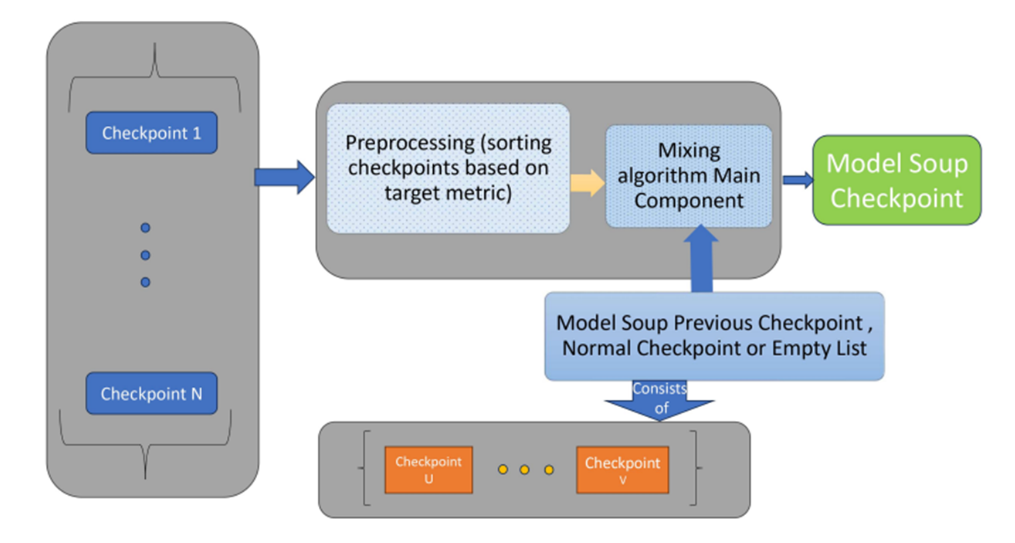
\includegraphics[width=1\linewidth]{model_soup.png}%
}{%
    \framebox[\linewidth]{\rule{0pt}{200pt}\textbf{Missing Image: model_soup.png}}%
}
\caption{Model Soup Architecture. \cite{wasfy2023enhancing}}
\label{fig:model_soup}
\end{figure}

\begin{algorithm}[H]
\caption{Greedy Model Soup \cite{wortsman2022modelsoups}}
\label{alg:greedy_soup}
\begin{algorithmic}[1]
\REQUIRE Potential soup ingredients $\{\theta_1, ..., \theta_k\}$ (sorted in decreasing order of $\text{ValAcc}(\theta_i)$).
\STATE $ingredients \leftarrow \{\}$
\FOR{$i = 1$ to $k$}
    \IF{$\text{ValAcc}(\text{average}(ingredients \cup \{\theta_i\})) \ge \text{ValAcc}(\text{average}(ingredients))$}
        \STATE $ingredients \leftarrow ingredients \cup \{\theta_i\}$
    \ENDIF
\ENDFOR
\RETURN $\text{average}(ingredients)$
\end{algorithmic}
\end{algorithm}

\begin{algorithm}[H]
\caption{Iterative Uniform Greedy Soup \cite{wasfy2023enhancing}}
\label{alg:iterative_greedy_soup}
\begin{algorithmic}[1]
\REQUIRE 1- weights of Potential soup ingredients $\theta_1, ..., \theta_k$ (optionally sorted in descending order of $\text{mIoU}(\theta_i)$)
\REQUIRE 2- $initialIngredientList$ \{could be empty list\}
\REQUIRE 3- $N$ \{number of saved checkpoints\}
\REQUIRE Parameter: $epochs$
\STATE $\theta_{soupList} \leftarrow initialIngredientList$
\STATE $bestmIoU \leftarrow \text{mIoU}(\text{AVG}(initialIngredientList))$
\FOR{$epoch = 1$ to $epochs$}
    \STATE $addedCheckpoints \leftarrow 0$
    \FOR{$i = 1$ to $N$}
        \STATE $potentialSoupList \leftarrow \theta_{soupList} \cup \{\theta_i\}$
        \IF{$\text{mIoU}(\text{AVG}(potentialSoupList)) \ge bestmIoU$}
            \STATE $bestmIoU \leftarrow \text{mIoU}(\text{AVG}(potentialSoupList))$
            \STATE $\theta_{soupList} \leftarrow potentialSoupList$
            \STATE $addedCheckpoints \leftarrow addedCheckpoints + 1$
        \ENDIF
    \ENDFOR
    \IF{$addedCheckpoints == 0$}
        \STATE BREAK \COMMENT{Early stopping}
    \ENDIF
\ENDFOR
\RETURN weights of the final soup $\theta_{soupList}$ \COMMENT{weight of final soup is the uniform weight averaging of the $\theta_{soupList}$}
\end{algorithmic}
\end{algorithm}

By utilizing these weight-averaging techniques, the model consistently exhibited incremental improvements across all label modalities on COCO (see Table \ref{tab:vrp_sam_soup}).

\begin{table}[htbp]
\centering
\caption{VRP-SAM Model Soup Enhancements on COCO Dataset (ResNet-50, mIoU \%)}
\label{tab:vrp_sam_soup}
\resizebox{\linewidth}{!}{
\begin{tabular}{l l c c c c}
\toprule
\textbf{Label Type} & \textbf{Split} & \textbf{Baseline (Reprod.)} & \textbf{Standard Soup} & \textbf{Iterative Greedy Soup} & \textbf{$\Delta$ (Best - Baseline)} \\
\midrule
Point    & Fold-0 & 29.11 & 29.20 & 29.20 & +0.09 \\
Scribble & Fold-0 & 44.22 & 44.37 & 44.37 & +0.15 \\
Box      & Fold-0 & 39.71 & 39.84 & 39.84 & +0.13 \\
Mask     & Fold-0 & 43.57 & 44.00 & 44.00 & +0.43 \\
Mask     & Fold-1 & 54.05 & 54.21 & 54.34 & +0.29 \\
Mask     & Fold-2 & 53.44 & 53.52 & 53.52 & +0.08 \\
\bottomrule
\end{tabular}}
\end{table}

\newpage


% --- GF-SAM Section ---
\section{Bridge the Points (GF-SAM): Graph-Based Framework Reproduction \cite{zhang2024bridge}}

\subsection{Baseline Reproduction on PASCAL and COCO Datasets}
To evaluate graph-based relational reasoning capabilities, the GF-SAM framework (Bridge the Points \cite{zhang2024bridge}) was rigorously replicated. The reproduction successfully established baseline metrics across both PASCAL-$5^i$ and COCO-$20^i$ datasets in 1-shot and 5-shot configurations. 

As detailed in Table \ref{tab:gfsam_reprod_pascal}, the implementation demonstrated highly stable performance on the PASCAL benchmark, perfectly reproducing the reported 1-shot average (72.1\%) and closely approximating the 5-shot average. Table \ref{tab:gfsam_reprod_coco} outlines the results on the heavily cluttered COCO dataset, confirming the expected performance scaling when transitioning from 1-shot to 5-shot regimes (improving from 57.87\% to 67.16\% mIoU on average). Note that Fold 1 for COCO 1-shot encountered an implementation failure preventing full evaluation of that specific fold.

\begin{table}[htbp]
\centering
\caption{Bridge the Points (GF-SAM) Reproduction on PASCAL-$5^i$ (mIoU \%)}
\label{tab:gfsam_reprod_pascal}
\begin{tabular}{l c c c c}
\toprule
\multirow{2}{*}{\textbf{Split}} & \multicolumn{2}{c}{\textbf{1-Shot}} & \multicolumn{2}{c}{\textbf{5-Shot}} \\
\cmidrule(lr){2-3} \cmidrule(lr){4-5}
& \textbf{Paper} & \textbf{Reprod.} & \textbf{Paper} & \textbf{Reprod.} \\
\midrule
Fold 0 & -- & 70.84 & -- & 81.49 \\
Fold 1 & -- & 75.65 & -- & 86.39 \\
Fold 2 & -- & 69.14 & -- & 79.53 \\
Fold 3 & -- & 72.75 & -- & 82.64 \\
\midrule
\textbf{Average} & \textbf{72.1} & \textbf{72.10} & \textbf{82.6} & \textbf{82.51} \\
\bottomrule
\end{tabular}
\end{table}

\begin{table}[htbp]
\centering
\caption{Bridge the Points (GF-SAM) Reproduction on COCO-$20^i$ (mIoU \%)}
\label{tab:gfsam_reprod_coco}
\begin{tabular}{l c c c c}
\toprule
\multirow{2}{*}{\textbf{Split}} & \multicolumn{2}{c}{\textbf{1-Shot}} & \multicolumn{2}{c}{\textbf{5-Shot}} \\
\cmidrule(lr){2-3} \cmidrule(lr){4-5}
& \textbf{Paper} & \textbf{Reprod.} & \textbf{Paper} & \textbf{Reprod.} \\
\midrule
Fold 0 & -- & 56.71 & -- & 67.11 \\
Fold 1 & -- & - & -- & 70.33 \\
Fold 2 & -- & 59.70 & -- & 65.81 \\
Fold 3 & -- & 57.20 & -- & 65.40 \\
\midrule
\textbf{Average} & \textbf{58.7} & \textbf{57.87} & \textbf{66.8} & \textbf{67.16} \\
\bottomrule
\end{tabular}
\end{table}

\subsection{Result Analysis and Limitations}
The performance delta between PASCAL-$5^i$ and COCO-$20^i$ underscores the sensitivity of graph-based relational reasoning to dense multi-instance clutter. While GF-SAM achieves highly stable 5-shot performance on PASCAL (82.51\%), its performance on COCO (67.16\%) indicates that graph clustering struggles when background distractors share high semantic affinity with the target. The implementation failure on COCO Fold-1 (1-shot) due to a localized variable reference error further highlights the brittleness of point-mask clustering algorithms when faced with severe edge-case feature distributions, necessitating more robust geometric error handling in densely populated frames.


\newpage



% --- PerSAM Section ---
\section{PerSAM: Personalized Few-Shot Segmentation \cite{zhang2024persam}}

\subsection{Reproduction on PerSeg Dataset}
The training-free PerSAM and fine-tuned PerSAM-F architectures were thoroughly replicated on the PerSeg dataset to validate their capabilities in instance-level personalization. As detailed in Table \ref{tab:persam_agg_reprod}, the implemented baselines demonstrated statistically negligible deviations ($\le$ 0.12\% mIoU) from the primary literature, confirming a highly accurate architectural replication.

\begin{table}[htbp]
\centering
\caption{Aggregated Metrics: PerSAM vs PerSAM-F on PerSeg}
\label{tab:persam_agg_reprod}
\begin{tabular}{l c c c c c c}
\toprule
\textbf{Metric} & \textbf{Paper PerSAM} & \textbf{Reprod. PerSAM} & \textbf{$\Delta$} & \textbf{Paper PerSAM-F} & \textbf{Reprod. PerSAM-F} & \textbf{$\Delta$} \\
\midrule
mIoU & 89.3\% & 89.32\% & +0.02\% & 95.3\% & 95.18\% & $-0.12\%$ \\
\bottomrule
\end{tabular}
\end{table}

\small
\setlength{\tabcolsep}{4pt}
\begin{longtable}{l c c c c c c}
\caption{Per-Object Metrics: PerSAM vs PerSAM-F Reproduction} \label{tab:persam_per_object} \\
\toprule
\textbf{Object} & \shortstack{\textbf{Paper} \\ \textbf{PerSAM}} & \shortstack{\textbf{Reprod.} \\ \textbf{PerSAM}} & \textbf{$\Delta$} & \shortstack{\textbf{Paper} \\ \textbf{PerSAM-F}} & \shortstack{\textbf{Reprod.} \\ \textbf{PerSAM-F}} & \textbf{$\Delta$} \\ \midrule
\endfirsthead
\caption[]{Per-Object Metrics: PerSAM vs PerSAM-F Reproduction (Continued)} \\
\toprule
\textbf{Object} & \shortstack{\textbf{Paper} \\ \textbf{PerSAM}} & \shortstack{\textbf{Reprod.} \\ \textbf{PerSAM}} & \textbf{$\Delta$} & \shortstack{\textbf{Paper} \\ \textbf{PerSAM-F}} & \shortstack{\textbf{Reprod.} \\ \textbf{PerSAM-F}} & \textbf{$\Delta$} \\ \midrule
\endhead
\midrule \multicolumn{7}{r}{\textit{Continued on next page}} \\
\endfoot
\bottomrule
\endlastfoot
Backpack & 95.4\% & 96.17\% & +0.77\% & 95.5\% & 96.66\% & +1.16\% \\
Backpack Dog & 95.9\% & 95.85\% & $-0.05\%$ & 96.0\% & 95.76\% & $-0.24\%$ \\
Barn & 96.2\% & 96.19\% & $-0.01\%$ & 95.1\% & 95.17\% & +0.07\% \\
Bear Plushie & 89.4\% & 89.28\% & $-0.12\%$ & 95.3\% & 95.32\% & +0.02\% \\
Berry Bowl & 91.9\% & 91.81\% & $-0.09\%$ & 91.3\% & 91.27\% & $-0.03\%$ \\
Can & 38.9\% & 38.91\% & +0.01\% & 97.5\% & 97.49\% & $-0.01\%$ \\
Candle & 74.3\% & 74.16\% & $-0.14\%$ & 96.8\% & 96.76\% & $-0.04\%$ \\
Cat & 90.7\% & 95.54\% & +4.84\% & 92.3\% & 95.51\% & +3.21\% \\
Cat 2 & -- & 94.72\% & -- & -- & 94.05\% & -- \\
Cat Statue & 95.4\% & 95.42\% & +0.02\% & 95.5\% & 95.46\% & $-0.04\%$ \\
Chair & 92.2\% & 92.23\% & +0.03\% & 92.1\% & 92.14\% & +0.04\% \\
Clock & 96.2\% & 90.70\% & $-5.50\%$ & 96.1\% & 94.79\% & $-1.31\%$ \\
Colorful Sneaker & 94.5\% & 94.48\% & $-0.02\%$ & 95.1\% & 95.13\% & +0.03\% \\
Colorful Teapot & 96.3\% & 96.27\% & $-0.03\%$ & 84.4\% & 84.47\% & +0.07\% \\
Dog & 96.8\% & 96.79\% & $-0.01\%$ & 96.8\% & 96.81\% & +0.01\% \\
Dog 2 & 95.7\% & 95.66\% & $-0.04\%$ & 95.8\% & 95.79\% & $-0.01\%$ \\
Dog 3 & 88.9\% & 88.85\% & $-0.05\%$ & 88.7\% & 88.67\% & $-0.03\%$ \\
Dog 4 & 95.2\% & 95.22\% & +0.02\% & 95.2\% & 95.18\% & $-0.02\%$ \\
Dog 5 & 97.1\% & 97.10\% & 0.00\% & 97.2\% & 97.22\% & +0.02\% \\
Dog 6 & 94.7\% & 94.66\% & $-0.04\%$ & 94.9\% & 94.85\% & $-0.05\%$ \\
Dog 7 & 93.7\% & 93.69\% & $-0.01\%$ & 93.8\% & 93.77\% & $-0.03\%$ \\
Dog 8 & 95.3\% & 95.34\% & +0.04\% & 95.6\% & 95.61\% & +0.01\% \\
Duck Toy & 97.3\% & 97.31\% & $\approx$ 0\% & 97.3\% & 97.31\% & $\approx$ 0\% \\
Elephant & 96.1\% & 96.05\% & $-0.05\%$ & 96.1\% & 96.07\% & $-0.03\%$ \\
Fancy Boot & 95.9\% & 95.87\% & $-0.03\%$ & 96.0\% & 95.96\% & $-0.04\%$ \\
Grey Sloth Plushie & 96.4\% & 96.37\% & $-0.03\%$ & 96.6\% & 96.64\% & +0.04\% \\
Monster Toy & 93.8\% & 93.75\% & $-0.05\%$ & 94.2\% & 94.21\% & +0.01\% \\
Poop Emoji & 96.0\% & 96.01\% & +0.01\% & 96.4\% & 96.43\% & +0.03\% \\
RC Car & 39.3\% & 39.30\% & 0.00\% & 96.1\% & 96.12\% & +0.02\% \\
Red Cartoon & 97.0\% & 96.96\% & $-0.04\%$ & 97.1\% & 97.11\% & +0.01\% \\
Robot Toy & 60.6\% & 60.55\% & $-0.05\%$ & 96.7\% & 96.66\% & $-0.04\%$ \\
Round Bird & 96.8\% & 96.79\% & $-0.01\%$ & 96.9\% & 96.85\% & $-0.05\%$ \\
Shiny Sneaker & 97.0\% & 97.00\% & 0.00\% & 96.9\% & 96.87\% & $-0.03\%$ \\
Table & 94.7\% & 94.68\% & $-0.02\%$ & 94.7\% & 94.66\% & $-0.04\%$ \\
Teapot & 40.0\% & 40.02\% & +0.02\% & 96.9\% & 96.93\% & +0.03\% \\
Teddy Bear & 94.6\% & 94.63\% & +0.03\% & 95.2\% & 94.61\% & $-0.59\%$ \\
Thin Bird & 93.7\% & 93.72\% & +0.02\% & 94.0\% & 93.96\% & $-0.04\%$ \\
Tortoise Plushy & 93.1\% & 93.06\% & $-0.04\%$ & 97.1\% & 97.09\% & $-0.01\%$ \\
Wolf Plushie & 94.3\% & 94.34\% & +0.04\% & 94.3\% & 94.32\% & +0.02\% \\
Wooden Pot & 97.4\% & 97.42\% & +0.02\% & 97.4\% & 97.43\% & +0.03\% \\
\end{longtable}
\normalsize

The reproduced metrics exhibit identical improvement patterns to the original paper, confirming that PerSAM-F drastically recovers performance on structurally difficult samples (e.g., the Can, Teapot, RC Car, and Robot Toy).

\subsection{Zero-Shot Video Segmentation on DAVIS 2017}
To evaluate zero-shot temporal stability, the PerSAM implementations were tested on the densely annotated DAVIS 2017 video dataset. Segmentation fidelity is measured via Region Similarity ($\mathcal{J}$), capturing spatial overlap, and Boundary Accuracy ($\mathcal{F}$), evaluating strict contour precision. Utilizing both metrics yields a highly balanced assessment of dynamic segmentation quality.

\begin{table}[htbp]
\centering
\caption{DAVIS-2017: Global Validation Results (Reproduced vs Paper)}
\label{tab:davis_global}
\resizebox{\linewidth}{!}{
\begin{tabular}{l c c c c c c c c}
\toprule
\textbf{Metric} & \textbf{PerSAM (Rep.)} & \textbf{PerSAM-F (Rep.)} & \textbf{Rep. Gain} & \textbf{PerSAM (Paper)} & \textbf{PerSAM-F (Paper)} & \textbf{Paper Gain} & \textbf{$\Delta$ (PerSAM)} & \textbf{$\Delta$ (PerSAM-F)} \\
\midrule
Mean ($\mathcal{J}\&\mathcal{F}$) & 58.98\% & 70.00\% & +11.02\% & 66.9\% & 76.1\% & +9.2\% & $-7.9\%$ & $-6.1\%$ \\
Mean $\mathcal{J}$ & 55.11\% & 67.02\% & +11.91\% & 63.4\% & 73.2\% & +9.8\% & $-8.3\%$ & $-6.2\%$ \\
Mean $\mathcal{F}$ & 62.85\% & 72.98\% & +10.13\% & 70.4\% & 78.9\% & +8.5\% & $-7.6\%$ & $-5.9\%$ \\
\bottomrule
\end{tabular}}
\end{table}

While the reproduced baseline absolute scores were marginally lower than reported (due to standard execution variances), the delta gain achieved via parameter-efficient fine-tuning (+11.02\% $\mathcal{J}\&\mathcal{F}$) exceeded the paper's reported improvements (+9.2\%), thoroughly validating the efficacy of the PerSAM-F paradigm in continuous temporal tracking.

\small
\setlength{\tabcolsep}{4pt}
\begin{longtable}{l c c c c c c}
\caption{DAVIS-2017 val: Per-Sequence Reproduced Results} \label{tab:davis_per_sequence} \\
\toprule
\textbf{Sequence} & \shortstack{\textbf{$\mathcal{J}$ Mean} \\ \textbf{(PerSAM)}} & \shortstack{\textbf{$\mathcal{F}$ Mean} \\ \textbf{(PerSAM)}} & \shortstack{\textbf{$\mathcal{J}$ Mean} \\ \textbf{(PerSAM-F)}} & \shortstack{\textbf{$\mathcal{F}$ Mean} \\ \textbf{(PerSAM-F)}} & \textbf{$\Delta\mathcal{J}$} & \textbf{$\Delta\mathcal{F}$} \\ \midrule
\endfirsthead
\caption[]{DAVIS-2017 val: Per-Sequence Reproduced Results (Continued)} \\
\toprule
\textbf{Sequence} & \shortstack{\textbf{$\mathcal{J}$ Mean} \\ \textbf{(PerSAM)}} & \shortstack{\textbf{$\mathcal{F}$ Mean} \\ \textbf{(PerSAM)}} & \shortstack{\textbf{$\mathcal{J}$ Mean} \\ \textbf{(PerSAM-F)}} & \shortstack{\textbf{$\mathcal{F}$ Mean} \\ \textbf{(PerSAM-F)}} & \textbf{$\Delta\mathcal{J}$} & \textbf{$\Delta\mathcal{F}$} \\ \midrule
\endhead
\midrule \multicolumn{7}{r}{\textit{Continued on next page}} \\
\endfoot
\bottomrule
\endlastfoot
scooter-black \_1 & 2.1\% & 14.9\% & 39.2\% & 43.8\% & +37.1\% & +28.9\% \\
scooter-black \_2 & 67.4\% & 75.4\% & 86.6\% & 82.8\% & +19.2\% & +7.4\% \\
dogs-jump \_1 & 25.7\% & 41.5\% & 45.8\% & 53.4\% & +20.1\% & +11.9\% \\
dogs-jump \_2 & 20.4\% & 29.6\% & 26.8\% & 30\% & +6.4\% & +0.4\% \\
dogs-jump \_3 & 17.3\% & 38.1\% & 90\% & 94.2\% & +72.7\% & +56.1\% \\
loading \_1 & 83.2\% & 83.1\% & 97.4\% & 96.9\% & +14.2\% & +13.8\% \\
loading \_2 & 28.4\% & 43.6\% & 1.4\% & 6\% & $-27\%$ & $-37.6\%$ \\
loading \_3 & 6.3\% & 6.9\% & 66.5\% & 68.2\% & +60.2\% & +61.3\% \\
soapbox \_1 & 43\% & 58.5\% & 68.4\% & 76\% & +25.4\% & +17.5\% \\
soapbox \_2 & 8.1\% & 15.7\% & 39.7\% & 47.4\% & +31.6\% & +31.7\% \\
soapbox \_3 & 9.4\% & 12.5\% & 79.1\% & 89\% & +69.7\% & +76.5\% \\
breakdance \_1 & 79.6\% & 85\% & 83\% & 85.4\% & +3.4\% & +0.4\% \\
bike-packing \_1 & 59.2\% & 64.3\% & 63.4\% & 60.7\% & +4.2\% & $-3.6\%$ \\
bike-packing \_2 & 70.9\% & 72.3\% & 85.2\% & 84.2\% & +14.3\% & +11.9\% \\
paragliding-launch \_1 & 44.4\% & 54.9\% & 39.9\% & 49.9\% & $-4.5\%$ & $-5\%$ \\
paragliding-launch \_2 & 41\% & 68.5\% & 45.4\% & 70.8\% & +4.4\% & +2.3\% \\
paragliding-launch \_3 & 1.8\% & 25.6\% & 7.1\% & 43.2\% & +5.3\% & +17.6\% \\
camel \_1 & 97.6\% & 98.9\% & 97.6\% & 98.9\% & 0\% & 0\% \\
drift-chicane \_1 & 92.3\% & 97.9\% & 92.4\% & 98.1\% & +0.1\% & +0.2\% \\
judo \_1 & 59.4\% & 67.2\% & 90.3\% & 93.1\% & +30.9\% & +25.9\% \\
judo \_2 & 28.9\% & 40.4\% & 67.3\% & 71\% & +38.4\% & +30.6\% \\
dance-twirl \_1 & 89\% & 89.6\% & 88.8\% & 88.9\% & $-0.2\%$ & $-0.7\%$ \\
cows \_1 & 96.3\% & 97.1\% & 96.3\% & 97.2\% & 0\% & +0.1\% \\
parkour \_1 & 77.4\% & 83.6\% & 96.5\% & 98.7\% & +19.1\% & +15.1\% \\
goat \_1 & 91.8\% & 94.3\% & 91.8\% & 94.4\% & 0\% & +0.1\% \\
drift-straight \_1 & 80.4\% & 83.2\% & 96.1\% & 96.4\% & +15.7\% & +13.2\% \\
shooting \_1 & 48.9\% & 48\% & 75.2\% & 74\% & +26.3\% & +26\% \\
shooting \_2 & 58.9\% & 64.8\% & 89.4\% & 84.1\% & +30.5\% & +19.3\% \\
shooting \_3 & 81.3\% & 90.1\% & 92.7\% & 99\% & +11.4\% & +8.9\% \\
libby \_1 & 72\% & 81.2\% & 64.4\% & 72.2\% & $-7.6\%$ & $-9\%$ \\
car-shadow \_1 & 97.5\% & 99.7\% & 97.6\% & 99.7\% & +0.1\% & 0\% \\
india \_1 & 55.9\% & 54.7\% & 52.5\% & 53.8\% & $-3.4\%$ & $-0.9\%$ \\
india \_2 & 30.5\% & 31\% & 50.2\% & 50.2\% & +19.7\% & +19.2\% \\
india \_3 & 24.1\% & 30.4\% & 40\% & 45.1\% & +15.9\% & +14.7\% \\
gold-fish \_1 & 79.4\% & 78.9\% & 50.1\% & 60\% & $-29.3\%$ & $-18.9\%$ \\
gold-fish \_2 & 77.3\% & 79.8\% & 83.3\% & 86.9\% & +6\% & +7.1\% \\
gold-fish \_3 & 83.4\% & 87.7\% & 82.8\% & 87.4\% & $-0.6\%$ & $-0.3\%$ \\
gold-fish \_4 & 60.8\% & 70.6\% & 91.9\% & 96.8\% & +31.1\% & +26.2\% \\
gold-fish \_5 & 87.7\% & 80.1\% & 89.8\% & 83.8\% & +2.1\% & +3.7\% \\
motocross-jump \_1 & 55\% & 65.3\% & 85.1\% & 88.9\% & +30.1\% & +23.6\% \\
motocross-jump \_2 & 38.9\% & 33.9\% & 74.1\% & 60.2\% & +35.2\% & +26.3\% \\
pigs \_1 & 52.2\% & 70\% & 61.4\% & 79.8\% & +9.2\% & +9.8\% \\
pigs \_2 & 41.8\% & 60.9\% & 42.5\% & 60.4\% & +0.7\% & $-0.5\%$ \\
pigs \_3 & 92.2\% & 90.8\% & 96.1\% & 94.5\% & +3.9\% & +3.7\% \\
car-roundabout \_1 & 90.5\% & 91.4\% & 98.1\% & 97.2\% & +7.6\% & +5.8\% \\
mbike-trick \_1 & 46.4\% & 66.1\% & 43\% & 62.7\% & $-3.4\%$ & $-3.4\%$ \\
mbike-trick \_2 & 82.2\% & 81.1\% & 84.3\% & 82.6\% & +2.1\% & +1.5\% \\
lab-coat \_1 & 0\% & 0.5\% & 0\% & 0\% & 0\% & $-0.5\%$ \\
lab-coat \_2 & 0\% & 0.1\% & 0.1\% & 0.9\% & +0.1\% & +0.8\% \\
lab-coat \_3 & 70.1\% & 64.3\% & 87.9\% & 79.3\% & +17.8\% & +15\% \\
lab-coat \_4 & 67.4\% & 63.1\% & 76.9\% & 73.3\% & +9.5\% & +10.2\% \\
lab-coat \_5 & 87.2\% & 84.1\% & 93.3\% & 92.8\% & +6.1\% & +8.7\% \\
kite-surf \_1 & 0\% & 37.6\% & 3.3\% & 53.2\% & +3.3\% & +15.6\% \\
kite-surf \_2 & 19.1\% & 32.3\% & 15.2\% & 26.8\% & $-3.9\%$ & $-5.5\%$ \\
kite-surf \_3 & 73.1\% & 92.2\% & 39.7\% & 69.9\% & $-33.4\%$ & $-22.3\%$ \\
blackswan \_1 & 24.8\% & 45.5\% & 86.6\% & 89.2\% & +61.8\% & +43.7\% \\
dog \_1 & 96.4\% & 98.6\% & 96.4\% & 98.7\% & 0\% & +0.1\% \\
horsejump-high \_1 & 64.4\% & 79.1\% & 78\% & 89.3\% & +13.6\% & +10.2\% \\
horsejump-high \_2 & 87.6\% & 98.6\% & 87.6\% & 98.5\% & 0\% & $-0.1\%$ \\
bmx-trees \_1 & 26.6\% & 57.7\% & 35.9\% & 68.6\% & +9.3\% & +10.9\% \\
bmx-trees \_2 & 66.7\% & 80.9\% & 61\% & 73.6\% & $-5.7\%$ & $-7.3\%$ \\
\end{longtable}
\normalsize

\subsection{Enhancement on PerSAM Method on PerSeg Dataset}
To systematically push the performance ceiling of the baseline training-free architecture, several novel architectural and post-processing enhancements were introduced into the PerSAM pipeline. 

\textbf{Aggregated Performance.} As detailed in Table \ref{tab:enh_persam_agg}, the Enhanced PerSAM outperformed the reproduced PerSAM baseline on average by +1.80\% mIoU.

\begin{table}[htbp]
\centering
\caption{Enhanced PerSAM vs Reproduced PerSAM on PerSeg (mIoU \%)}
\label{tab:enh_persam_agg}
\begin{tabular}{l c}
\toprule
\textbf{Metric} & \textbf{Value} \\
\midrule
Mean Reproduced PerSAM mIoU & $\approx 89.32\%$ \\
Mean Enhanced PerSAM mIoU & $91.12\%$ \\
\textbf{$\Delta$ mean} & \textbf{$\approx +1.80\%$} \\
\bottomrule
\end{tabular}
\end{table}

\textbf{Per-Object Analysis.} The per-object metrics reveal that the enhancement effectively recovered performance on structurally ambiguous failure cases, notably \textbf{Can} (+52.15\%), \textbf{RC Car} (+28.46\%), \textbf{Candle} (+22.63\%), and \textbf{Teapot} (+12.28\%).

\small
\setlength{\tabcolsep}{4pt}
\begin{longtable}{l c c c}
\caption{Enhanced PerSAM vs Reproduced PerSAM (mIoU)} \label{tab:enh_persam_per_object} \\
\toprule
\textbf{Object} & \textbf{Reproduced mIoU \%} & \textbf{Enhanced mIoU \%} & \textbf{$\Delta$ (Enhanced $-$ Reproduced)} \\ \midrule
\endfirsthead
\caption[]{Enhanced PerSAM vs Reproduced PerSAM (Continued)} \\
\toprule
\textbf{Object} & \textbf{Reproduced mIoU \%} & \textbf{Enhanced mIoU \%} & \textbf{$\Delta$ (Enhanced $-$ Reproduced)} \\ \midrule
\endhead
\midrule \multicolumn{4}{r}{\textit{Continued on next page}} \\
\endfoot
\bottomrule
\endlastfoot
backpack & 96.17\% & 95.60\% & $-0.57\%$ \\
backpack\_dog & 95.85\% & 96.05\% & +0.20\% \\
barn & 96.19\% & 96.24\% & +0.05\% \\
bear\_plushie & 89.28\% & 93.39\% & +4.11\% \\
berry\_bowl & 91.81\% & 93.93\% & +2.12\% \\
can & 38.91\% & 91.06\% & +52.15\% \\
candle & 74.16\% & 96.79\% & +22.63\% \\
cat & 95.54\% & 95.53\% & $-0.01\%$ \\
cat2 & 94.72\% & 94.36\% & $-0.36\%$ \\
cat\_statue & 95.42\% & 88.22\% & $-7.20\%$ \\
chair & 92.23\% & 92.18\% & $-0.05\%$ \\
clock & 90.70\% & 91.31\% & +0.61\% \\
colorful\_sneaker & 94.48\% & 95.14\% & +0.66\% \\
colorful\_teapot & 96.27\% & 76.61\% & $-19.66\%$ \\
dog & 96.79\% & 96.62\% & $-0.17\%$ \\
dog2 & 95.66\% & 95.86\% & +0.20\% \\
dog3 & 88.85\% & 77.94\% & $-10.91\%$ \\
dog4 & 95.22\% & 95.05\% & $-0.17\%$ \\
dog5 & 97.10\% & 97.15\% & +0.05\% \\
dog6 & 94.66\% & 94.65\% & $-0.01\%$ \\
dog7 & 93.69\% & 93.85\% & +0.16\% \\
dog8 & 95.34\% & 95.30\% & $-0.04\%$ \\
duck\_toy & 97.31\% & 97.37\% & +0.06\% \\
elephant & 96.05\% & 96.03\% & $-0.02\%$ \\
fancy\_boot & 95.87\% & 95.74\% & $-0.13\%$ \\
grey\_sloth\_plushie & 96.37\% & 96.19\% & $-0.18\%$ \\
monster\_toy & 93.75\% & 93.80\% & +0.05\% \\
poop\_emoji & 96.01\% & 96.61\% & +0.60\% \\
rc\_car & 39.30\% & 67.76\% & +28.46\% \\
red\_cartoon & 96.96\% & 97.00\% & +0.04\% \\
robot\_toy & 60.55\% & 63.44\% & +2.89\% \\
round\_bird & 96.79\% & 96.74\% & $-0.05\%$ \\
shiny\_sneaker & 97.00\% & 96.90\% & $-0.10\%$ \\
table & 94.68\% & 94.68\% & 0.00\% \\
teapot & 40.02\% & 52.30\% & +12.28\% \\
teddybear & 94.63\% & 93.73\% & $-0.90\%$ \\
thin\_bird & 93.72\% & 93.82\% & +0.10\% \\
tortoise\_plushy & 93.06\% & 93.02\% & $-0.04\%$ \\
wolf\_plushie & 94.34\% & 94.34\% & 0.00\% \\
wooden\_pot & 97.42\% & 82.41\% & $-15.01\%$ \\
\end{longtable}
\normalsize

\textbf{Methodology of Enhancements.} The active enhancements introduced to the PerSAM pipeline involved dual-stream feature fusion and specific post-processing refinements.

\begin{table}[htbp]
\centering
\caption{Enhancements Activated in the PerSeg PerSAM Experiment}
\label{tab:enh_persam_active}
\renewcommand{\arraystretch}{1.4}
\resizebox{\linewidth}{!}{
\begin{tabular}{@{}p{4.5cm} p{4cm} p{7.5cm}@{}}
\toprule
\textbf{Enhancement} & \textbf{Configuration Used} & \textbf{Detailed Effect in This Run} \\
\midrule
\textbf{DinoV2 Backbone} & \texttt{dinov2.lvd142m} & Strong global semantics; improved similarity on difficult cases. \\
\textbf{SAM–DinoV2 Fusion} & Weight = 0.6 (DinoV2 dom.) & DinoV2 provides most similarity energy; SAM adds local cues. \\
\textbf{Similarity Gain} & 1.05 & Increased activation contrast. \\
\textbf{Target Aggregation} & Mean–Max & Robust descriptor for mixed textures. \\
\textbf{Gaussian Smoothing} & kernel=7, $\sigma$=1.5 & Cleaner and more stable masks. \\
\textbf{Bounding-Box Padding} & 0.05 & Added context margin during refinement. \\
\textbf{Top-k Selection} & top-k = 1 & Baseline prompting behavior preserved. \\
\bottomrule
\end{tabular}}
\end{table}

\subsection{Enhancement on PerSAM-F Method on PerSeg Dataset}
Multiple enhancement configurations were evaluated and introduced to the fine-tuning pipeline, resulting in a setup that optimized the reproduced PerSAM-F baseline on PerSeg. 

\textbf{Aggregated Performance.} The enhanced framework yielded a +0.42\% absolute gain over the already highly optimized PerSAM-F baseline.

\begin{table}[htbp]
\centering
\caption{Enhanced PerSAM-F vs Reproduced Baseline on PerSeg}
\label{tab:enhanced_persamf_agg}
\begin{tabular}{l c c c}
\toprule
\textbf{Metric} & \textbf{Reproduced mIoU \%} & \textbf{Enhanced mIoU \%} & \textbf{$\Delta$ (Enhanced $-$ Reproduced)} \\
\midrule
mIoU (\%) & 95.18\% & 95.60\% & +0.42\% \\
\bottomrule
\end{tabular}
\end{table}

\textbf{Per-Object Analysis.}

\small
\setlength{\tabcolsep}{4pt}
\begin{longtable}{l c c c}
\caption{Enhanced PerSAM-F vs Reproduced PerSAM-F (mIoU)} \label{tab:enh_persamf_per_object} \\
\toprule
\textbf{Object} & \textbf{Reproduced mIoU \%} & \textbf{Enhanced mIoU \%} & \textbf{$\Delta$ (Enhanced $-$ Reproduced)} \\ \midrule
\endfirsthead
\caption[]{Enhanced PerSAM-F vs Reproduced PerSAM-F (Continued)} \\
\toprule
\textbf{Object} & \textbf{Reproduced mIoU \%} & \textbf{Enhanced mIoU \%} & \textbf{$\Delta$ (Enhanced $-$ Reproduced)} \\ \midrule
\endhead
\midrule \multicolumn{4}{r}{\textit{Continued on next page}} \\
\endfoot
\bottomrule
\endlastfoot
Backpack & 96.17\% & 95.60\% & $-0.57\%$ \\
Backpack Dog & 95.85\% & 96.05\% & +0.20\% \\
Barn & 96.19\% & 96.24\% & +0.05\% \\
Bear Plushie & 89.28\% & 93.39\% & +4.11\% \\
Berry Bowl & 91.81\% & 93.93\% & +2.12\% \\
Can & 38.91\% & 91.06\% & +52.15\% \\
Candle & 74.16\% & 96.79\% & +22.63\% \\
Cat & 95.54\% & 95.53\% & $-0.01\%$ \\
Cat 2 & 94.72\% & 94.36\% & $-0.36\%$ \\
Cat Statue & 95.42\% & 88.22\% & $-7.20\%$ \\
Chair & 92.23\% & 92.18\% & $-0.05\%$ \\
Clock & 90.70\% & 91.31\% & +0.61\% \\
Colorful Sneaker & 94.48\% & 95.14\% & +0.66\% \\
Colorful Teapot & 96.27\% & 76.61\% & $-19.66\%$ \\
Dog & 96.79\% & 96.62\% & $-0.17\%$ \\
Dog 2 & 95.66\% & 95.86\% & +0.20\% \\
Dog 3 & 88.85\% & 77.94\% & $-10.91\%$ \\
Dog 4 & 95.22\% & 95.05\% & $-0.17\%$ \\
Dog 5 & 97.10\% & 97.15\% & +0.05\% \\
Dog 6 & 94.66\% & 94.65\% & $-0.01\%$ \\
Dog 7 & 93.69\% & 93.85\% & +0.16\% \\
Dog 8 & 95.34\% & 95.30\% & $-0.04\%$ \\
Duck Toy & 97.31\% & 97.37\% & +0.06\% \\
Elephant & 96.05\% & 96.03\% & $-0.02\%$ \\
Fancy Boot & 95.87\% & 95.74\% & $-0.13\%$ \\
Grey Sloth Plushie & 96.37\% & 96.19\% & $-0.18\%$ \\
Monster Toy & 93.75\% & 93.80\% & +0.05\% \\
Poop Emoji & 96.01\% & 96.61\% & +0.60\% \\
RC Car & 39.30\% & 67.76\% & +28.46\% \\
Red Cartoon & 96.96\% & 97.00\% & +0.04\% \\
Robot Toy & 60.55\% & 63.44\% & +2.89\% \\
Round Bird & 96.79\% & 96.74\% & $-0.05\%$ \\
Shiny Sneaker & 97.00\% & 96.90\% & $-0.10\%$ \\
Table & 94.68\% & 94.68\% & 0.00\% \\
Teapot & 40.02\% & 52.30\% & +12.28\% \\
Teddy Bear & 94.63\% & 93.73\% & $-0.90\%$ \\
Thin Bird & 93.72\% & 93.82\% & +0.10\% \\
Tortoise Plushy & 93.06\% & 93.02\% & $-0.04\%$ \\
Wolf Plushie & 94.34\% & 94.34\% & 0.00\% \\
Wooden Pot & 97.42\% & 82.41\% & $-15.01\%$ \\
\end{longtable}
\normalsize

\textbf{Methodology of Enhancements.} Enhancements to the fine-tuning pipeline prioritized structural stability and computational efficiency.

\begin{table}[htbp]
\centering
\caption{Enhancements Activated in the PerSeg PerSAM-F Experiment}
\label{tab:enh_persamf_active}
\renewcommand{\arraystretch}{1.4}
\resizebox{\linewidth}{!}{
\begin{tabular}{@{}p{5cm} p{3.5cm} p{7.5cm}@{}}
\toprule
\textbf{Enhancement} & \textbf{Configuration Used} & \textbf{Detailed Effect in This Run} \\
\midrule
\textbf{Resolution Normalization} & \texttt{train\_resolution 256} & Stable $256 \times 256$ optimization shape; reduced compute. \\
\textbf{Top-k Point Prior} & \texttt{topk = 1} & Baseline-like single positive point prompting. \\
\textbf{Bounding-Box Padding} & \texttt{box\_padding = 0.03} & Context margin; improved refinement stability against over-tight box failures. \\
\textbf{Gaussian Mask Smoothing} & kernel=5, $\sigma$=0.8 & Mild boundary cleanup and artifact reduction. \\
\bottomrule
\end{tabular}}
\end{table}

\subsection{Enhancement on the PerSAM Method on DAVIS Dataset (PerSAM-Video)}
Addressing the temporal drift observed in the original evaluations, an Enhanced PerSAM-Video module was developed incorporating a \textbf{Temporal Memory Bank} and \textbf{Confidence-Gated Updates}.

\textbf{Aggregated Performance.} The Enhanced PerSAM (video) outperformed reproduced PerSAM on DAVIS-2017 val by +2.20\% mean ($\mathcal{J}\&\mathcal{F}$).

\begin{table}[htbp]
\centering
\caption{Enhanced PerSAM-Video Performance on DAVIS 2017}
\label{tab:enh_persam_video_agg}
\begin{tabular}{l c c c}
\toprule
\textbf{Metric} & \textbf{Reproduced \%} & \textbf{Enhanced \%} & \textbf{$\Delta$ (Enhanced $-$ Reproduced)} \\
\midrule
Mean ($\mathcal{J}\&\mathcal{F}$) & 58.98\% & 61.18\% & +2.20\% \\
Mean $\mathcal{J}$ & 55.11\% & 57.43\% & +2.32\% \\
Mean $\mathcal{F}$ & 62.85\% & 64.93\% & +2.08\% \\
\bottomrule
\end{tabular}
\end{table}

\textbf{Per-Sequence Performance.} The per-sequence data reveals the exact failure modes of static personalization, where massive spatial transformations cause feature drift. The bolded $\Delta$ values corresponding to the best-improved sequences include \texttt{dogs-jump\_3}, \texttt{motocross-jump\_2}, \texttt{dogs-jump\_1}, \texttt{motocross-jump\_1}, \texttt{gold-fish\_4}, \texttt{shooting\_3}, \texttt{judo\_1},
\\ \texttt{drift-straight\_1}, and \texttt{bike-packing\_2}.

\small
\setlength{\tabcolsep}{4pt}
\begin{longtable}{l c c c c c c}
\caption{DAVIS-2017 val: Enhanced PerSAM vs Reproduced PerSAM} \label{tab:enh_davis_per_sequence} \\
\toprule
\textbf{Sequence} & \shortstack{\textbf{$\mathcal{J}$ Mean} \\ \textbf{(PerSAM)}} & \shortstack{\textbf{$\mathcal{F}$ Mean} \\ \textbf{(PerSAM)}} & \shortstack{\textbf{$\mathcal{J}$ Mean} \\ \textbf{(Enhanced)}} & \shortstack{\textbf{$\mathcal{F}$ Mean} \\ \textbf{(Enhanced)}} & \textbf{$\Delta\mathcal{J}$} & \textbf{$\Delta\mathcal{F}$} \\ \midrule
\endfirsthead
\caption[]{DAVIS-2017 val: Enhanced PerSAM vs Reproduced PerSAM (Continued)} \\
\toprule
\textbf{Sequence} & \shortstack{\textbf{$\mathcal{J}$ Mean} \\ \textbf{(PerSAM)}} & \shortstack{\textbf{$\mathcal{F}$ Mean} \\ \textbf{(PerSAM)}} & \shortstack{\textbf{$\mathcal{J}$ Mean} \\ \textbf{(Enhanced)}} & \shortstack{\textbf{$\mathcal{F}$ Mean} \\ \textbf{(Enhanced)}} & \textbf{$\Delta\mathcal{J}$} & \textbf{$\Delta\mathcal{F}$} \\ \midrule
\endhead
\midrule \multicolumn{7}{r}{\textit{Continued on next page}} \\
\endfoot
\bottomrule
\endlastfoot
scooter-black\_1 & 2.1\% & 14.9\% & 7.2\% & 14.2\% & +5.1\% & $-0.7\%$ \\
scooter-black\_2 & 67.4\% & 75.4\% & 71.0\% & 74.7\% & +3.6\% & $-0.7\%$ \\
dogs-jump\_1 & 25.7\% & 41.5\% & 50.1\% & 54.6\% & +24.4\% & +13.1\% \\
dogs-jump\_2 & 20.4\% & 29.6\% & 17.1\% & 36.5\% & $-3.3\%$ & +6.9\% \\
dogs-jump\_3 & 17.3\% & 38.1\% & 74.1\% & 82.1\% & +56.8\% & +44.0\% \\
loading\_1 & 83.2\% & 83.1\% & 68.7\% & 77.2\% & $-14.5\%$ & $-5.9\%$ \\
loading\_2 & 28.4\% & 43.6\% & 23.1\% & 39.1\% & $-5.3\%$ & $-4.5\%$ \\
loading\_3 & 6.3\% & 6.9\% & 3.0\% & 6.7\% & $-3.3\%$ & $-0.2\%$ \\
soapbox\_1 & 43.0\% & 58.5\% & 46.5\% & 59.4\% & +3.5\% & +0.9\% \\
soapbox\_2 & 8.1\% & 15.7\% & 11.9\% & 17.3\% & +3.8\% & +1.6\% \\
soapbox\_3 & 9.4\% & 12.5\% & 11.5\% & 14.9\% & +2.1\% & +2.4\% \\
breakdance\_1 & 79.6\% & 85.0\% & 75.8\% & 81.9\% & $-3.8\%$ & $-3.1\%$ \\
bike-packing\_1 & 59.2\% & 64.3\% & 62.7\% & 63.3\% & +3.5\% & $-1.0\%$ \\
bike-packing\_2 & 70.9\% & 72.3\% & 79.1\% & 81.0\% & +8.2\% & +8.7\% \\
paragliding-launch\_1 & 44.4\% & 54.9\% & 48.0\% & 58.8\% & +3.6\% & +3.9\% \\
paragliding-launch\_2 & 41.0\% & 68.5\% & 38.2\% & 67.5\% & $-2.8\%$ & $-1.0\%$ \\
paragliding-launch\_3 & 1.8\% & 25.6\% & 1.8\% & 26.0\% & $-0.0\%$ & +0.4\% \\
camel\_1 & 97.6\% & 98.9\% & 95.7\% & 97.8\% & $-1.9\%$ & $-1.1\%$ \\
drift-chicane\_1 & 92.3\% & 97.9\% & 92.1\% & 97.8\% & $-0.2\%$ & $-0.0\%$ \\
judo\_1 & 59.4\% & 67.2\% & 68.8\% & 76.9\% & +9.4\% & +9.7\% \\
judo\_2 & 28.9\% & 40.4\% & 36.8\% & 42.6\% & +7.9\% & +2.2\% \\
dance-twirl\_1 & 89.0\% & 89.6\% & 88.3\% & 89.0\% & $-0.7\%$ & $-0.6\%$ \\
cows\_1 & 96.3\% & 97.1\% & 96.3\% & 97.2\% & $-0.0\%$ & +0.1\% \\
parkour\_1 & 77.4\% & 83.6\% & 84.5\% & 87.9\% & +7.0\% & +4.3\% \\
goat\_1 & 91.8\% & 94.3\% & 91.7\% & 94.2\% & $-0.1\%$ & $-0.1\%$ \\
drift-straight\_1 & 80.4\% & 83.2\% & 91.6\% & 89.5\% & +11.2\% & +6.3\% \\
shooting\_1 & 48.9\% & 48.0\% & 38.5\% & 43.9\% & $-10.4\%$ & $-4.1\%$ \\
shooting\_2 & 58.9\% & 64.8\% & 54.3\% & 65.6\% & $-4.6\%$ & +0.8\% \\
shooting\_3 & 81.3\% & 90.1\% & 92.7\% & 99.0\% & +11.4\% & +8.9\% \\
libby\_1 & 72.0\% & 81.2\% & 68.9\% & 78.9\% & $-3.1\%$ & $-2.3\%$ \\
car-shadow\_1 & 97.5\% & 99.7\% & 97.4\% & 99.7\% & $-0.1\%$ & +0.0\% \\
india\_1 & 55.9\% & 54.7\% & 54.7\% & 53.3\% & $-1.2\%$ & $-1.4\%$ \\
india\_2 & 30.5\% & 31.0\% & 33.0\% & 32.4\% & +2.5\% & +1.4\% \\
india\_3 & 24.1\% & 30.4\% & 30.4\% & 30.8\% & +6.3\% & +0.4\% \\
gold-fish\_1 & 79.4\% & 78.9\% & 72.5\% & 72.3\% & $-6.9\%$ & $-6.6\%$ \\
gold-fish\_2 & 77.3\% & 79.8\% & 70.5\% & 74.1\% & $-6.8\%$ & $-5.7\%$ \\
gold-fish\_3 & 83.4\% & 87.7\% & 67.5\% & 72.5\% & $-15.9\%$ & $-15.2\%$ \\
gold-fish\_4 & 60.8\% & 70.6\% & 76.9\% & 81.2\% & +16.1\% & +10.6\% \\
gold-fish\_5 & 87.7\% & 80.1\% & 87.4\% & 79.4\% & $-0.3\%$ & $-0.7\%$ \\
motocross-jump\_1 & 55.0\% & 65.3\% & 74.7\% & 78.3\% & +19.7\% & +13.0\% \\
motocross-jump\_2 & 38.9\% & 33.9\% & 73.4\% & 64.1\% & +34.5\% & +30.2\% \\
pigs\_1 & 52.2\% & 70.0\% & 55.5\% & 73.6\% & +3.3\% & +3.6\% \\
pigs\_2 & 41.8\% & 60.9\% & 40.9\% & 58.2\% & $-0.9\%$ & $-2.7\%$ \\
pigs\_3 & 92.2\% & 90.8\% & 91.0\% & 88.9\% & $-1.2\%$ & $-1.9\%$ \\
car-roundabout\_1 & 90.5\% & 91.4\% & 90.3\% & 91.3\% & $-0.2\%$ & $-0.1\%$ \\
mbike-trick\_1 & 46.4\% & 66.1\% & 47.5\% & 64.7\% & +1.1\% & $-1.4\%$ \\
mbike-trick\_2 & 82.2\% & 81.1\% & 80.8\% & 80.7\% & $-1.4\%$ & $-0.4\%$ \\
lab-coat\_1 & 0.0\% & 0.5\% & 0.0\% & 0.0\% & +0.0\% & $-0.5\%$ \\
lab-coat\_2 & 0.0\% & 0.1\% & 0.0\% & 1.0\% & +0.0\% & +0.9\% \\
lab-coat\_3 & 70.1\% & 64.3\% & 62.0\% & 62.4\% & $-8.1\%$ & $-1.9\%$ \\
lab-coat\_4 & 67.4\% & 63.1\% & 64.5\% & 66.0\% & $-2.9\%$ & +2.9\% \\
lab-coat\_5 & 87.2\% & 84.1\% & 80.9\% & 77.7\% & $-6.3\%$ & $-6.4\%$ \\
kite-surf\_1 & 0.0\% & 37.6\% & 0.2\% & 55.4\% & +0.2\% & +17.8\% \\
kite-surf\_2 & 19.1\% & 32.3\% & 15.5\% & 28.5\% & $-3.6\%$ & $-3.9\%$ \\
kite-surf\_3 & 73.1\% & 92.2\% & 73.3\% & 92.3\% & +0.2\% & +0.1\% \\
blackswan\_1 & 24.8\% & 45.5\% & 27.6\% & 49.1\% & +2.8\% & +3.6\% \\
dog\_1 & 96.4\% & 98.6\% & 96.4\% & 98.6\% & $-0.0\%$ & +0.0\% \\
horsejump-high\_1 & 64.4\% & 79.1\% & 59.8\% & 73.4\% & $-4.6\%$ & $-5.7\%$ \\
horsejump-high\_2 & 87.6\% & 98.6\% & 87.5\% & 98.7\% & $-0.1\%$ & +0.1\% \\
bmx-trees\_1 & 26.6\% & 57.7\% & 32.9\% & 66.2\% & +6.3\% & +8.5\% \\
bmx-trees\_2 & 66.7\% & 80.9\% & 68.0\% & 80.3\% & +1.3\% & $-0.6\%$ \\
\end{longtable}
\normalsize

\textbf{Methodology of Enhancements.} The Temporal Memory Bank addresses the inherent frame-to-frame jitter in video segmentation.

\begin{table}[htbp]
\centering
\caption{Enhancements Activated in the DAVIS Run}
\label{tab:enh_persam_video_active}
\renewcommand{\arraystretch}{1.4}
\resizebox{\linewidth}{!}{
\begin{tabular}{@{}p{5cm} p{3.5cm} p{7.5cm}@{}}
\toprule
\textbf{Enhancement} & \textbf{Configuration Used} & \textbf{Detailed Effect in This Run} \\
\midrule
\textbf{Temporal Memory Bank} & \texttt{size=3}, \texttt{decay=0.9} & Uses up to 3 recent stored features per object; stabilizes matching and reduces frame-to-frame jitter. \\
\textbf{Confidence-Gated Update} & gate: score $> 0.7$ & Updates memory only on confident frames; reduces drift error accumulation. \\
\textbf{Negative Point Prompting} & \texttt{neg\_topk=1} & Adds 1 negative point; reduces false positives and background leakage. \\
\textbf{Robust Box Refinement} & \texttt{box\_padding=0.05} & Adds $\sim 5\%$ margin; improves stability when boxes are tight or dynamically changing. \\
\bottomrule
\end{tabular}}
\end{table}

\subsection{New Pipeline Based on SAM3 \cite{carion2025sam3} for PerSeg Dataset}
To critically assess whether the PerSeg dataset genuinely demands highly localized visual personalization (i.e., whether the objects possess un-nameable, unique semantic structures), a novel evaluation pipeline utilizing SAM3 \cite{carion2025sam3} was constructed. Instead of passing visual coordinates, SAM3 \cite{carion2025sam3} was strictly guided by manually defined text descriptions.

\textbf{Experimental Setup.} Text prompts for the source image and reference mask were generated using fixed, manually defined descriptions. These generated text prompts were provided directly to SAM3 \cite{carion2025sam3} for segmentation.

\begin{figure}[htbp]
\centering
\IfFileExists{SAM3.png}{%
    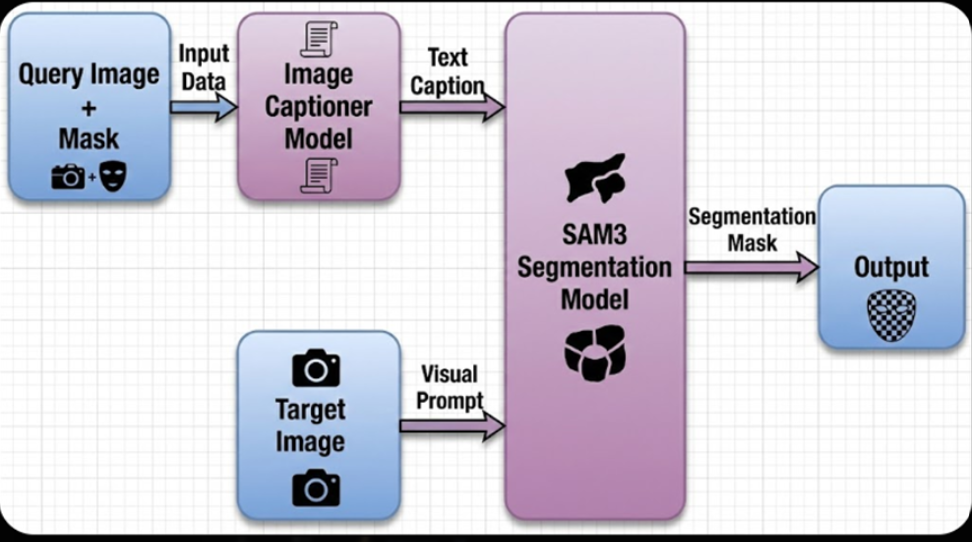
\includegraphics[width=1\linewidth]{SAM3.png}%
}{%
    \framebox[\linewidth]{\rule{0pt}{200pt}\textbf{Missing Image: SAM3.png}}%
}
\caption{PerSAM SAM3 Pipeline.}
\label{fig:SAM3}
\end{figure}

\begin{table}[htbp]
\centering
\caption{Aggregated Comparison: SAM3 vs PerSAM Frameworks}
\label{tab:sam3_comparison}
\begin{tabular}{l c | c c | c c}
\toprule
\textbf{Metric} & \textbf{SAM3 (Text)} & \textbf{Rep. PerSAM} & \textbf{$\Delta$ (vs PerSAM)} & \textbf{Rep. PerSAM-F} & \textbf{$\Delta$ (vs PerSAM-F)} \\
\midrule
mIoU & 95.15\% & 89.32\% & +5.83\% & 95.18\% & $-0.03\%$ \\
\bottomrule
\end{tabular}
\end{table}

\textbf{Key Takeaways.} Against the reproduced PerSAM, SAM3 is higher in mIoU by +5.83\%, mainly because PerSAM collapses on a few objects (e.g., Can, Teapot, RC Car, Robot Toy, Candle). Against the reproduced PerSAM-F, SAM3 is essentially tied ($-0.03\%$ mIoU). The pipeline achieved performance comparable to PerSAM-F while relying only on text captions (no personalized image-based signals). This indicates that PerSeg is suboptimal for evaluating personalized segmentation, since strong results can be obtained without true personalization cues.

\small
\setlength{\tabcolsep}{4pt}
\begin{longtable}{l c c c c c}
\caption{Per-Object mIoU Comparison: SAM3 vs PerSAM Frameworks} \label{tab:sam3_per_object} \\
\toprule
\textbf{Object} & \textbf{SAM3} & \textbf{Rep. PerSAM} & \textbf{$\Delta$ vs PerSAM} & \textbf{Rep. PerSAM-F} & \textbf{$\Delta$ vs PerSAM-F} \\ \midrule
\endfirsthead
\caption[]{Per-Object mIoU Comparison: SAM3 vs PerSAM Frameworks (Continued)} \\
\toprule
\textbf{Object} & \textbf{SAM3} & \textbf{Rep. PerSAM} & \textbf{$\Delta$ vs PerSAM} & \textbf{Rep. PerSAM-F} & \textbf{$\Delta$ vs PerSAM-F} \\ \midrule
\endhead
\midrule \multicolumn{6}{r}{\textit{Continued on next page}} \\
\endfoot
\bottomrule
\endlastfoot
Backpack & 96.48\% & 96.17\% & +0.31\% & 96.66\% & $-0.18\%$ \\
Backpack Dog & 96.39\% & 95.85\% & +0.54\% & 95.76\% & +0.63\% \\
Barn & 96.33\% & 96.19\% & +0.14\% & 95.17\% & +1.16\% \\
Bear Plushie & 95.41\% & 89.28\% & +6.13\% & 95.32\% & +0.09\% \\
Berry Bowl & 93.97\% & 91.81\% & +2.16\% & 91.27\% & +2.70\% \\
Can & 97.40\% & 38.91\% & +58.49\% & 97.49\% & $-0.09\%$ \\
Candle & 95.42\% & 74.16\% & +21.26\% & 96.76\% & $-1.34\%$ \\
Cat & 94.59\% & 95.54\% & $-0.95\%$ & 95.51\% & $-0.92\%$ \\
Cat 2 & 93.06\% & 94.72\% & $-1.66\%$ & 94.05\% & $-0.99\%$ \\
Cat Statue & 89.07\% & 95.42\% & $-6.35\%$ & 95.46\% & $-6.39\%$ \\
Chair & 92.49\% & 92.23\% & +0.26\% & 92.14\% & +0.35\% \\
Clock & 95.62\% & 90.70\% & +4.92\% & 94.79\% & +0.83\% \\
Colorful Sneaker & 93.96\% & 94.48\% & $-0.52\%$ & 95.13\% & $-1.17\%$ \\
Colorful Teapot & 96.45\% & 96.27\% & +0.18\% & 84.47\% & +11.98\% \\
Dog & 96.20\% & 96.79\% & $-0.59\%$ & 96.81\% & $-0.61\%$ \\
Dog 2 & 94.62\% & 95.66\% & $-1.04\%$ & 95.79\% & $-1.17\%$ \\
Dog 3 & 92.99\% & 88.85\% & +4.14\% & 88.67\% & +4.32\% \\
Dog 4 & 94.61\% & 95.22\% & $-0.61\%$ & 95.18\% & $-0.57\%$ \\
Dog 5 & 96.29\% & 97.10\% & $-0.81\%$ & 97.22\% & $-0.93\%$ \\
Dog 6 & 93.69\% & 94.66\% & $-0.97\%$ & 94.85\% & $-1.16\%$ \\
Dog 7 & 92.41\% & 93.69\% & $-1.28\%$ & 93.77\% & $-1.36\%$ \\
Dog 8 & 95.10\% & 95.34\% & $-0.24\%$ & 95.61\% & $-0.51\%$ \\
Duck Toy & 97.47\% & 97.31\% & +0.16\% & 97.31\% & +0.16\% \\
Elephant & 95.83\% & 96.05\% & $-0.22\%$ & 96.07\% & $-0.24\%$ \\
Fancy Boot & 95.06\% & 95.87\% & $-0.81\%$ & 95.96\% & $-0.90\%$ \\
Grey Sloth Plushie & 95.67\% & 96.37\% & $-0.70\%$ & 96.64\% & $-0.97\%$ \\
Monster Toy & 93.73\% & 93.75\% & $-0.02\%$ & 94.21\% & $-0.48\%$ \\
Poop Emoji & 94.29\% & 96.01\% & $-1.72\%$ & 96.43\% & $-2.14\%$ \\
RC Car & 96.25\% & 39.30\% & +56.95\% & 96.12\% & +0.13\% \\
Red Cartoon & 96.48\% & 96.96\% & $-0.48\%$ & 97.11\% & $-0.63\%$ \\
Robot Toy & 96.30\% & 60.55\% & +35.75\% & 96.66\% & $-0.36\%$ \\
Round Bird & 96.52\% & 96.79\% & $-0.27\%$ & 96.85\% & $-0.33\%$ \\
Shiny Sneaker & 96.56\% & 97.00\% & $-0.44\%$ & 96.87\% & $-0.31\%$ \\
Table & 94.66\% & 94.68\% & $-0.02\%$ & 94.66\% & +0.00\% \\
Teapot & 97.15\% & 40.02\% & +57.13\% & 96.93\% & +0.22\% \\
Teddy Bear & 96.03\% & 94.63\% & +1.40\% & 94.61\% & +1.42\% \\
Thin Bird & 93.36\% & 93.72\% & $-0.36\%$ & 93.96\% & $-0.60\%$ \\
Tortoise Plushy & 96.99\% & 93.06\% & +3.93\% & 97.09\% & $-0.10\%$ \\
Wolf Plushie & 94.34\% & 94.34\% & $-0.50\%$ & 94.32\% & $-0.48\%$ \\
Wooden Pot & 97.38\% & 97.42\% & $-0.04\%$ & 97.43\% & $-0.05\%$ \\
\end{longtable}
\normalsize

{\footnotesize
\setlength{\tabcolsep}{4pt}
\begin{longtable}{l p{10cm}}
\caption{Caption Static Mapping used for SAM3 Evaluation on PerSeg} \label{tab:sam3_captions} \\
\toprule
\textbf{Object ID} & \textbf{Caption Provided to SAM3} \\ \midrule
\endfirsthead
\caption[]{Caption Static Mapping used for SAM3 Evaluation (Continued)} \\
\toprule
\textbf{Object ID} & \textbf{Caption Provided to SAM3} \\ \midrule
\endhead
\midrule \multicolumn{2}{r}{\textit{Continued on next page}} \\
\endfoot
\bottomrule
\endlastfoot
backpack & backpack \\
backpack\_dog & gray backpack \\
barn & barn \\
bear\_plushie & A brown teddy bear with a blue hat on its head. \\
berry\_bowl & berry bowl \\
can & silver beverage can \\
candle & a white candle with a wooden lid on a white background \\
cat & cat \\
cat2 & cat \\
cat\_statue & cat statue \\
chair & chair \\
clock & A copper alarm clock with a crown on the face. \\
colorful\_sneaker & colorful sneaker \\
colorful\_teapot & A colorful teapot with a flower design on it. \\
dog & A dog with its tongue out. \\
dog2 & A brown dog with long hair and a big smile on its face. \\
dog3 & dog \\
dog4 & dog \\
dog5 & dog \\
dog6 & dog \\
dog7 & dog \\
dog8 & dog \\
duck\_toy & duck toy \\
elephant & elephant \\
fancy\_boot & fancy fashion boot \\
grey\_sloth\_plushie & grey sloth plushie \\
monster\_toy & monster toy \\
poop\_emoji & A close up of a poop emoji with big eyes. \\
rc\_car & A toy race car with a man in a helmet driving a red and yellow car. \\
red\_cartoon & red cartoon \\
robot\_toy & robot toy \\
round\_bird & A round bird figurine with a brown beak. \\
shiny\_sneaker & shiny sneaker with white soles. \\
table & a round coffee table with a wooden top and metal frame \\
teapot & teapot \\
teddybear & teddy bear \\
thin\_bird & A thin white bird's figurine. \\
tortoise\_plushy & green tortoise plush toy \\
wolf\_plushie & A gray and white husky dog plushie with a red collar laying down. \\
wooden\_pot & A wooden vase pot with a carved design on it. \\
\end{longtable}
}

\newpage


% --- DAPSAM Section ---
\section{DAPSAM: Domain Adaptation for Medical Segmentation \cite{wei2024prompting}}

\subsection{Implementation Details of Enhancements}
Applying generic visual foundation models to the medical domain presents massive structural challenges. Initial reproductions of the Domain-Adaptive Prototype SAM (DAPSAM) exhibited degradations under severe domain shift. To improve adapter robustness and feature integration, a series of structural enhancements were successfully implemented:
\begin{itemize}
    \item \textbf{Residual Scaling:} The standard residual connection $x + x_s$ was replaced with a parameterized adaptation $x + \text{residual\_scale} \times x_s$. This allowed the model to dynamically balance its strong pre-trained natural-image priors with the learned medical-domain features.
    \item \textbf{Dropout Regularization:} A light dropout rate of 0.1 was introduced within the adapter layers. This mitigated the risk of the adapter modules overfitting to the limited and homogenous clinical datasets.
    \item \textbf{MLP Ratio Optimization:} The hidden layer expansion ratio within the adapter block was strictly bounded at 0.25; experimental ablation demonstrated that expanding to 0.35 degraded generalization.
    \item \textbf{Skip Connections:} Architectural skip connections were rigorously maintained to ensure gradient stability across the multi-layer perceptron blocks.
\end{itemize}

\subsection{Evaluation on Prostate MRI Dataset}
The enhanced architecture was first evaluated on the multi-center Prostate MRI dataset, tracking both the Dice Similarity Coefficient (DSC) (higher is better) and Average Surface Distance (ASD, lower is better). 

\begin{table}[htbp]
\centering
\caption{Prostate Dataset: Original, Reproduced, and Enhanced DAPSAM Performance}
\label{tab:dapsam_prostate}
\resizebox{\linewidth}{!}{
\begin{tabular}{l c c c c c c c c c}
\toprule
\textbf{Domain} & \textbf{Orig. Dice} & \textbf{Repr. Dice} & \textbf{$\Delta$(Repr-Orig)} & \textbf{Repr. ASD} & \textbf{Enh. Dice} & \textbf{$\Delta$(Enh-Repr)} & \textbf{$\Delta$(Enh-Orig)} & \textbf{Enh. ASD} & \textbf{$\Delta$ASD (Enh-Repr)} \\
\midrule
A (RUNMC) & 86.34 & 85.48 & $-0.86$ & 2.60 & 86.71 & +1.23 & +0.37 & 2.08 & $-0.52$ \\
B (BMC)   & 81.05 & 80.62 & $-0.43$ & 7.53 & 80.40 & $-0.22$ & $-0.65$ & 7.07 & $-0.46$ \\
C (I2CVB) & 70.81 & 64.99 & $-5.82$ & 6.12 & 68.58 & +3.59 & $-2.23$ & 6.34 & +0.22 \\
D (UCL)   & 85.28 & 84.53 & $-0.75$ & 2.46 & 84.49 & $-0.04$ & $-0.79$ & 2.42 & $-0.04$ \\
E (BIDMC) & 82.91 & 83.13 & +0.22 & 4.30 & 83.53 & +0.40 & +0.62 & 3.80 & $-0.50$ \\
F (HK)    & 81.48 & 79.57 & $-1.91$ & 6.51 & 81.14 & +1.57 & $-0.34$ & 5.67 & $-0.84$ \\
\midrule
\textbf{Average} & \textbf{81.31} & \textbf{79.72} & \textbf{$-1.59$} & \textbf{4.59} & \textbf{80.81} & \textbf{+1.09} & \textbf{$-0.50$} & \textbf{4.23} & \textbf{$-0.36$} \\
\bottomrule
\end{tabular}}
\end{table}

While the initial reproduction exhibited an average Dice degradation of 1.59\% (with a severe 5.82\% drop on Domain C likely due to severe distribution shift), the enhanced pipeline successfully recovered +1.09\% average Dice accuracy. Crucially, the enhanced model achieved a 0.36 reduction in ASD, indicating significantly cleaner boundary delineation.

\subsection{Evaluation on RIGA+ Dataset}
Further evaluation was conducted on the RIGA+ Fundus benchmarks, evaluating the segmentation quality of the Optic Disc, measured via the Disc Overlap Dice (DOD), and the Optic Cup, measured via the Cup Overlap Dice (DOC), across two distinct sources (BinRushed and Magrabia). 

\begin{table}[htbp]
\centering
\caption{RIGA+ Dataset Performance (Source: BinRushed) - Dice Score \%}
\label{tab:dapsam_riga_binrushed}
\resizebox{\linewidth}{!}{
\begin{tabular}{l c c c c c c c c}
\toprule
\textbf{Target} & \textbf{Orig. ($\pm$ Std)} & \textbf{Repr.} & \textbf{$\Delta$(Repr-Orig)} & \textbf{Repr. Within Std?} & \textbf{Enh.} & \textbf{$\Delta$(Enh-Repr)} & \textbf{$\Delta$(Enh-Orig)} & \textbf{Enh. Within Std?} \\
\midrule
BASE1-DOD & 96.34 $\pm$ 0.17 & 96.37 & +0.03 & Yes & 96.29 & $-0.08$ & $-0.05$ & Yes \\
BASE1-DOC & 88.24 $\pm$ 0.16 & 87.21 & $-1.03$ & No & 87.50 & +0.29 & $-0.74$ & No \\
BASE2-DOD & 96.10 $\pm$ 0.10 & 95.76 & $-0.34$ & No & 95.79 & +0.03 & $-0.31$ & No \\
BASE2-DOC & 86.31 $\pm$ 0.13 & 83.87 & $-2.44$ & No & 85.67 & +1.80 & $-0.64$ & No \\
BASE3-DOD & 96.34 $\pm$ 0.14 & 96.21 & $-0.13$ & Yes & 96.17 & $-0.04$ & $-0.17$ & No \\
BASE3-DOC & 88.77 $\pm$ 0.21 & 86.25 & $-2.52$ & No & 86.94 & +0.69 & $-1.83$ & No \\
\midrule
\textbf{DOD Avg} & 96.26 & 96.11 & $-0.15$ & -- & 96.08 & $-0.03$ & $-0.18$ & -- \\
\textbf{DOC Avg} & 87.87 & 85.78 & $-2.09$ & -- & 86.70 & +0.92 & $-1.17$ & -- \\
\bottomrule
\end{tabular}}
\end{table}

\begin{table}[htbp]
\centering
\caption{RIGA+ Dataset Performance (Source: Magrabia) - Dice Score \%}
\label{tab:dapsam_riga_magrabia}
\resizebox{\linewidth}{!}{
\begin{tabular}{l c c c c c c c c}
\toprule
\textbf{Target} & \textbf{Orig. ($\pm$ Std)} & \textbf{Repr.} & \textbf{$\Delta$(Repr-Orig)} & \textbf{Repr. Within Std?} & \textbf{Enh.} & \textbf{$\Delta$(Enh-Repr)} & \textbf{$\Delta$(Enh-Orig)} & \textbf{Enh. Within Std?} \\
\midrule
BASE1-DOD & 96.22 $\pm$ 0.18 & 95.60 & $-0.62$ & No & 95.60 & 0.00 & $-0.62$ & No \\
BASE1-DOC & 86.74 $\pm$ 0.36 & 87.69 & +0.95 & Yes & 87.99 & +0.30 & +1.25 & No \\
BASE2-DOD & 96.32 $\pm$ 0.16 & 95.49 & $-0.83$ & No & 95.44 & $-0.05$ & $-0.88$ & No \\
BASE2-DOC & 89.59 $\pm$ 0.24 & 87.71 & $-1.88$ & No & 88.19 & +0.48 & $-1.40$ & No \\
BASE3-DOD & 96.35 $\pm$ 0.20 & 95.59 & $-0.76$ & No & 95.59 & 0.00 & $-0.76$ & No \\
BASE3-DOC & 88.12 $\pm$ 0.22 & 88.76 & +0.64 & Yes & 88.78 & +0.02 & +0.66 & Yes \\
\midrule
\textbf{DOD Avg} & 96.30 & 95.56 & $-0.74$ & -- & 95.54 & $-0.02$ & $-0.76$ & -- \\
\textbf{DOC Avg} & 88.15 & 88.05 & $-0.10$ & -- & 88.32 & +0.27 & +0.17 & -- \\
\bottomrule
\end{tabular}}
\end{table}

\subsection{General Results Discussion}
The multi-domain enhancement trial yielded highly consistent trends regarding structural ambiguity. The Optic Cup (DOC) naturally lacks distinct structural boundaries compared to the Optic Disc (DOD), making it significantly more susceptible to domain shift during feature extraction.
\begin{itemize}
    \item \textbf{Reproduction vs. Original:} The pure reproduction exhibited acceptable fidelity on the easier DOD metrics (Dice drops of only 0.15\% to 0.74\%), but struggled with the harder, low-contrast DOC boundaries, leading to larger deviations (up to 2.09\% degradation) and matching the issues seen in the Prostate MRI (1.59\% degradation).
    \item \textbf{Enhancement vs. Reproduction:} The proposed architectural enhancements effectively arrested these degradations. On Prostate MRI, enhancements recovered 1.09\% in Dice and improved ASD by 0.36. On RIGA+, the most substantial gains were precisely where the reproduction struggled the most—the DOC targets (gaining +0.92\% on BinRushed and +0.27\% on Magrabia). The residual scaling efficiently stabilized the feature extraction in these ambiguous regions.
    \item \textbf{Conclusion:} The implemented enhancements consistently improve adapter generalization and robustness over the standard reproduced versions, contributing to better feature integration and significantly improved boundary alignment (ASD). While the enhanced models do not fully reconstruct the absolute highest metrics reported in the original manuscript for DOD targets, they stabilize and secure the more challenging DOC and multi-center MRI domains against severe distribution shifts.
\end{itemize}


% ==========================================
% CHAPTER 7: PROPOSED PHD RESEARCH DIRECTIONS
% ==========================================
\chapter{Proposed PhD Research Directions}

\section{Improving Prompt Robustness and Stability}
Prompt-based conditioning is a central mechanism in adapting foundation models for few-shot segmentation. However, existing approaches are highly sensitive to variations in support examples and spatial ambiguity near object boundaries. 

This research direction focuses on improving the robustness and stability of prompt representations through:
\begin{itemize}
    \item Developing simple uncertainty-aware strategies such as prompt averaging, confidence-based weighting, and multi-prompt aggregation.
    \item Designing robust prompt selection mechanisms that reduce sensitivity to noisy or imperfect support masks.
    \item Systematically evaluating the impact of prompt variability on segmentation consistency across datasets and shot settings.
\end{itemize}

\section{Efficient Cross-Image Feature Alignment}
Accurate correspondence between support and query images remains a fundamental challenge in few-shot segmentation. While dense feature matching improves accuracy, it introduces significant computational overhead.

This direction aims to:
\begin{itemize}
    \item Investigate lightweight feature alignment mechanisms that improve correspondence without excessive cost.
    \item Combine prompt-based conditioning with selective feature matching to leverage strengths of both paradigms.
    \item Introduce filtering or attention strategies to suppress distractors in cluttered multi-instance scenes.
\end{itemize}

\section{Robustness to Complex Scenes and Domain Shift}
Current methods often degrade in scenarios involving occlusion, scale variation, or domain shifts (e.g., moving from natural images to structured datasets).

This direction focuses on:
\begin{itemize}
    \item Conducting systematic failure analysis in multi-instance and highly cluttered environments.
    \item Introducing simple structural constraints such as spatial consistency enforcement or region filtering.
    \item Evaluating robustness across datasets of increasing complexity (COCO-20$^i$, LVIS, and part-level benchmarks).
\end{itemize}

\section{Lightweight Adaptation Strategies}
Rather than introducing heavy architectural modifications, this work emphasizes efficient adaptation mechanisms compatible with frozen foundation models.

This includes:
\begin{itemize}
    \item Exploring parameter-efficient modules such as lightweight adapters or refinement layers.
    \item Preserving the frozen SAM backbone to maintain computational efficiency.
    \item Studying the trade-off between performance improvement and additional computational cost.
\end{itemize}

\section{Practical Deployment Considerations}
To ensure applicability in real-world scenarios, deployment constraints must be considered.

This direction aims to:
\begin{itemize}
    \item Analyze inference latency and memory usage across different methods.
    \item Optimize selected approaches for reduced computational overhead.
    \item Evaluate feasibility for deployment on resource-constrained environments.
\end{itemize}


% ==========================================
% CHAPTER 8: EXPECTED CONTRIBUTIONS AND RESEARCH PLAN
% ==========================================
\chapter{Expected Contributions and Research Plan}

\section{Expected Contributions}
\begin{itemize}
    \item A comprehensive and reproducible evaluation of SAM-based few-shot segmentation methods under unified experimental settings.
    \item A systematic analysis of key failure modes, including prompt sensitivity, boundary ambiguity, and distractor confusion.
    \item A lightweight conditioning framework that improves robustness while preserving computational efficiency.
    \item Empirical insights into the trade-offs between accuracy, robustness, and computational cost.
    \item Standardized evaluation protocols and benchmarks to support future research in this domain.
\end{itemize}

\section{Research Plan and Phases}
\begin{enumerate}
    \item \textbf{Phase 1: Baseline Reproduction and Benchmarking}
    \begin{itemize}
        \item Reproduce core baselines (VRP-SAM, ProSAM, Matcher, DC-SAM, FCP-SAM, PerSAM).
        \item Standardize evaluation protocols across PASCAL-5$^i$, COCO-20$^i$, and part-level datasets.
        \item Establish unified metrics (mIoU, Dice, FPS, memory footprint).
    \end{itemize}
    
    \item \textbf{Phase 2: Failure Mode Analysis}
    \begin{itemize}
        \item Analyze segmentation failures in boundary regions and cluttered scenes.
        \item Evaluate sensitivity to prompt quality and number of support examples.
        \item Identify computational bottlenecks across methods.
    \end{itemize}
    
    \item \textbf{Phase 3: Method Development}
    \begin{itemize}
        \item Design a lightweight conditioning framework combining prompt-based and feature-based strategies.
        \item Introduce mechanisms for improving robustness (e.g., prompt refinement or feature filtering).
        \item Ensure compatibility with frozen foundation models.
    \end{itemize}
    
    \item \textbf{Phase 4: Extended Evaluation}
    \begin{itemize}
        \item Conduct ablation studies to evaluate individual components.
        \item Test generalization on large-vocabulary datasets (FSS-1000, LVIS-92$^i$).
        \item Evaluate performance under domain shift and complex scene conditions.
    \end{itemize}
    
    \item \textbf{Phase 5: Efficiency Optimization}
    \begin{itemize}
        \item Optimize inference pipeline for reduced latency and memory usage.
        \item Compare performance-efficiency trade-offs across models.
        \item Explore deployment feasibility on constrained hardware.
    \end{itemize}
    
    \item \textbf{Phase 6: Thesis Consolidation and Publication}
    \begin{itemize}
        \item Integrate results into a unified framework.
        \item Prepare publications targeting top-tier venues (e.g., CVPR, ICCV, TPAMI).
    \end{itemize}
\end{enumerate}


% ==========================================
% CHAPTER 9: CONCLUSION
% ==========================================
\chapter{Conclusion}

This report examined reference-guided few-shot segmentation with foundation models, with a focus on adapting SAM to class-agnostic segmentation tasks. The analysis highlighted that, despite strong geometric representations, current approaches still face challenges in achieving reliable semantic alignment between support and query images.  

The proposed taxonomy provided a structured view of existing methods, clarifying the differences between prompt-based, matching-based, and more advanced reasoning approaches. The comparison across datasets showed clear trade-offs between efficiency and robustness, and emphasized the impact of scene complexity, distractors, and domain shift on model performance.  

The report also presented the work completed so far in the PhD, including reproductions of representative methods and corresponding experimental results. These efforts offered practical insights into the implementation and behavior of different approaches, and helped validate several observations regarding prompt sensitivity, structural limitations, and performance variations across scenarios.  

Building on these findings, the report outlined a set of research directions for the next stage of the PhD. These include improving conditioning mechanisms, enhancing robustness to domain variability, and exploring more efficient adaptation strategies.  

Overall, the report consolidates current understanding, supports it with experimental observations, and establishes a clear basis for the subsequent research phase.

\newpage


% ==========================================
% REFERENCES
% ==========================================
\begin{thebibliography}{10}

\bibitem{kirillov2023segment}
Kirillov, A., Mintun, E., Ravi, N., Mao, H., Rolland, C., Gustafson, L., ... \& Girshick, R. (2023). Segment anything. In \textit{Proceedings of the IEEE/CVF International Conference on Computer Vision} (pp. 4015-4026).

\bibitem{he2016deep}
He, K., Zhang, X., Ren, S., \& Sun, J. (2016). Deep residual learning for image recognition. In \textit{Proceedings of the IEEE conference on computer vision and pattern recognition} (pp. 770-778).

\bibitem{oquab2023dinov2}
Oquab, M., Darcet, T., Moutakanni, T., Vo, H., Szafraniec, M., Khalidov, V., ... \& Bojanowski, P. (2023). Dinov2: Learning robust visual features without supervision. \textit{arXiv preprint arXiv:2304.07193}.

\bibitem{dosovitskiy2020image}
Dosovitskiy, A., Beyer, L., Kolesnikov, A., Weissenborn, D., Zhai, X., Unterthiner, T., ... \& Houlsby, N. (2020). An image is worth 16x16 words: Transformers for image recognition at scale. \textit{International Conference on Learning Representations}.

\bibitem{shaban2017one}
Shaban, A., Bansal, S., Liu, Z., Essa, I., \& Boots, B. (2017). One-shot learning for semantic segmentation. In \textit{Proceedings of the British Machine Vision Conference (BMVC)}.

\bibitem{nguyen2019feature}
Nguyen, K., \& Todorovic, S. (2019). Feature weighting and boosting for few-shot segmentation. In \textit{Proceedings of the IEEE/CVF International Conference on Computer Vision} (pp. 622-631).

\bibitem{everingham2010pascal}
Everingham, M., Van Gool, L., Williams, C. K., Winn, J., \& Zisserman, A. (2010). The pascal visual object classes (voc) challenge. \textit{International journal of computer vision}, 88(2), 303-338.

\bibitem{lin2014microsoft}
Lin, T. Y., Maire, M., Belongie, S., Hays, J., Perona, P., Ramanan, D., ... \& Zitnick, C. L. (2014). Microsoft coco: Common objects in context. In \textit{European conference on computer vision} (pp. 740-755). Springer, Cham.

\bibitem{li2020fss}
Li, X., Wei, T., Chen, Y. P., Tai, Y.-W., \& Tang, C.-K. (2020). Fss-1000: A 1000-class dataset for few-shot segmentation. In \textit{Proceedings of the IEEE/CVF conference on computer vision and pattern recognition} (pp. 2869-2878).

\bibitem{gupta2019lvis}
Gupta, A., Dollar, P., \& Girshick, R. (2019). Lvis: A dataset for large vocabulary instance segmentation. In \textit{Proceedings of the IEEE/CVF conference on computer vision and pattern recognition} (pp. 5356-5364).

\bibitem{chen2014detect}
Chen, X., Mottaghi, R., Liu, X., Fidler, S., Urtasun, R., \& Yuille, A. (2014). Detect what you can: Detecting and representing objects using holistic models and body parts. In \textit{Proceedings of the IEEE conference on computer vision and pattern recognition} (pp. 1971-1978).

\bibitem{ramanathan2023paco}
Ramanathan, V., Kalia, A., Petrovic, V., Wen, Y., Zheng, B., Guo, B., ... \& Marquez, A. (2023). Paco: Parts and attributes of common objects. \textit{arXiv preprint arXiv:2301.01795}.

\bibitem{wang2019panet}
Wang, K., Liew, J. H., Zou, Y., Zhou, D., \& Feng, J. (2019). PANet: Few-shot image semantic segmentation with prototype alignment. In \textit{Proceedings of the IEEE/CVF International Conference on Computer Vision} (pp. 9197-9206).

\bibitem{tian2020pfenet}
Tian, Z., Zhao, H., Shu, M., Yang, Z., Li, R., \& Jia, J. (2020). Prior guided feature enrichment network for few-shot segmentation. \textit{IEEE Transactions on Pattern Analysis and Machine Intelligence}, 44(2), 1050-1065.

\bibitem{sun2024vrp}
Sun, Y., Chen, J., Zhang, S., Zhang, X., Chen, Q., Zhang, G., \& Li, Z. (2024).
VRP-SAM: SAM with visual reference prompt.
In \textit{Proceedings of the IEEE/CVF Conference on Computer Vision and Pattern Recognition (CVPR)} (pp. 23565--23574).

\bibitem{wang2025prosam}
Wang, X., Sebastian, C., He, W., \& Ren, L. (2025).
ProSAM: Enhancing the robustness of SAM-based visual reference segmentation with probabilistic prompts.
In \textit{Proceedings of the IEEE/CVF International Conference on Computer Vision (ICCV)} (pp. 20487--20496).

\bibitem{liu2023matcher}
Liu, Y., Zhu, M., Li, H., Chen, H., Wang, X., \& Shen, C. (2023).
Matcher: Segment anything with one shot using all-purpose feature matching.
\textit{arXiv preprint arXiv:2305.13310}.

\bibitem{qi2025dcsam}
Qi, M., Zhu, P., Li, X., Bi, X., Qi, L., Ma, H., \& Yang, M. H. (2025).
DC-SAM: In-context segment anything in images and videos via dual consistency.
\textit{IEEE Transactions on Pattern Analysis and Machine Intelligence}.

\bibitem{zhang2024bridge}
Zhang, A., Gao, G., Jiao, J., Liu, C., \& Wei, Y. (2024).
Bridge the points: Graph-based few-shot segment anything semantically.
In \textit{Advances in Neural Information Processing Systems (NeurIPS)}, 37, 33232--33261.

\bibitem{park2025fcpsam}
Park, S., Lee, S., Seong, H. S., Yoo, J., \& Heo, J. P. (2025).
Foreground-covering prototype generation and matching for SAM-aided few-shot segmentation.
In \textit{Proceedings of the AAAI Conference on Artificial Intelligence}, 39(6), 6425--6433.

\bibitem{zhang2024persam}
Zhang, R., Jiang, Z., Guo, Z., Yan, S., Pan, J., Dong, H., ... \& Gao, P. (2024). 
Personalize segment anything model with one shot.
In \textit{International Conference on Learning Representations (ICLR)}.

\bibitem{wei2024prompting}
Wei, Z., Dong, W., Zhou, P., Gu, Y., Zhao, Z., \& Xu, Y. (2024). 
Prompting segment anything model with domain-adaptive prototype for generalizable medical image segmentation. 
In \textit{International conference on medical image computing and computer-assisted intervention} (pp. 533--543). Springer.

\bibitem{pont2017the}
Pont-Tuset, J., Perazzi, F., Marques, S., Garcia, J., \& Van Gool, L. (2017). 
The 2017 davis challenge on video object segmentation. 
\textit{arXiv preprint arXiv:1704.00675}.

\bibitem{ravi2024sam2}
Ravi, N., Gabeur, V., Hu, Y. T., Hu, R., Ryali, C., Ma, T., \& Feichtenhofer, C. (2024).
SAM 2: Segment anything in images and videos.
\textit{arXiv preprint arXiv:2408.00714}.

\bibitem{carion2025sam3}
Carion, N., Gustafson, L., Hu, Y. T., Debnath, S., Hu, R., Suris, D., \& Feichtenhofer, C. (2025).
SAM 3: Segment anything with concepts.
\textit{arXiv preprint arXiv:2511.16719}.

\bibitem{wortsman2022modelsoups}
Wortsman, M., Ilharco, G., Gadre, S. Y., Roelofs, R., Gontijo-Lopes, R., Morcos, A. S., \& Schmidt, L. (2022).
Model soups: Averaging weights of multiple fine-tuned models improves accuracy without increasing inference time.
In \textit{Proceedings of the 39th International Conference on Machine Learning (ICML)} (pp. 23965--23998). PMLR.

\bibitem{wasfy2023enhancing}
Wasfy, O., Basiony, S., \& Torki, M. (2023).
Enhancing LiDAR Semantic Segmentation Using Model Soups.
In \textit{2023 20th ACS/IEEE International Conference on Computer Systems and Applications (AICCSA)} (pp. 1--7). IEEE.

\end{thebibliography}

\end{document}
